% Options for packages loaded elsewhere
% Options for packages loaded elsewhere
\PassOptionsToPackage{unicode}{hyperref}
\PassOptionsToPackage{hyphens}{url}
\PassOptionsToPackage{dvipsnames,svgnames,x11names}{xcolor}
%
\documentclass[
  french,
  letterpaper,
  DIV=11,
  numbers=noendperiod]{scrreprt}
\usepackage{xcolor}
\usepackage{amsmath,amssymb}
\setcounter{secnumdepth}{5}
\usepackage{iftex}
\ifPDFTeX
  \usepackage[T1]{fontenc}
  \usepackage[utf8]{inputenc}
  \usepackage{textcomp} % provide euro and other symbols
\else % if luatex or xetex
  \usepackage{unicode-math} % this also loads fontspec
  \defaultfontfeatures{Scale=MatchLowercase}
  \defaultfontfeatures[\rmfamily]{Ligatures=TeX,Scale=1}
\fi
\usepackage{lmodern}
\ifPDFTeX\else
  % xetex/luatex font selection
\fi
% Use upquote if available, for straight quotes in verbatim environments
\IfFileExists{upquote.sty}{\usepackage{upquote}}{}
\IfFileExists{microtype.sty}{% use microtype if available
  \usepackage[]{microtype}
  \UseMicrotypeSet[protrusion]{basicmath} % disable protrusion for tt fonts
}{}
\makeatletter
\@ifundefined{KOMAClassName}{% if non-KOMA class
  \IfFileExists{parskip.sty}{%
    \usepackage{parskip}
  }{% else
    \setlength{\parindent}{0pt}
    \setlength{\parskip}{6pt plus 2pt minus 1pt}}
}{% if KOMA class
  \KOMAoptions{parskip=half}}
\makeatother
% Make \paragraph and \subparagraph free-standing
\makeatletter
\ifx\paragraph\undefined\else
  \let\oldparagraph\paragraph
  \renewcommand{\paragraph}{
    \@ifstar
      \xxxParagraphStar
      \xxxParagraphNoStar
  }
  \newcommand{\xxxParagraphStar}[1]{\oldparagraph*{#1}\mbox{}}
  \newcommand{\xxxParagraphNoStar}[1]{\oldparagraph{#1}\mbox{}}
\fi
\ifx\subparagraph\undefined\else
  \let\oldsubparagraph\subparagraph
  \renewcommand{\subparagraph}{
    \@ifstar
      \xxxSubParagraphStar
      \xxxSubParagraphNoStar
  }
  \newcommand{\xxxSubParagraphStar}[1]{\oldsubparagraph*{#1}\mbox{}}
  \newcommand{\xxxSubParagraphNoStar}[1]{\oldsubparagraph{#1}\mbox{}}
\fi
\makeatother

\usepackage{color}
\usepackage{fancyvrb}
\newcommand{\VerbBar}{|}
\newcommand{\VERB}{\Verb[commandchars=\\\{\}]}
\DefineVerbatimEnvironment{Highlighting}{Verbatim}{commandchars=\\\{\}}
% Add ',fontsize=\small' for more characters per line
\usepackage{framed}
\definecolor{shadecolor}{RGB}{241,243,245}
\newenvironment{Shaded}{\begin{snugshade}}{\end{snugshade}}
\newcommand{\AlertTok}[1]{\textcolor[rgb]{0.68,0.00,0.00}{#1}}
\newcommand{\AnnotationTok}[1]{\textcolor[rgb]{0.37,0.37,0.37}{#1}}
\newcommand{\AttributeTok}[1]{\textcolor[rgb]{0.40,0.45,0.13}{#1}}
\newcommand{\BaseNTok}[1]{\textcolor[rgb]{0.68,0.00,0.00}{#1}}
\newcommand{\BuiltInTok}[1]{\textcolor[rgb]{0.00,0.23,0.31}{#1}}
\newcommand{\CharTok}[1]{\textcolor[rgb]{0.13,0.47,0.30}{#1}}
\newcommand{\CommentTok}[1]{\textcolor[rgb]{0.37,0.37,0.37}{#1}}
\newcommand{\CommentVarTok}[1]{\textcolor[rgb]{0.37,0.37,0.37}{\textit{#1}}}
\newcommand{\ConstantTok}[1]{\textcolor[rgb]{0.56,0.35,0.01}{#1}}
\newcommand{\ControlFlowTok}[1]{\textcolor[rgb]{0.00,0.23,0.31}{\textbf{#1}}}
\newcommand{\DataTypeTok}[1]{\textcolor[rgb]{0.68,0.00,0.00}{#1}}
\newcommand{\DecValTok}[1]{\textcolor[rgb]{0.68,0.00,0.00}{#1}}
\newcommand{\DocumentationTok}[1]{\textcolor[rgb]{0.37,0.37,0.37}{\textit{#1}}}
\newcommand{\ErrorTok}[1]{\textcolor[rgb]{0.68,0.00,0.00}{#1}}
\newcommand{\ExtensionTok}[1]{\textcolor[rgb]{0.00,0.23,0.31}{#1}}
\newcommand{\FloatTok}[1]{\textcolor[rgb]{0.68,0.00,0.00}{#1}}
\newcommand{\FunctionTok}[1]{\textcolor[rgb]{0.28,0.35,0.67}{#1}}
\newcommand{\ImportTok}[1]{\textcolor[rgb]{0.00,0.46,0.62}{#1}}
\newcommand{\InformationTok}[1]{\textcolor[rgb]{0.37,0.37,0.37}{#1}}
\newcommand{\KeywordTok}[1]{\textcolor[rgb]{0.00,0.23,0.31}{\textbf{#1}}}
\newcommand{\NormalTok}[1]{\textcolor[rgb]{0.00,0.23,0.31}{#1}}
\newcommand{\OperatorTok}[1]{\textcolor[rgb]{0.37,0.37,0.37}{#1}}
\newcommand{\OtherTok}[1]{\textcolor[rgb]{0.00,0.23,0.31}{#1}}
\newcommand{\PreprocessorTok}[1]{\textcolor[rgb]{0.68,0.00,0.00}{#1}}
\newcommand{\RegionMarkerTok}[1]{\textcolor[rgb]{0.00,0.23,0.31}{#1}}
\newcommand{\SpecialCharTok}[1]{\textcolor[rgb]{0.37,0.37,0.37}{#1}}
\newcommand{\SpecialStringTok}[1]{\textcolor[rgb]{0.13,0.47,0.30}{#1}}
\newcommand{\StringTok}[1]{\textcolor[rgb]{0.13,0.47,0.30}{#1}}
\newcommand{\VariableTok}[1]{\textcolor[rgb]{0.07,0.07,0.07}{#1}}
\newcommand{\VerbatimStringTok}[1]{\textcolor[rgb]{0.13,0.47,0.30}{#1}}
\newcommand{\WarningTok}[1]{\textcolor[rgb]{0.37,0.37,0.37}{\textit{#1}}}

\usepackage{longtable,booktabs,array}
\newcounter{none} % for unnumbered tables
\usepackage{calc} % for calculating minipage widths
% Correct order of tables after \paragraph or \subparagraph
\usepackage{etoolbox}
\makeatletter
\patchcmd\longtable{\par}{\if@noskipsec\mbox{}\fi\par}{}{}
\makeatother
% Allow footnotes in longtable head/foot
\IfFileExists{footnotehyper.sty}{\usepackage{footnotehyper}}{\usepackage{footnote}}
\makesavenoteenv{longtable}
\usepackage{graphicx}
\makeatletter
\newsavebox\pandoc@box
\newcommand*\pandocbounded[1]{% scales image to fit in text height/width
  \sbox\pandoc@box{#1}%
  \Gscale@div\@tempa{\textheight}{\dimexpr\ht\pandoc@box+\dp\pandoc@box\relax}%
  \Gscale@div\@tempb{\linewidth}{\wd\pandoc@box}%
  \ifdim\@tempb\p@<\@tempa\p@\let\@tempa\@tempb\fi% select the smaller of both
  \ifdim\@tempa\p@<\p@\scalebox{\@tempa}{\usebox\pandoc@box}%
  \else\usebox{\pandoc@box}%
  \fi%
}
% Set default figure placement to htbp
\def\fps@figure{htbp}
\makeatother


% definitions for citeproc citations
\NewDocumentCommand\citeproctext{}{}
\NewDocumentCommand\citeproc{mm}{%
  \begingroup\def\citeproctext{#2}\cite{#1}\endgroup}
\makeatletter
 % allow citations to break across lines
 \let\@cite@ofmt\@firstofone
 % avoid brackets around text for \cite:
 \def\@biblabel#1{}
 \def\@cite#1#2{{#1\if@tempswa , #2\fi}}
\makeatother
\newlength{\cslhangindent}
\setlength{\cslhangindent}{1.5em}
\newlength{\csllabelwidth}
\setlength{\csllabelwidth}{3em}
\newenvironment{CSLReferences}[2] % #1 hanging-indent, #2 entry-spacing
 {\begin{list}{}{%
  \setlength{\itemindent}{0pt}
  \setlength{\leftmargin}{0pt}
  \setlength{\parsep}{0pt}
  % turn on hanging indent if param 1 is 1
  \ifodd #1
   \setlength{\leftmargin}{\cslhangindent}
   \setlength{\itemindent}{-1\cslhangindent}
  \fi
  % set entry spacing
  \setlength{\itemsep}{#2\baselineskip}}}
 {\end{list}}
\usepackage{calc}
\newcommand{\CSLBlock}[1]{\hfill\break\parbox[t]{\linewidth}{\strut\ignorespaces#1\strut}}
\newcommand{\CSLLeftMargin}[1]{\parbox[t]{\csllabelwidth}{\strut#1\strut}}
\newcommand{\CSLRightInline}[1]{\parbox[t]{\linewidth - \csllabelwidth}{\strut#1\strut}}
\newcommand{\CSLIndent}[1]{\hspace{\cslhangindent}#1}

\ifLuaTeX
\usepackage[bidi=basic,shorthands=off]{babel}
\else
\usepackage[bidi=default,shorthands=off]{babel}
\fi
\ifLuaTeX
  \usepackage{selnolig} % disable illegal ligatures
\fi


\setlength{\emergencystretch}{3em} % prevent overfull lines

\providecommand{\tightlist}{%
  \setlength{\itemsep}{0pt}\setlength{\parskip}{0pt}}



 


\KOMAoption{captions}{tableheading}
\makeatletter
\@ifpackageloaded{bookmark}{}{\usepackage{bookmark}}
\makeatother
\makeatletter
\@ifpackageloaded{caption}{}{\usepackage{caption}}
\AtBeginDocument{%
\ifdefined\contentsname
  \renewcommand*\contentsname{Table des matières}
\else
  \newcommand\contentsname{Table des matières}
\fi
\ifdefined\listfigurename
  \renewcommand*\listfigurename{Liste des Figures}
\else
  \newcommand\listfigurename{Liste des Figures}
\fi
\ifdefined\listtablename
  \renewcommand*\listtablename{Liste des Tables}
\else
  \newcommand\listtablename{Liste des Tables}
\fi
\ifdefined\figurename
  \renewcommand*\figurename{Figure}
\else
  \newcommand\figurename{Figure}
\fi
\ifdefined\tablename
  \renewcommand*\tablename{Table}
\else
  \newcommand\tablename{Table}
\fi
}
\@ifpackageloaded{float}{}{\usepackage{float}}
\floatstyle{ruled}
\@ifundefined{c@chapter}{\newfloat{codelisting}{h}{lop}}{\newfloat{codelisting}{h}{lop}[chapter]}
\floatname{codelisting}{Listing}
\newcommand*\listoflistings{\listof{codelisting}{Liste des Listings}}
\makeatother
\makeatletter
\makeatother
\makeatletter
\@ifpackageloaded{caption}{}{\usepackage{caption}}
\@ifpackageloaded{subcaption}{}{\usepackage{subcaption}}
\makeatother
\usepackage{bookmark}
\IfFileExists{xurl.sty}{\usepackage{xurl}}{} % add URL line breaks if available
\urlstyle{same}
% fallback for those not using the hyperref driver hyperxmp:
\makeatletter
\@ifundefined{xmpquote}{\newcommand{\xmpquote}[1]{#1}}{}
\makeatother
\hypersetup{
  pdftitle={Régression II -- STT-4300},
  pdfauthor={Julien Miron},
  pdflang={fr},
  colorlinks=true,
  linkcolor={blue},
  filecolor={Maroon},
  citecolor={Blue},
  urlcolor={Blue},
  pdfcreator={LaTeX via pandoc}}


\title{\textbf{Régression II -- STT-4300}}
\author{Julien Miron}
\date{}
\begin{document}
\maketitle

\renewcommand*\contentsname{Table des matières}
{
\setcounter{tocdepth}{2}
\tableofcontents
}

\bookmarksetup{startatroot}

\chapter*{Préface}\label{pruxe9face}
\addcontentsline{toc}{chapter}{Préface}

\markboth{Préface}{Préface}

Ces notes de cours couvrent la régression linéaire, les modèles
linéaires généralisés (régression logistique, régression de Poisson),
les méthodes de validation et de sélection de modèles, la régularisation
(ridge, lasso), les méthodes de régression non-paramétrique (\(k\) plus
proches voisins, estimateur de noyau, splines) et les modèles additifs
généralisés (GAM).

Si vous constatez des coquilles ou des erreurs, merci de m'envoyer
\href{mailto:julien.miron@mat.ulaval.ca}{un courriel}.

\section*{Remerciements}\label{remerciements}
\addcontentsline{toc}{section}{Remerciements}

\markright{Remerciements}

Ces notes s'appuient en partie sur du matériel de cours développé
respectivement par Lajmi Lakhal Chaieb, Thierry Duchesne, Michel Carbon
et Khader Khadraoui de l'Université Laval et Eva Cantoni de l'Université
de Genève.

\section*{Utilisation de l'IA}\label{utilisation-de-lia}
\addcontentsline{toc}{section}{Utilisation de l'IA}

\markright{Utilisation de l'IA}

La rédaction de certains passages, ainsi que le développement de
certains exemples en R, ont bénéficié de l'assistance de Claude Sonnet
5, un modèle de langage développé par Anthropic.

\bookmarksetup{startatroot}

\chapter{Rappels de régression
linéaire}\label{rappels-de-ruxe9gression-linuxe9aire}

\section{Le modèle linéaire}\label{le-moduxe8le-linuxe9aire}

On dispose de données \(\{(Y_i, \boldsymbol{X}_i),\, i=1,\ldots,n\}\),
où \(Y_i\) est la variable réponse (continue) et
\(\boldsymbol{X}_i=(1,x_{i1},\ldots,x_{ip})^\top\) est un vecteur de
\(p\) variables explicatives\footnote{En régression, les variables
  explicatives sont souvent supposées connues (bien qu'on puisse les
  traiter comme étant des variables aléatoires). On utilise les
  majuscules pour les vecteurs ici, même s'ils sont composés de
  constantes et non de variables aléatoires.}. Le modèle de régression
linéaire multiple s'écrit :
\[Y_i = \beta_0 + \beta_1 x_{i1} + \cdots + \beta_p x_{ip} + \epsilon_i, \qquad i=1,\ldots,n,\]
où \(\beta_0,\beta_1,\ldots,\beta_p\) sont les coefficients de
régression et les erreurs \(\epsilon_i\) sont indépendantes et
identiquement distribuées selon \(\mathcal{N}(0,\sigma^2)\).

{Définition --- Matrice de design}

En écriture matricielle, on a
\(\boldsymbol{Y} = \boldsymbol{X\beta} + \epsilon\), où
\(\boldsymbol{Y}=(Y_1,\ldots,Y_n)^\top\),
\(\boldsymbol{\beta}=(\beta_0,\ldots,\beta_p)^\top\),
\(\boldsymbol{\epsilon}=(\epsilon_1,\ldots,\epsilon_n)^\top\) et
\(\boldsymbol{X}\) est la matrice de design (\emph{design
matrix})\footnote{Tout au long du document, certains termes seront
  traduits. Comme la plupart des références scientifiques en statistique
  sont en anglais, il peut être utile de connaître le terme en anglais
  afin de le reconnaître plus rapidement.} de dimension \(n\times(p+1)\)
dont la première colonne ne contient que des 1 pour inclure l'ordonnée à
l'origine : \[\boldsymbol{X} =
 \begin{pmatrix}  \boldsymbol{X}_1^\top \\  \vdots  \\   \boldsymbol{X}_n^\top\end{pmatrix}=\begin{pmatrix} 1 & x_{11} & \cdots & x_{1p} \\ \vdots & \vdots & & \vdots \\ 1 & x_{n1} & \cdots & x_{np}\end{pmatrix}.\]

Sous ces hypothèses, on a
\(\mu_i =E[Y_i|x_{i1},\ldots, x_{ip}] =  \beta_0 + \beta_1 x_{i1} + \cdots + \beta_p x_{ip}\)
et \(Var[Y_i] = \sigma^2\) (homoscédasticité).

\section{Estimation par moindres
carrés}\label{estimation-par-moindres-carruxe9s}

On estime \(\beta\) en minimisant la somme des carrés des écarts :
\[SS_E =\sum_{i=1}^n\epsilon_i^2= \sum_{i=1}^n \left\{Y_i - (\beta_0 + \beta_1 x_{i1} + \cdots + \beta_p x_{ip})\right\}^2 = (\boldsymbol{Y}-\boldsymbol{X\beta})^\top(\boldsymbol{Y}-\boldsymbol{X\beta})=\boldsymbol{\epsilon}^\top\boldsymbol{\epsilon}.\]

La solution explicite est
\[\boxed{\hat{\boldsymbol{\beta}} = (\boldsymbol{X}^\top \boldsymbol{X})^{-1} \boldsymbol{X}^\top \boldsymbol{Y}}\]
et l'estimateur obtenu vérifie
\[\hat{\boldsymbol{\beta}} \sim \mathcal{N}\left\{\boldsymbol{\beta},\, \sigma^2 (\boldsymbol{X}^\top \boldsymbol{X})^{-1}\right\}.\]

Sous l'hypothèse de normalité des erreurs, l'estimateur des moindres
carrés coïncide avec l'estimateur du maximum de vraisemblance. Il est
sans biais et de variance minimale parmi les estimateurs linéaires sans
biais (théorème de Gauss-Markov).

{Définition --- Matrice chapeau et leviers}

Les valeurs prédites sont
\(\hat{\boldsymbol{Y}} = \boldsymbol{X\hat{\beta}} = \boldsymbol{HY}\),
où \(\boldsymbol{H} = \boldsymbol{X(X^\top X)^{-1}X^\top}\) est la
matrice chapeau (\emph{hat matrix}). Les éléments diagonaux
\(h_i = H_{ii}\) sont les \textbf{leviers} (\emph{leverage}) des
observations.

L'estimateur sans biais usuel de \(\sigma^2\) est
\[\hat\sigma^2 = \frac{\boldsymbol{\epsilon}^\top\boldsymbol{\epsilon}}{n-(p+1)}.\]
L'estimateur du maximum de vraisemblance de \(\sigma^2\) est
\[\hat\sigma^2_{MV} = \frac{\boldsymbol{\epsilon}^\top\boldsymbol{\epsilon}}{n}.\]

\section{Inférence statistique}\label{infuxe9rence-statistique}

\subsection{Intervalles de confiance et tests sur les
coefficients}\label{intervalles-de-confiance-et-tests-sur-les-coefficients}

Un intervalle de confiance à \(100\times(1-\alpha)%
\) pour \(\beta_j\) est donné par
\[\left[\hat\beta_j - t_{\alpha/2,\,n-(p+1)}\, se(\hat\beta_j)\,;\ \hat\beta_j + t_{\alpha/2,\,n-(p+1)}\, se(\hat\beta_j)\right],\]
où
\(se(\hat\beta_j) = \sqrt{\hat\sigma^2 \left[(\boldsymbol{X^\top X})^{-1}\right]_{j+1,j+1}}\),
où \(\left[(\boldsymbol{X^\top X})^{-1}\right]_{j+1,j+1}\) correspond au
\((j+1)^e\) élément de la diagonale de la matrice
\((\boldsymbol{X^\top X})^{-1}\), et \(t_{\gamma,\nu}\) est le quantile
d'ordre \(1-\gamma\) de la loi de Student à \(\nu\) degrés de liberté.

Pour tester \(H_0: \beta_j = 0\) contre \(H_1 : \beta_j \neq 0\), on
utilise la statistique \(t_{obs} = \hat\beta_j / se(\hat\beta_j)\), qui
suit une loi \(t_{n-(p+1)}\) sous \(H_0\). On rejette \(H_0\) au seuil
\(\alpha\) si \(|t_{obs}| > t_{\alpha/2,\,n-(p+1)}\).

\subsection{Test F et comparaison de modèles
emboîtés}\label{test-f-et-comparaison-de-moduxe8les-embouxeetuxe9s}

{Définition --- Modèles emboîtés}

Deux modèles sont emboîtés si l'un est complètement inclus dans l'autre.

Pour comparer un modèle réduit emboîté (à \(q+1\) paramètres) à un
modèle complet (à \(p+1\) paramètres, \(q < p\)), on utilise la
statistique
\[F_{obs} = \frac{(SSE_{r\acute{e}duit} - SSE_{complet})/(p-q)}{SSE_{complet}/(n-(p+1))},\]
qui suit une loi \(F_{p-q,\, n-(p+1)}\) sous l'hypothèse nulle que le
modèle réduit est adéquat.

\subsection{Coefficient de
détermination}\label{coefficient-de-duxe9termination}

Le coefficient de détermination
\[R^2 = 1 - \frac{SSE}{SST}, \qquad SST = \sum_{i=1}^n (Y_i - \bar Y)^2,\]
mesure la proportion de la variabilité de \(Y\) expliquée par le modèle.
Comme \(R^2\) augmente automatiquement avec le nombre de variables, on
utilise plutôt le \(R^2\) ajusté en régression linéaire multiple :
\[R^2_{adj} = 1 - \frac{SSE/(n-(p+1))}{SST/(n-1)}.\]

\section{Prédiction}\label{pruxe9diction}

Pour une nouvelle observation
\(\boldsymbol{X}^* = (1, x_1^*,\ldots,x_p^*)^\top\), la valeur prédite
est \(\hat Y^* = \boldsymbol{X}^{*\top}\hat{\boldsymbol{\beta}}\) et
\(Var[\hat Y^*] = \sigma^2 {\boldsymbol{X}^*}^\top (\boldsymbol{X}^\top \boldsymbol{X})^{-1} \boldsymbol{X}^*\).
On distingue :

\begin{itemize}
\item
  l'intervalle de confiance pour \(E[Y^*|x_1^*,\ldots,x_p^*]\) :
  \[{\boldsymbol{X}^*}^\top\hat{\boldsymbol{\beta}}\pm t_{\alpha/2,\,n-(p+1)}\,\hat\sigma\sqrt{{\boldsymbol{X}^*}^\top (\boldsymbol{X}^\top \boldsymbol{X})^{-1} \boldsymbol{X}^*}\,;\]
\item
  l'intervalle de prédiction pour une observation individuelle \(Y^*\)
  en \(\boldsymbol{X}^*\) :
  \[{\boldsymbol{X}^*}^\top\hat{\boldsymbol{\beta}} \pm t_{\alpha/2,\,n-(p+1)}\,\hat\sigma\sqrt{{\boldsymbol{X}^*}^\top (\boldsymbol{X}^\top \boldsymbol{X})^{-1} \boldsymbol{X}^*}.\]
\end{itemize}

\section{Diagnostics du modèle}\label{diagnostics-du-moduxe8le}

\subsection{Résidus}\label{ruxe9sidus}

{Définition --- Résidus, résidus standardisés et studentisés}

Les \textbf{résidus} sont \(e_i = Y_i - \hat Y_i\). Les résidus
standardisés sont \(r_i = e_i / (\hat\sigma\sqrt{1-h_i})\) et les
résidus studentisés sont calculés en excluant l'observation \(i\) de
l'estimation de \(\sigma\).

L'inspection graphique des résidus permet de vérifier :

\begin{itemize}
\item
  la linéarité (résidus vs valeurs ajustées : aucune tendance) ;
\item
  l'homoscédasticité (dispersion constante des résidus) ;
\item
  la normalité (diagramme quantile-quantile) ;
\item
  l'indépendance (résidus dans l'ordre des observations).
\end{itemize}

\subsection{Observations aberrantes et
influentes}\label{observations-aberrantes-et-influentes}

Le levier \(h_i\) mesure le potentiel d'influence de l'observation \(i\)
; une valeur dépassant \(2(p+1)/n\) mérite examen.

{Définition --- Distance de Cook}

La distance de Cook, \[D_i = \frac{r_i^2}{p+1}\cdot\frac{h_i}{1-h_i},\]
mesure l'influence globale de l'observation \(i\) sur les coefficients
estimés.

{Définition --- DFBETAS et DFFITS}

Les \textbf{DFBETAS} et \textbf{DFFITS} mesurent respectivement l'effet
du retrait de l'observation \(i\) sur chaque coefficient et sur la
valeur ajustée \(\hat Y_i\).

\[
\begin{aligned}
**DFBETA**_i=\hat{\boldsymbol{\beta}}- \hat{\boldsymbol{\beta}}_{(-i)}=\frac{(\boldsymbol{X}^\top\boldsymbol{X})^{-1}\boldsymbol{X}_i^\top e_i}{1-h_i}
\end{aligned}
\]

\section{Sélection de variables : AIC et
BIC}\label{suxe9lection-de-variables-aic-et-bic}

Pour comparer des modèles (emboîtés ou non), on utilise les critères
d'information

\[
\begin{aligned}
AIC &= -2\, l(\hat\beta;\, y) + 2\,(p+1),\\
BIC &= -2\, l(\hat\beta;\, y) + \log(n)\,(p+1),
\end{aligned}
\]

où \(l(\hat\beta; y)\) est la log-vraisemblance maximisée. Le modèle
ayant le plus petit \(AIC\) (ou \(BIC\)) est préférable. Le \(BIC\)
pénalise plus fortement les modèles complexes dès que \(n \geq 8\).

Les procédures de sélection automatique \emph{forward} (ajout
progressif), \emph{backward} (retrait progressif) et \emph{stepwise}
(mixte) explorent l'espace des modèles en se basant sur ces critères ;
en R, on utilise la fonction \texttt{step}.

\section{Limites du modèle
linéaire}\label{limites-du-moduxe8le-linuxe9aire}

Le modèle linéaire classique repose sur deux hypothèses restrictives :

\begin{enumerate}
\def\labelenumi{\arabic{enumi}.}
\item
  la variable réponse est continue et normalement distribuée ;
\item
  la relation entre \(E[Y]\) et les variables explicatives est linéaire.
\end{enumerate}

Dans de nombreuses applications, la réponse est binaire (défaut de
paiement, présence d'une maladie), un dénombrement (nombre de cas de
cancer), ou la relation est fortement non linéaire. Les chapitres
suivants présentent des extensions qui lèvent ces restrictions : les
modèles linéaires généralisés (Chapitre~\ref{sec-logistique} et
Chapitre~\ref{sec-mlg}), puis les méthodes non-paramétriques et
additives (Chapitre~\ref{sec-knn} à Chapitre~\ref{sec-gam}).

\bookmarksetup{startatroot}

\chapter{Modèles de régression pour données
binaires}\label{sec-logistique}

Les modèles de régression linéaire ne permettent de considérer que les
cas où la variable réponse \(Y_i\) est normale. Cependant, dans
plusieurs situations, on a une variable réponse discrète qui ne peut
prendre qu'un nombre fini (ou dénombrable) de valeurs possibles. Dans ce
chapitre, on s'intéresse au cas où \(Y_i\) suit une loi de Bernoulli ou
une loi binomiale.

{Exemple}

Quatre exemples tirés de la librairie \texttt{GLMsData} de R (Dunn et
Smyth 2018) :

\begin{enumerate}
\def\labelenumi{\arabic{enumi}.}
\item
  \protect\phantomsection\label{data-quilpie}{\texttt{quilpie}} :
  observations de 1921 à 1988 de la quantité de pluie mesurée en juillet
  à Quilpie (Australie), une ville semi-aride du Queensland où les
  précipitations conditionnent fortement l'agriculture locale. La
  réponse vaut 1 si la quantité de pluie dépasse 10 mm (un seuil jugé
  suffisant pour amorcer les semis) et 0 sinon ; la variable explicative
  est un indice de pression atmosphérique, le \emph{Southern Oscillation
  Index} (SOI), qui capture les phases El Niño/La Niña connues pour
  influencer les précipitations dans cette région.
\item
  \protect\phantomsection\label{data-nminer}{\texttt{nminer}} : 31
  transects de deux hectares en milieu boisé (eucalyptus) dans l'ouest
  de Victoria (Australie) ; la réponse vaut 1 si au moins un mineur
  bruyant (\emph{Manorina melanocephala}, un oiseau indigène
  particulièrement agressif qui chasse les espèces plus petites) est
  détecté dans le transect et 0 sinon. Les variables explicatives
  décrivent l'habitat : densité d'eucalyptus (\texttt{Eucs}), superficie
  du transect (\texttt{Area}), présence de pâturage (\texttt{Grazed}),
  présence d'arbustes (\texttt{Shrubs}), nombre d'arbres de type buloke
  (\texttt{Bulokes}) et quantité de bois mort au sol (\texttt{Timber}).
\item
  \protect\phantomsection\label{data-deposit}{\texttt{deposit}} : 18
  observations sur l'efficacité de trois insecticides (\(A\), \(B\) ou
  \(C\)) appliqués à différentes doses (en mg) sur des insectes ; la
  réponse \(Y_i\) est le nombre d'insectes tués parmi les \(m_i\)
  insectes exposés à chaque combinaison insecticide-dose.
\item
  \protect\phantomsection\label{data-turbines}{\texttt{turbines}} : 11
  observations issues d'une expérience de fiabilité sur des roues de
  turbine (Nelson 1982) ; la réponse \(Y_i\) est le nombre de roues
  présentant des fissures parmi \(m_i\) roues mises à l'essai, en
  fonction du nombre d'heures de fonctionnement.
\end{enumerate}

\section{Données et modèle}\label{donnuxe9es-et-moduxe8le}

\subsection{Données individuelles
(Bernoulli)}\label{donnuxe9es-individuelles-bernoulli}

Dans les deux premiers exemples, la variable réponse
\(Y_i \in \{0,1\}\). Les données sont sous la forme
\(\{(Y_i,\boldsymbol{X}_i),\, i=1,\ldots,n\}\). On dit que \(Y_i\) suit
une loi de Bernoulli de paramètre \(\pi_i \in [0,1]\) :

\[
\begin{aligned}
P(Y_i = y_i) &= \pi_i^{y_i}(1-\pi_i)^{1-y_i}, \quad y_i \in \{0,1\},\\
E[Y_i] &= \mu_i = \pi_i,\\
Var[Y_i] &= \pi_i(1-\pi_i).
\end{aligned}
\]

{Définition --- Prédicteur linéaire et fonction de lien}

On pose \(\eta_i = \beta_0 + \beta_1 X_{i1} + \cdots + \beta_p X_{ip}\)
(le \textbf{prédicteur linéaire}) et on relie \(\pi_i\) à \(\eta_i\) par
une \textbf{fonction de lien} \(g\) supposée connue :
\(\eta_i=g(\pi_i)\), c'est-à-dire
\[\pi_i = P(Y_i = 1) = g^{-1}(\beta_0 + \beta_1 X_{i1} + \cdots + \beta_p X_{ip}).\]

\subsection{Données groupées
(binomiale)}\label{donnuxe9es-groupuxe9es-binomiale}

Dans les deux derniers exemples, \(Y_i \in \{0,1,\ldots,m_i\}\), où
\(m_i\) est un entier connu représentant le nombre total d'expériences
indépendantes ; \(Y_i\) est le nombre de succès. On écrit
\(Y_i \sim \mathrm{Bin}(m_i,\pi_i)\) :

\[
\begin{aligned}
P(Y_i = y_i) &= \binom{m_i}{y_i}\pi_i^{y_i}(1-\pi_i)^{m_i - y_i}, \quad y_i \in \{0,1,\ldots,m_i\},\\
E[Y_i] &= \mu_i = m_i\pi_i,\\
Var[Y_i] &= m_i\pi_i(1-\pi_i) = \frac{\mu_i(m_i - \mu_i)}{m_i}.
\end{aligned}
\]

On pose de nouveau \(\eta_i = g(\pi_i)\), qui peut s'écrire
\(\eta_i=g(\mu_i/m_i)\). À noter, on voit souvent \(g(\mu_i)\), par abus
de notation. Si \(m_1 = \cdots = m_n = 1\), on retrouve la loi de
Bernoulli : celle-ci est un cas particulier de la loi binomiale, et les
développements qui suivent couvrent les deux situations.

\subsection{Fonctions de lien}\label{fonctions-de-lien}

La fonction de lien doit assurer que
\(\pi_i = g^{-1}(\eta_i) \in [0,1]\). Trois choix sont courants :

\begin{itemize}
\tightlist
\item
  \textbf{Logit :}
  \(g(u) = \mathrm{logit}(u) = \log\!\left(\dfrac{u}{1-u}\right)\), d'où
  \(\pi_i = \dfrac{e^{\eta_i}}{1+e^{\eta_i}}\). En R :
  \texttt{link="logit"} dans \texttt{glm}. Il s'agit du lien le plus
  utilisé en régression binaire. Ceci est en partie expliqué par son
  interprétabilité, voir la remarque \hyperref[sec-cotes]{ci-dessous}.
\item
  \textbf{Probit :} \(g(u) = \Phi^{-1}(u)\), où \(\Phi\) est la fonction
  de répartition de la \(\mathcal{N}(0,1)\), d'où
  \(\pi_i = \Phi(\eta_i)\). En R : \texttt{link="probit"}.
\item
  \textbf{C-log-log :} \(g(u) = \log\{-\log(1-u)\}\), d'où
  \(\pi_i = 1 - e^{-e^{\eta_i}}\). En R : \texttt{link="cloglog"}.
\end{itemize}

{Propriété --- \(g^{-1}\) est une fonction de répartition}

Dans les trois cas, \(g^{-1}(\cdot)\) est une fonction de répartition.
C'est précisément cette propriété qui garantit que
\(\pi_i = g^{-1}(\eta_i) \in [0,1]\), peu importe le lien choisi et peu
importe la valeur (réelle, non bornée) de \(\eta_i\).

En pratique, les trois liens donnent souvent des résultats très
similaires.

Voici une comparaison des probabilités prédites pour les trois liens, en
fonction de \(\eta_i\).

\pandocbounded{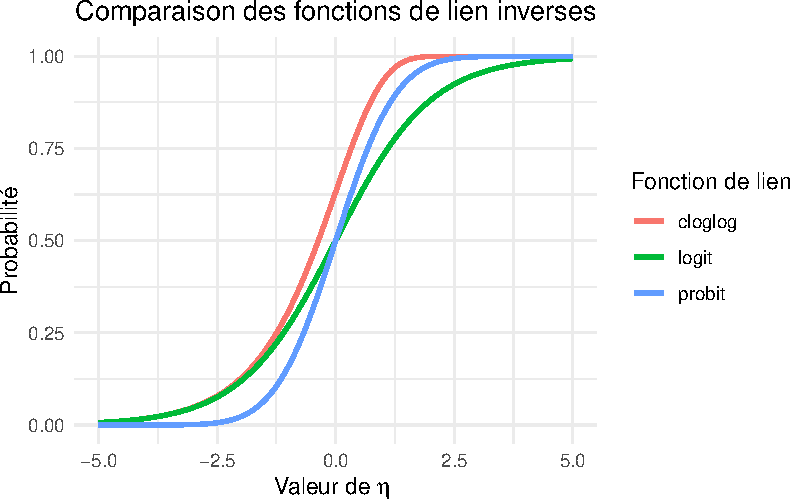
\includegraphics[keepaspectratio]{02-regression-logistique_files/figure-pdf/unnamed-chunk-1-1.pdf}}

\protect\phantomsection\label{sec-cotes}
{Le cas du lien logit --- Interprétation}

Avec le lien logit, on a

\[
\eta_i = \ln\left(\frac{\pi_i}{1-\pi_i}\right)
\]

et donc,

\[
e^{\eta_i} = \frac{\pi_i}{1-\pi_i}.
\]

{Définition --- Cote (odds)}

Le rapport ci-dessus a une interprétation concrète : c'est la cote
(\emph{odds}), notée \(o_i\) :

\[
o_i = \frac{\pi_i}{1-\pi_i} = \frac{P(Y_i=1)}{P(Y_i=0)}.
\]

Autrement dit, la cote compare la probabilité que l'événement se
produise (\(Y_i=1\)) à la probabilité qu'il ne se produise pas
(\(Y_i=0\)). Par exemple :

\begin{itemize}
\item
  si \(\pi_i = 0{,}5\), alors \(o_i = 1\) : autant de chances que
  l'événement arrive ou n'arrive pas ;
\item
  si \(\pi_i = 0{,}75\), alors \(o_i = 3\) : l'événement a 3 fois plus
  de chances de se produire que de ne pas se produire.
\end{itemize}

\textbf{Interprétation du coefficient \(\beta_j\).} Dans le modèle,

\[
\eta_i = \beta_0 + \beta_1 X_1 + \cdots + \beta_j X_j + \cdots
\]

Si on augmente \(X_j\) d'une unité, toutes les autres variables restant
constantes, \(\eta_i\) augmente de \(\beta_j\).

{Propriété --- Effet multiplicatif sur la cote}

Comme \(o_i = e^{\eta_i}\), une augmentation d'une unité de \(X_j\)
(toutes les autres variables restant constantes) se traduit par une
\emph{multiplication} de la cote :

\[
o_i^{\text{nouveau}} = e^{\eta_i + \beta_j} = e^{\eta_i} \cdot e^{\beta_j} = o_i^{\text{ancien}} \cdot e^{\beta_j}.
\]

Une augmentation unitaire de \(X_j\) multiplie donc la cote par
\(e^{\beta_j}\) ; \(e^{\beta_j}\) est le \textbf{rapport de cotes}
(\emph{odds ratio}). On distingue trois cas :

\begin{itemize}
\item
  si \(e^{\beta_j} > 1\) : augmenter \(X_j\) augmente la cote (et donc
  \(P(Y_i=1)\)) ;
\item
  si \(e^{\beta_j} < 1\) : augmenter \(X_j\) diminue la cote ;
\item
  si \(e^{\beta_j} = 1\) (c'est-à-dire \(\beta_j = 0\)) : \(X_j\) n'a
  pas d'effet sur la cote.
\end{itemize}

\section{Inférence statistique}\label{infuxe9rence-statistique-1}

\subsection{\texorpdfstring{Estimation des paramètres
\(\boldsymbol{\beta}\)}{Estimation des paramètres \textbackslash boldsymbol\{\textbackslash beta\}}}\label{estimation-des-paramuxe8tres-boldsymbolbeta}

\textbf{Point de départ : la vraisemblance.} On observe \(n\) variables
\(Y_i \sim \text{Binomiale}(m_i, \pi_i)\). La fonction de
log-vraisemblance s'écrit

\[
\ell(\boldsymbol{\pi}; \boldsymbol{y}) = \sum_{i=1}^n \log\left[P(Y_i = y_i)\right]
= \sum_{i=1}^n \left\{ \log\binom{m_i}{y_i} + y_i \log(\pi_i) + (m_i - y_i)\log(1-\pi_i) \right\}.
\]

\textbf{Lien avec \(\beta\).} Cette fonction dépend de \(\beta\)
\emph{indirectement}, via \(\pi_i\) : rappelons que

\[
\pi_i = g^{-1}(\beta_0 + \beta_1 X_{i1} + \cdots + \beta_p X_{ip}),
\]

où \(g^{-1}\) est l'inverse de la fonction de lien (par exemple la
fonction logistique si \(g\) est le lien logit).

\textbf{Reparamétrisation en termes de \(\mu_i\).} Il est parfois plus
commode de travailler avec \(\mu_i = m_i \pi_i\) (l'espérance de
\(Y_i\)) plutôt qu'avec \(\pi_i\) directement. En substituant
\(\pi_i = \mu_i/m_i\) dans la log-vraisemblance et en isolant tous les
termes qui ne dépendent pas de \(\beta\) (regroupés dans la constante
\(K\), qui contient le terme \(\log\binom{m_i}{y_i}\)), on obtient une
forme équivalente mais plus simple :

\[
\ell(\boldsymbol{\mu}; \boldsymbol{y}) = \sum_{i=1}^n \left\{ y_i \log(\mu_i) + (m_i - y_i)\log(m_i - \mu_i) \right\} + K,
\]

où \(\boldsymbol{\mu} = (\mu_1, \dots, \mu_n)^\top\) et \(K\) ne dépend
pas de \(\beta\) (donc n'affecte pas la maximisation). C'est sous cette
forme qu'on reconnaîtra, plus loin, que le modèle de régression
binomiale appartient à la famille exponentielle. Cette écriture est
aussi plus facile à utiliser pour le calcul de la
\hyperref[sec-deviance]{déviance}.

{Le cas du lien logit --- Log-vraisemblance}

Avec le lien logit, \(\pi_i = \dfrac{e^{\eta_i}}{1+e^{\eta_i}}\) et
\(1-\pi_i = \dfrac{1}{1+e^{\eta_i}}\), où

\[
\eta_i = \beta_0 + \beta_1 X_{i1} + \cdots + \beta_p X_{ip}.
\]

On a alors

\[
\log(\pi_i) = \eta_i - \log(1+e^{\eta_i}), \qquad \log(1-\pi_i) = -\log(1+e^{\eta_i}),
\]

de sorte que

\[
y_i \log(\pi_i) + (m_i - y_i)\log(1-\pi_i) = y_i \eta_i - m_i \log(1+e^{\eta_i}).
\]

La log-vraisemblance se réécrit donc directement en fonction de
\(\boldsymbol{\beta}\) :

\[
\ell(\boldsymbol{\beta}; \boldsymbol{y}) = \sum_{i=1}^n \left\{ \log\binom{m_i}{y_i} + y_i \eta_i - m_i \log\left(1+e^{\eta_i}\right) \right\}.
\]

\textbf{Estimation.} L'estimateur du maximum de vraisemblance
\(\hat{\boldsymbol{\beta}}\) est la valeur de \(\boldsymbol{\beta}\) qui
maximise \(\ell\). Contrairement à la régression linéaire classique, il
n'existe pas de solution analytique (forme fermée) ici, à cause de la
non-linéarité introduite par la fonction de lien \(g\). On doit donc
résoudre le problème numériquement, typiquement par l'algorithme des
moindres carrés pondérés itératifs (IRLS -- \emph{Iteratively Reweighted
Least Squares}), qui est une application de la méthode de Newton-Raphson
(ou Fisher scoring) à ce problème.

{Le cas du lien logit --- Estimation}

\textbf{Dérivée par rapport à \(\beta_j\)}

On dérive \(\ell(\boldsymbol{\beta}; \boldsymbol{y})\) terme à terme par
rapport à \(\beta_j\) (\(j = 0, 1, \dots, p\)), en notant que
\(\dfrac{\partial \eta_i}{\partial \beta_j} = X_{ij}\) (avec
\(X_{i0} \equiv 1\) pour l'ordonnée à l'origine).

Le terme \(\log\binom{m_i}{y_i}\) ne dépend pas de
\(\boldsymbol{\beta}\), sa dérivée est donc nulle. Pour le terme
\(y_i \eta_i\) :

\[
\frac{\partial}{\partial \beta_j}\left( y_i \eta_i \right) = y_i X_{ij}.
\]

Pour le terme \(m_i \log(1+e^{\eta_i})\), on utilise la règle de
dérivation en chaîne :

\[
\frac{\partial}{\partial \beta_j} \log\left(1+e^{\eta_i}\right)
= \frac{e^{\eta_i}}{1+e^{\eta_i}} \cdot \frac{\partial \eta_i}{\partial \beta_j}
= \pi_i X_{ij},
\]

d'où

\[
\frac{\partial}{\partial \beta_j}\left( m_i \log(1+e^{\eta_i}) \right) = m_i \pi_i X_{ij}.
\]

En combinant les trois morceaux, la dérivée partielle de la
log-vraisemblance est

\begin{equation}\protect\phantomsection\label{eq-score-logit}{
\frac{\partial \ell(\boldsymbol{\beta}; \boldsymbol{y})}{\partial \beta_j} = \sum_{i=1}^n \left( y_i - m_i \pi_i \right) X_{ij}.
}\end{equation}

\textbf{Vecteur score}

En posant
\(\boldsymbol{U}(\boldsymbol{\beta}) = \left( \dfrac{\partial \ell}{\partial \beta_0}, \dots, \dfrac{\partial \ell}{\partial \beta_p} \right)^\top\),
\(\boldsymbol{X}\) la matrice de design (\(n \times (p+1)\)),
\(\boldsymbol{y} = (y_1, \dots, y_n)^\top\) et
\(\boldsymbol{\mu} = (m_1\pi_1, \dots, m_n\pi_n)^\top\), on obtient sous
forme matricielle :

\begin{equation}\protect\phantomsection\label{eq-score-vecteur}{
\boldsymbol{U}(\boldsymbol{\beta}) = \boldsymbol{X}^\top (\boldsymbol{y} - \boldsymbol{\mu}).
}\end{equation}

\subsection{Séparation des données}\label{sec-separation}

{Définition --- Séparation complète et quasi-complète}

On dit qu'il y a \textbf{séparation complète} si un hyperplan permet de
classer parfaitement les \(Y_i\) à partir des covariables : il existe
\(\boldsymbol\beta\) tel que
\(\boldsymbol{X}_i^\top\boldsymbol\beta > 0\) chaque fois que \(Y_i=1\)
et \(\boldsymbol{X}_i^\top\boldsymbol\beta < 0\) chaque fois que
\(Y_i=0\) (ou l'inverse).

On parle de \textbf{séparation quasi-complète} lorsque cette séparation
est presque parfaite : il existe un hyperplan qui classe correctement
toutes les observations, sauf sur un sous-ensemble où
\(\boldsymbol{X}_i^\top\boldsymbol\beta = 0\) exactement.

En présence de séparation (complète ou quasi-complète), l'estimateur du
maximum de vraisemblance \(\hat{\boldsymbol\beta}\) \textbf{n'existe
pas} au sens usuel : la vraisemblance continue d'augmenter à mesure que
\(\|\boldsymbol\beta\| \to \infty\) dans la direction qui sépare les
données, sans jamais atteindre de maximum fini. En pratique,
l'algorithme IRLS ne converge pas, ou converge vers des \(\hat\beta_j\)
extrêmement grands, limités seulement par le critère d'arrêt numérique
de l'algorithme.

R signale souvent ce problème par l'avertissement

\begin{verbatim}
Warning: glm.fit: fitted probabilities numerically 0 or 1 occurred
\end{verbatim}

accompagné de coefficients estimés très grands en valeur absolue et
d'erreurs-types démesurément grandes --- souvent des ordres de grandeur
plus grandes que le coefficient lui-même.

{Exemple --- Illustration de la séparation complète}

\begin{Shaded}
\begin{Highlighting}[]
\FunctionTok{set.seed}\NormalTok{(}\DecValTok{1}\NormalTok{)}
\NormalTok{x }\OtherTok{\textless{}{-}} \FunctionTok{c}\NormalTok{(}\FunctionTok{rnorm}\NormalTok{(}\DecValTok{10}\NormalTok{, }\AttributeTok{mean =} \SpecialCharTok{{-}}\DecValTok{3}\NormalTok{), }\FunctionTok{rnorm}\NormalTok{(}\DecValTok{10}\NormalTok{, }\AttributeTok{mean =} \DecValTok{3}\NormalTok{))}
\NormalTok{y }\OtherTok{\textless{}{-}} \FunctionTok{c}\NormalTok{(}\FunctionTok{rep}\NormalTok{(}\DecValTok{0}\NormalTok{, }\DecValTok{10}\NormalTok{), }\FunctionTok{rep}\NormalTok{(}\DecValTok{1}\NormalTok{, }\DecValTok{10}\NormalTok{)) }\CommentTok{\# séparation complète : y=0 si x\textless{}0, y=1 si x\textgreater{}0}

\NormalTok{modele\_separe }\OtherTok{\textless{}{-}} \FunctionTok{glm}\NormalTok{(y }\SpecialCharTok{\textasciitilde{}}\NormalTok{ x, }\AttributeTok{family =}\NormalTok{ binomial)}
\end{Highlighting}
\end{Shaded}

\begin{verbatim}
Warning: glm.fit: algorithm did not converge
\end{verbatim}

\begin{verbatim}
Warning: glm.fit: fitted probabilities numerically 0 or 1 occurred
\end{verbatim}

\begin{Shaded}
\begin{Highlighting}[]
\FunctionTok{summary}\NormalTok{(modele\_separe)}\SpecialCharTok{$}\NormalTok{coefficients}
\end{Highlighting}
\end{Shaded}

\begin{verbatim}
             Estimate Std. Error      z value  Pr(>|z|)
(Intercept)  6.411375   36706.87 0.0001746642 0.9998606
x           20.668550   32170.73 0.0006424645 0.9994874
\end{verbatim}

\begin{Shaded}
\begin{Highlighting}[]
\FunctionTok{plot}\NormalTok{(x,y, }\AttributeTok{pch =} \DecValTok{19}\NormalTok{)}
\end{Highlighting}
\end{Shaded}

\pandocbounded{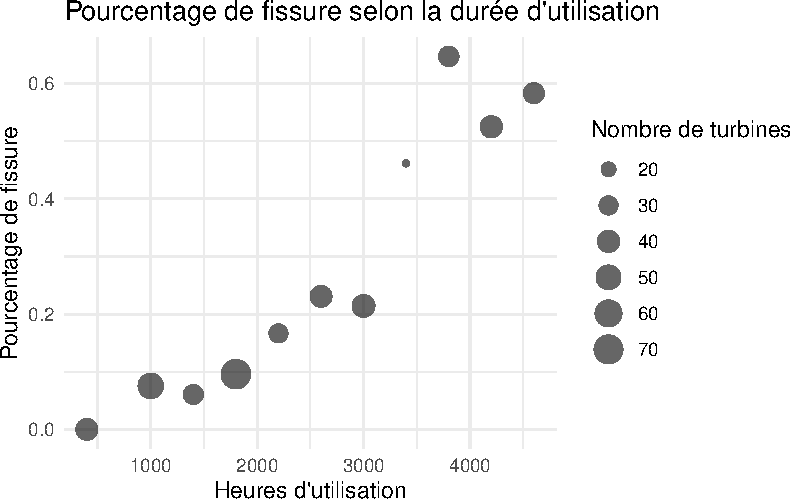
\includegraphics[keepaspectratio]{02-regression-logistique_files/figure-pdf/unnamed-chunk-2-1.pdf}}

Le coefficient de \texttt{x} et son erreur-type explosent tous les deux
--- signe clair de séparation, pas d'un effet réellement très fort.

{Remarque --- Que faire en cas de séparation?}

Quelques approches courantes :

\begin{itemize}
\tightlist
\item
  \textbf{Régression logistique pénalisée (Firth)} : ajoute un terme de
  pénalité à la vraisemblance (\texttt{logistf} en R), qui garantit
  l'existence d'un estimateur fini même sous séparation.
\item
  \textbf{Retirer ou regrouper la variable problématique} : si une
  variable catégorielle cause la séparation, fusionner la catégorie en
  cause avec une catégorie voisine peut régler le problème.
\item
  \textbf{Régularisation} (ridge, lasso) : contraint les coefficients et
  empêche qu'ils divergent vers l'infini.
\item
  \textbf{Recueillir plus de données} : si la séparation vient d'un
  petit échantillon plutôt que d'une relation déterministe réelle, un
  échantillon plus grand peut la faire disparaître.
\end{itemize}

Ce phénomène a aussi une conséquence directe sur l'inférence : les tests
de Wald deviennent peu fiables en présence de séparation, même partielle
--- voir le \hyperref[sec-hauckdonner]{phénomène de Hauck-Donner} plus
loin.

\subsection{Information de Fisher et variance des
estimateurs}\label{information-de-fisher-et-variance-des-estimateurs}

\textbf{Matrice d'information de Fisher.} On calcule ensuite la matrice
d'information de Fisher \(I\), dont l'élément \((j,k)\) est

\[
I_{jk} = -\left.\frac{\partial^2 \ell}{\partial \beta_j \partial \beta_k}\right|_{\hat{\boldsymbol{\beta}}}.
\]

La matrice de variance-covariance de \(\hb\) est estimée par

\[
\widehat{\text{Var}}(\hb) = I^{-1},
\]

et la distribution asymptotique de \(\hb\) est approximée par

\[
\hb \;\overset{\cdot}{\sim}\; \mathcal{N}\{\bb,\, \hvar{\hb} \}.
\]

\(\overset{\cdot}{\sim}\)

La notation \(\dot\sim\) signifie que la variable aléatoire suit
\emph{approximativement} la loi indiquée, de façon asymptotique --- ici,
quand \(n\to\infty\). Cette approximation provient d'un résultat de
convergence en distribution, qu'on explicitera à la
\hyperref[sec-deviance]{section sur la déviance}.

Dans ce qui suit, \(\hv{\hb}\) sera utilisé à la place de
\(\hvar{\hb}\), pour alléger la notation. De plus, on écrit
\(\hv{\hbj{j}}=[\hvar{\hb}]_{jj}\) quand on parle de la variance estimée
du paramètre \(\beta_j\).

\textbf{Forme explicite dans le cas binomial.} On montre que

\[
\widehat{\text{V}}(\hb)  = (X^\top W X)^{-1},
\]

où \(W\) est une matrice diagonale d'entrées

\[
w_i = \frac{\hmu{i} (m_i - \hmu{i})}{m_i},
\]

avec

\[
\hmu{i} = m_i \hpi{i} = m_i\, g^{-1}(\hbj{0} + \hbj{1} X_{i1} + \cdots + \hbj{p} X_{ip}).
\]

{Le cas du lien logit --- Expression de \(w_i\)}

\textbf{Remarque (Cas du lien logit).}

Avec le lien logit, \(\hpi{i} = \dfrac{e^{\heta{i}}}{1+e^{\heta{i}}}\),
où \(\heta{i} = \hbj{0} + \hbj{1} X_{i1} + \cdots + \hbj{p} X_{ip}\).
L'entrée \(w_i\) se simplifie alors en

\[
w_i = \frac{\hmu{i}(m_i - \hmu{i})}{m_i} = m_i\, \hpi{i}(1-\hpi{i}).
\]

{Exemple --- Jeu de données \hyperref[data-turbines]{\texttt{turbines}}}

On ajuste le modèle avec les trois fonctions de lien :

\begin{Shaded}
\begin{Highlighting}[]
\FunctionTok{library}\NormalTok{(GLMsData)}
\FunctionTok{data}\NormalTok{(turbines)}


\NormalTok{turbines\_obs }\OtherTok{\textless{}{-}}\NormalTok{ turbines }\SpecialCharTok{|\textgreater{}}
  \FunctionTok{mutate}\NormalTok{(}\AttributeTok{prop\_observee =}\NormalTok{ Fissures }\SpecialCharTok{/}\NormalTok{ Turbines)}

\FunctionTok{ggplot}\NormalTok{() }\SpecialCharTok{+}
  \FunctionTok{geom\_point}\NormalTok{(}
    \AttributeTok{data =}\NormalTok{ turbines\_obs,}
    \FunctionTok{aes}\NormalTok{(}\AttributeTok{x =}\NormalTok{ Hours, }\AttributeTok{y =}\NormalTok{ prop\_observee, }\AttributeTok{size =}\NormalTok{ Turbines),}
    \AttributeTok{color =} \StringTok{"black"}\NormalTok{,}
    \AttributeTok{alpha =} \FloatTok{0.6}
\NormalTok{  ) }\SpecialCharTok{+}
  \FunctionTok{labs}\NormalTok{(}
    \AttributeTok{x =} \StringTok{"Heures d\textquotesingle{}utilisation"}\NormalTok{,}
    \AttributeTok{y =} \StringTok{"Pourcentage de fissure"}\NormalTok{,}
    \AttributeTok{color =} \StringTok{"Fonction de lien"}\NormalTok{,}
    \AttributeTok{size =} \StringTok{"Nombre de turbines"}\NormalTok{,}
    \AttributeTok{title =} \StringTok{"Pourcentage de fissure selon la durée d\textquotesingle{}utilisation"}
\NormalTok{  ) }\SpecialCharTok{+}
  \FunctionTok{theme\_minimal}\NormalTok{()}
\end{Highlighting}
\end{Shaded}

\pandocbounded{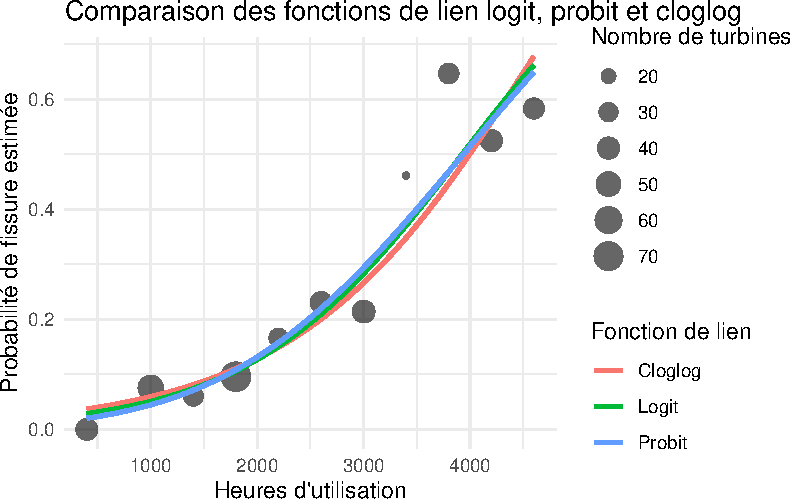
\includegraphics[keepaspectratio]{02-regression-logistique_files/figure-pdf/unnamed-chunk-3-1.pdf}}

\begin{Shaded}
\begin{Highlighting}[]
\NormalTok{modele.logit }\OtherTok{\textless{}{-}} \FunctionTok{glm}\NormalTok{(}
  \FunctionTok{cbind}\NormalTok{(Fissures, Turbines }\SpecialCharTok{{-}}\NormalTok{ Fissures) }\SpecialCharTok{\textasciitilde{}}\NormalTok{ Hours,}
  \AttributeTok{data =}\NormalTok{ turbines,}
  \AttributeTok{family =} \FunctionTok{binomial}\NormalTok{(}\AttributeTok{link =} \StringTok{"logit"}\NormalTok{)}
\NormalTok{)}
\NormalTok{modele.probit }\OtherTok{\textless{}{-}} \FunctionTok{glm}\NormalTok{(}
  \FunctionTok{cbind}\NormalTok{(Fissures, Turbines }\SpecialCharTok{{-}}\NormalTok{ Fissures) }\SpecialCharTok{\textasciitilde{}}\NormalTok{ Hours,}
  \AttributeTok{data =}\NormalTok{ turbines,}
  \AttributeTok{family =} \FunctionTok{binomial}\NormalTok{(}\AttributeTok{link =} \StringTok{"probit"}\NormalTok{)}
\NormalTok{)}
\NormalTok{modele.cloglog }\OtherTok{\textless{}{-}} \FunctionTok{glm}\NormalTok{(}
  \FunctionTok{cbind}\NormalTok{(Fissures, Turbines }\SpecialCharTok{{-}}\NormalTok{ Fissures) }\SpecialCharTok{\textasciitilde{}}\NormalTok{ Hours,}
  \AttributeTok{data =}\NormalTok{ turbines,}
  \AttributeTok{family =} \FunctionTok{binomial}\NormalTok{(}\AttributeTok{link =} \StringTok{"cloglog"}\NormalTok{)}
\NormalTok{)}
\FunctionTok{summary}\NormalTok{(modele.logit)}\SpecialCharTok{$}\NormalTok{coefficients}
\end{Highlighting}
\end{Shaded}

\begin{verbatim}
                 Estimate   Std. Error    z value     Pr(>|z|)
(Intercept) -3.9235965551 0.3779589447 -10.381013 3.025490e-25
Hours        0.0009992372 0.0001141505   8.753682 2.065015e-18
\end{verbatim}

\begin{Shaded}
\begin{Highlighting}[]
\FunctionTok{summary}\NormalTok{(modele.probit)}\SpecialCharTok{$}\NormalTok{coefficients}
\end{Highlighting}
\end{Shaded}

\begin{verbatim}
                 Estimate   Std. Error    z value     Pr(>|z|)
(Intercept) -2.2758074623 1.974187e-01 -11.527823 9.552869e-31
Hours        0.0005783211 6.259715e-05   9.238777 2.493310e-20
\end{verbatim}

\begin{Shaded}
\begin{Highlighting}[]
\FunctionTok{summary}\NormalTok{(modele.cloglog)}\SpecialCharTok{$}\NormalTok{coefficients}
\end{Highlighting}
\end{Shaded}

\begin{verbatim}
                 Estimate   Std. Error    z value     Pr(>|z|)
(Intercept) -3.6032798443 3.247391e-01 -11.095923 1.312978e-28
Hours        0.0008104936 9.013218e-05   8.992278 2.421587e-19
\end{verbatim}

\begin{Shaded}
\begin{Highlighting}[]
\FunctionTok{library}\NormalTok{(ggplot2)}
\FunctionTok{library}\NormalTok{(dplyr)}

\NormalTok{grille }\OtherTok{\textless{}{-}} \FunctionTok{data.frame}\NormalTok{(}
  \AttributeTok{Hours =} \FunctionTok{seq}\NormalTok{(}\FunctionTok{min}\NormalTok{(turbines}\SpecialCharTok{$}\NormalTok{Hours), }\FunctionTok{max}\NormalTok{(turbines}\SpecialCharTok{$}\NormalTok{Hours), }\AttributeTok{length.out =} \DecValTok{200}\NormalTok{)}
\NormalTok{)}

\NormalTok{predire\_modele }\OtherTok{\textless{}{-}} \ControlFlowTok{function}\NormalTok{(modele, nom\_lien) \{}
\NormalTok{  grille }\SpecialCharTok{|\textgreater{}}
    \FunctionTok{mutate}\NormalTok{(}
      \AttributeTok{p\_hat =} \FunctionTok{predict}\NormalTok{(modele, }\AttributeTok{newdata =}\NormalTok{ grille, }\AttributeTok{type =} \StringTok{"response"}\NormalTok{),}
      \AttributeTok{lien =}\NormalTok{ nom\_lien}
\NormalTok{    )}
\NormalTok{\}}

\NormalTok{predictions }\OtherTok{\textless{}{-}} \FunctionTok{bind\_rows}\NormalTok{(}
  \FunctionTok{predire\_modele}\NormalTok{(modele.logit, }\StringTok{"Logit"}\NormalTok{),}
  \FunctionTok{predire\_modele}\NormalTok{(modele.probit, }\StringTok{"Probit"}\NormalTok{),}
  \FunctionTok{predire\_modele}\NormalTok{(modele.cloglog, }\StringTok{"Cloglog"}\NormalTok{)}
\NormalTok{)}

\NormalTok{turbines\_obs }\OtherTok{\textless{}{-}}\NormalTok{ turbines }\SpecialCharTok{|\textgreater{}}
  \FunctionTok{mutate}\NormalTok{(}\AttributeTok{prop\_observee =}\NormalTok{ Fissures }\SpecialCharTok{/}\NormalTok{ Turbines)}

\FunctionTok{ggplot}\NormalTok{() }\SpecialCharTok{+}
  \FunctionTok{geom\_point}\NormalTok{(}
    \AttributeTok{data =}\NormalTok{ turbines\_obs,}
    \FunctionTok{aes}\NormalTok{(}\AttributeTok{x =}\NormalTok{ Hours, }\AttributeTok{y =}\NormalTok{ prop\_observee, }\AttributeTok{size =}\NormalTok{ Turbines),}
    \AttributeTok{color =} \StringTok{"black"}\NormalTok{,}
    \AttributeTok{alpha =} \FloatTok{0.6}
\NormalTok{  ) }\SpecialCharTok{+}
  \FunctionTok{geom\_line}\NormalTok{(}
    \AttributeTok{data =}\NormalTok{ predictions,}
    \FunctionTok{aes}\NormalTok{(}\AttributeTok{x =}\NormalTok{ Hours, }\AttributeTok{y =}\NormalTok{ p\_hat, }\AttributeTok{color =}\NormalTok{ lien),}
    \AttributeTok{linewidth =} \DecValTok{1}
\NormalTok{  ) }\SpecialCharTok{+}
  \FunctionTok{labs}\NormalTok{(}
    \AttributeTok{x =} \StringTok{"Heures d\textquotesingle{}utilisation"}\NormalTok{,}
    \AttributeTok{y =} \StringTok{"Probabilité de fissure estimée"}\NormalTok{,}
    \AttributeTok{color =} \StringTok{"Fonction de lien"}\NormalTok{,}
    \AttributeTok{size =} \StringTok{"Nombre de turbines"}\NormalTok{,}
    \AttributeTok{title =} \StringTok{"Comparaison des fonctions de lien logit, probit et cloglog"}
\NormalTok{  ) }\SpecialCharTok{+}
  \FunctionTok{theme\_minimal}\NormalTok{()}
\end{Highlighting}
\end{Shaded}

\pandocbounded{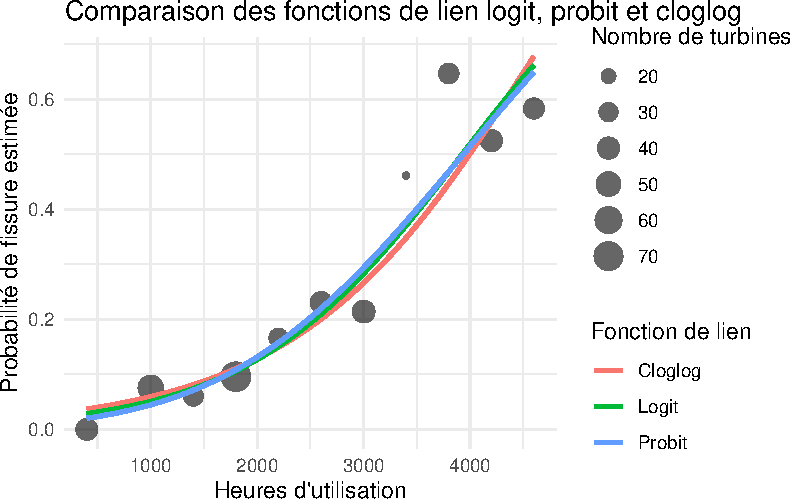
\includegraphics[keepaspectratio]{02-regression-logistique_files/figure-pdf/unnamed-chunk-4-1.pdf}}

Les trois liens mènent à des coefficients significatifs et à des courbes
prédites \(\hat\pi^*\) très similaires.

Les intervalles de confiance et tests concernant les \(\beta_j\) sont
obtenus par la méthode de \textbf{Wald}. Un intervalle de confiance de
niveau \((1-\alpha)\) pour \(\beta_j\) est
\[\left[\hat\beta_j - z_{\alpha/2}\sqrt{\hat{\text V}(\hat\beta_j)}\,;\ \hat\beta_j + z_{\alpha/2}\sqrt{\hat{\text V}(\hat\beta_j)}\right],\]
où \(z_\gamma\) est le quantile de la \(\mathcal{N}(0,1)\) défini par
\(P(Z > z_\gamma) = \gamma\).

Pour tester \(H_0: \beta_j = 0\) contre \(H_1: \beta_j\neq 0\), on
rejette \(H_0\) au seuil \(\alpha\) si \(|z_{obs}| > z_{\alpha/2}\),
avec \(z_{obs} = \hat\beta_j/\sqrt{\hat{\text V}(\hat\beta_j)}\). Le
seuil observé (\(p\)-valeur) est \(\alpha^* = 2P(Z > |z_{obs}|)\).

\protect\phantomsection\label{sec-hauckdonner}
{Remarque --- Le phénomène de Hauck-Donner}

Le test de Wald pour \(H_0 : \beta_j = 0\) repose sur la statistique

\[
z_{obs} = \frac{\hat\beta_j}{\sqrt{\hat{\text V}(\hat\beta_j)}},
\]

où l'erreur-type est estimée à partir de la courbure de la
log-vraisemblance \textbf{évaluée au point estimé} \(\hat\beta_j\),
plutôt que sous \(H_0\). Cette dépendance locale peut mener à un
comportement contre-intuitif : lorsque \(|\hat\beta_j|\) devient très
grand (par exemple en présence de \hyperref[sec-separation]{séparation}
--- complète ou quasi-complète --- ou d'un effet très fort), la courbure
de la vraisemblance en \(\hat\beta_j\) s'aplatit, ce qui \textbf{gonfle}
\(\sqrt{\hat{\text V}(\hat\beta_j)}\) et peut faire \textbf{diminuer}
\(z_{obs}\) --- donnant l'impression que l'effet n'est pas significatif,
alors qu'il l'est. On pourrait montrer que cela est causé par le fait
que l'erreur-type augmente plus rapidement que la valeur absolue de
l'estimation du paramètre.

Ce phénomène, documenté par Hauck et Donner (1977), n'affecte pas le
test du rapport de vraisemblance, qui compare directement la
vraisemblance en \(\hat\beta_j\) à celle en \(0\) plutôt que de
s'appuyer sur une approximation locale :

\[
G^2 = -2\left[\ell(\text{modèle réduit}) - \ell(\text{modèle complet})\right] \;\overset{\cdot}{\sim}\; \chi^2_1 \quad \text{sous } H_0.
\]

\textbf{En pratique} : le test «par défaut» de la plupart des fonctions
de R utilise le test de Wald, car celui-ci est moins coûteux en calcul
et est fiable avec de grands échantillons. Il faut porter une attention
particulière aux cas où un coefficient très grand ressort avec une
valeur-p de Wald étonnamment élevée. Il faut comparer avec
\texttt{anova(modele\_reduit,\ modele\_complet,\ test\ =\ "Chisq")}
avant de conclure à la non-significativité.

{Exemple --- Effet Hauck-Donner}

\begin{Shaded}
\begin{Highlighting}[]
\FunctionTok{library}\NormalTok{(purrr)}
\FunctionTok{library}\NormalTok{(dplyr)}
\FunctionTok{library}\NormalTok{(ggplot2)}

\NormalTok{simuler\_logistique }\OtherTok{\textless{}{-}} \ControlFlowTok{function}\NormalTok{(n, }\AttributeTok{beta0 =} \DecValTok{0}\NormalTok{, }\AttributeTok{beta1 =} \DecValTok{1}\NormalTok{) \{}
\NormalTok{  x }\OtherTok{\textless{}{-}} \FunctionTok{rnorm}\NormalTok{(n, }\AttributeTok{mean =} \DecValTok{0}\NormalTok{, }\AttributeTok{sd =} \DecValTok{1}\NormalTok{)}
\NormalTok{  eta }\OtherTok{\textless{}{-}}\NormalTok{ beta0 }\SpecialCharTok{+}\NormalTok{ beta1 }\SpecialCharTok{*}\NormalTok{ x}
\NormalTok{  p }\OtherTok{\textless{}{-}} \FunctionTok{plogis}\NormalTok{(eta)}
\NormalTok{  y }\OtherTok{\textless{}{-}} \FunctionTok{rbinom}\NormalTok{(n, }\AttributeTok{size =} \DecValTok{1}\NormalTok{, }\AttributeTok{prob =}\NormalTok{ p)}
  \FunctionTok{data.frame}\NormalTok{(}\AttributeTok{x =}\NormalTok{ x, }\AttributeTok{y =}\NormalTok{ y)}
\NormalTok{\}}

\FunctionTok{set.seed}\NormalTok{(}\DecValTok{123}\NormalTok{)}
\NormalTok{n }\OtherTok{\textless{}{-}} \DecValTok{200}
\NormalTok{valeurs\_beta1 }\OtherTok{\textless{}{-}} \FunctionTok{seq}\NormalTok{(}\FloatTok{0.5}\NormalTok{, }\DecValTok{15}\NormalTok{, }\AttributeTok{by =} \FloatTok{0.5}\NormalTok{) }\CommentTok{\# vrai effet croissant {-}\textgreater{} séparation}

\NormalTok{resultats }\OtherTok{\textless{}{-}} \FunctionTok{map\_dfr}\NormalTok{(valeurs\_beta1, }\ControlFlowTok{function}\NormalTok{(b1) \{}
\NormalTok{  dat }\OtherTok{\textless{}{-}} \FunctionTok{simuler\_logistique}\NormalTok{(n, }\AttributeTok{beta0 =} \DecValTok{0}\NormalTok{, }\AttributeTok{beta1 =}\NormalTok{ b1)}

\NormalTok{  mod\_complet }\OtherTok{\textless{}{-}} \FunctionTok{glm}\NormalTok{(y }\SpecialCharTok{\textasciitilde{}}\NormalTok{ x, }\AttributeTok{data =}\NormalTok{ dat, }\AttributeTok{family =}\NormalTok{ binomial)}
\NormalTok{  mod\_reduit }\OtherTok{\textless{}{-}} \FunctionTok{glm}\NormalTok{(y }\SpecialCharTok{\textasciitilde{}} \DecValTok{1}\NormalTok{, }\AttributeTok{data =}\NormalTok{ dat, }\AttributeTok{family =}\NormalTok{ binomial)}

\NormalTok{  beta\_hat }\OtherTok{\textless{}{-}} \FunctionTok{coef}\NormalTok{(mod\_complet)[}\StringTok{"x"}\NormalTok{]}
\NormalTok{  et\_hat }\OtherTok{\textless{}{-}} \FunctionTok{summary}\NormalTok{(mod\_complet)}\SpecialCharTok{$}\NormalTok{coefficients[}\StringTok{"x"}\NormalTok{, }\StringTok{"Std. Error"}\NormalTok{]}
\NormalTok{  wald\_chisq }\OtherTok{\textless{}{-}}\NormalTok{ (beta\_hat }\SpecialCharTok{/}\NormalTok{ et\_hat)}\SpecialCharTok{\^{}}\DecValTok{2}
\NormalTok{  lr\_chisq }\OtherTok{\textless{}{-}} \FunctionTok{as.numeric}\NormalTok{(}\DecValTok{2} \SpecialCharTok{*}\NormalTok{ (}\FunctionTok{logLik}\NormalTok{(mod\_complet) }\SpecialCharTok{{-}} \FunctionTok{logLik}\NormalTok{(mod\_reduit)))}

  \FunctionTok{data.frame}\NormalTok{(}
    \AttributeTok{beta1\_vrai =}\NormalTok{ b1,}
    \AttributeTok{beta\_hat =}\NormalTok{ beta\_hat,}
    \AttributeTok{wald\_chisq =}\NormalTok{ wald\_chisq,}
    \AttributeTok{lr\_chisq =}\NormalTok{ lr\_chisq}
\NormalTok{  )}
\NormalTok{\})}

\NormalTok{resultats }\SpecialCharTok{|\textgreater{}}
\NormalTok{  tidyr}\SpecialCharTok{::}\FunctionTok{pivot\_longer}\NormalTok{(}
    \FunctionTok{c}\NormalTok{(wald\_chisq, lr\_chisq),}
    \AttributeTok{names\_to =} \StringTok{"test"}\NormalTok{,}
    \AttributeTok{values\_to =} \StringTok{"statistique"}
\NormalTok{  ) }\SpecialCharTok{|\textgreater{}}
  \FunctionTok{mutate}\NormalTok{(}
    \AttributeTok{test =} \FunctionTok{recode}\NormalTok{(}
\NormalTok{      test,}
      \AttributeTok{wald\_chisq =} \StringTok{"Wald (khi{-}carré)"}\NormalTok{,}
      \AttributeTok{lr\_chisq =} \StringTok{"Rapport de vraisemblance"}
\NormalTok{    )}
\NormalTok{  ) }\SpecialCharTok{|\textgreater{}}
  \FunctionTok{ggplot}\NormalTok{(}\FunctionTok{aes}\NormalTok{(}\AttributeTok{x =}\NormalTok{ beta\_hat, }\AttributeTok{y =}\NormalTok{ statistique, }\AttributeTok{color =}\NormalTok{ test)) }\SpecialCharTok{+}
  \FunctionTok{geom\_line}\NormalTok{(}\AttributeTok{linewidth =} \DecValTok{1}\NormalTok{) }\SpecialCharTok{+}
  \FunctionTok{labs}\NormalTok{(}
    \AttributeTok{x =} \FunctionTok{expression}\NormalTok{(}\FunctionTok{hat}\NormalTok{(beta)[x]),}
    \AttributeTok{y =} \StringTok{"Statistique de test (échelle khi{-}carré, 1 ddl)"}\NormalTok{,}
    \AttributeTok{color =} \ConstantTok{NULL}\NormalTok{,}
    \AttributeTok{title =} \StringTok{"Effet Hauck{-}Donner avec un prédicteur continu"}
\NormalTok{  ) }\SpecialCharTok{+}
  \FunctionTok{theme\_minimal}\NormalTok{()}
\end{Highlighting}
\end{Shaded}

\pandocbounded{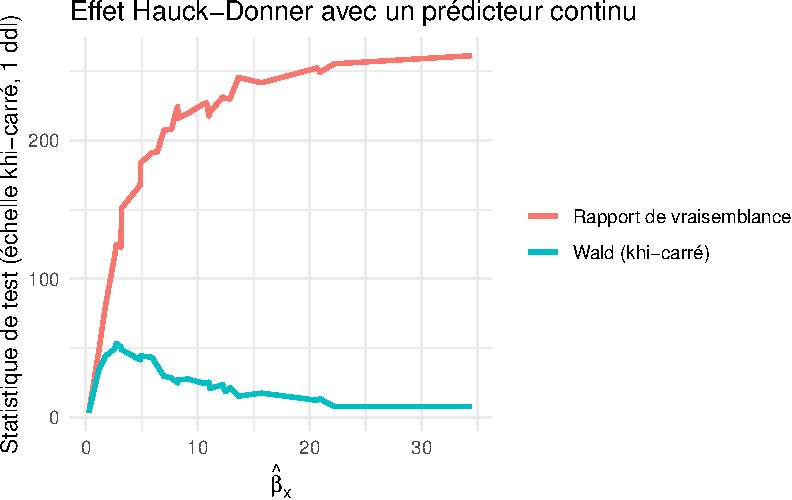
\includegraphics[keepaspectratio]{02-regression-logistique_files/figure-pdf/hauck-donner-sim-continu-1.pdf}}

\subsection{Comparaison directe des
sorties}\label{comparaison-directe-des-sorties}

Pour illustrer concrètement l'écart entre les deux tests, comparons un
cas ``normal'' (\(k = 15\), pas de séparation) à un cas de séparation
quasi-complète (\(k = 19\), un seul échec sur 20 dans le groupe
\(x = 1\)) :

\begin{Shaded}
\begin{Highlighting}[]
\NormalTok{simuler\_logistique }\OtherTok{\textless{}{-}} \ControlFlowTok{function}\NormalTok{(n, }\AttributeTok{beta0 =} \DecValTok{0}\NormalTok{, }\AttributeTok{beta1 =} \DecValTok{1}\NormalTok{) \{}
\NormalTok{  x }\OtherTok{\textless{}{-}} \FunctionTok{rnorm}\NormalTok{(n, }\AttributeTok{mean =} \DecValTok{0}\NormalTok{, }\AttributeTok{sd =} \DecValTok{1}\NormalTok{)}
\NormalTok{  eta }\OtherTok{\textless{}{-}}\NormalTok{ beta0 }\SpecialCharTok{+}\NormalTok{ beta1 }\SpecialCharTok{*}\NormalTok{ x}
\NormalTok{  p }\OtherTok{\textless{}{-}} \FunctionTok{plogis}\NormalTok{(eta) }\CommentTok{\# équivalent à 1 / (1 + exp({-}eta))}
\NormalTok{  y }\OtherTok{\textless{}{-}} \FunctionTok{rbinom}\NormalTok{(n, }\AttributeTok{size =} \DecValTok{1}\NormalTok{, }\AttributeTok{prob =}\NormalTok{ p)}
  \FunctionTok{data.frame}\NormalTok{(}\AttributeTok{x =}\NormalTok{ x, }\AttributeTok{y =}\NormalTok{ y)}
\NormalTok{\}}

\CommentTok{\# Cas 1 : k = 15, pas de séparation}
\NormalTok{dat\_normal }\OtherTok{\textless{}{-}} \FunctionTok{simuler\_logistique}\NormalTok{(}\AttributeTok{n =} \DecValTok{50}\NormalTok{, }\AttributeTok{beta0 =} \DecValTok{0}\NormalTok{, }\AttributeTok{beta1 =} \DecValTok{5}\NormalTok{)}

\FunctionTok{plot}\NormalTok{(dat\_normal}\SpecialCharTok{$}\NormalTok{x, dat\_normal}\SpecialCharTok{$}\NormalTok{y)}
\end{Highlighting}
\end{Shaded}

\pandocbounded{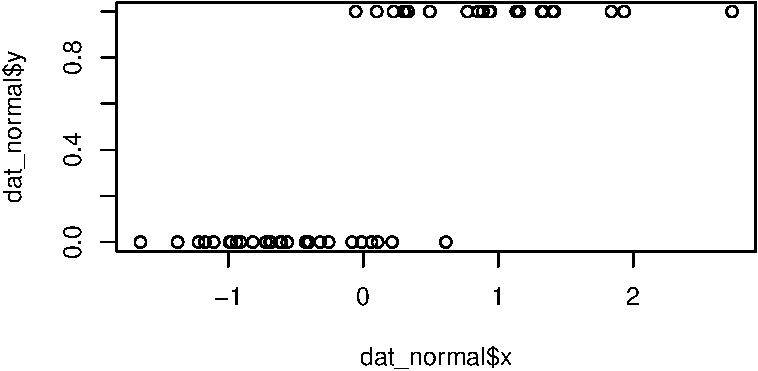
\includegraphics[keepaspectratio]{02-regression-logistique_files/figure-pdf/hauck-donner-exemples-1.pdf}}

\begin{Shaded}
\begin{Highlighting}[]
\NormalTok{mod\_normal }\OtherTok{\textless{}{-}} \FunctionTok{glm}\NormalTok{(y }\SpecialCharTok{\textasciitilde{}}\NormalTok{ x, }\AttributeTok{data =}\NormalTok{ dat\_normal, }\AttributeTok{family =}\NormalTok{ binomial)}
\FunctionTok{summary}\NormalTok{(mod\_normal)}\SpecialCharTok{$}\NormalTok{coefficients}
\end{Highlighting}
\end{Shaded}

\begin{verbatim}
              Estimate Std. Error   z value    Pr(>|z|)
(Intercept) -0.9870555  0.6429306 -1.535244 0.124723837
x            5.7141805  1.9696783  2.901073 0.003718873
\end{verbatim}

\begin{Shaded}
\begin{Highlighting}[]
\CommentTok{\# Cas 2 : k = 19, séparation quasi{-}complète}
\FunctionTok{set.seed}\NormalTok{(}\DecValTok{1234}\NormalTok{)}
\NormalTok{dat\_separe }\OtherTok{\textless{}{-}} \FunctionTok{simuler\_logistique}\NormalTok{(}\AttributeTok{n =} \DecValTok{50}\NormalTok{, }\AttributeTok{beta0 =} \DecValTok{0}\NormalTok{, }\AttributeTok{beta1 =} \DecValTok{15}\NormalTok{)}

\FunctionTok{plot}\NormalTok{(dat\_separe}\SpecialCharTok{$}\NormalTok{x, dat\_separe}\SpecialCharTok{$}\NormalTok{y)}
\end{Highlighting}
\end{Shaded}

\pandocbounded{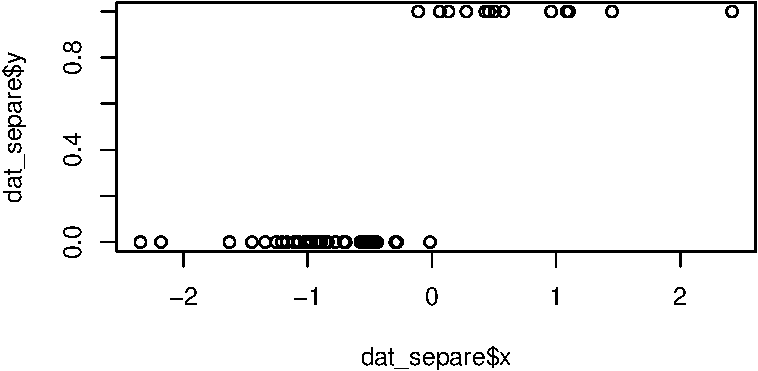
\includegraphics[keepaspectratio]{02-regression-logistique_files/figure-pdf/hauck-donner-exemples-2.pdf}}

\begin{Shaded}
\begin{Highlighting}[]
\NormalTok{mod\_separe }\OtherTok{\textless{}{-}} \FunctionTok{glm}\NormalTok{(y }\SpecialCharTok{\textasciitilde{}}\NormalTok{ x, }\AttributeTok{data =}\NormalTok{ dat\_separe, }\AttributeTok{family =}\NormalTok{ binomial)}
\FunctionTok{summary}\NormalTok{(mod\_separe)}\SpecialCharTok{$}\NormalTok{coefficients}
\end{Highlighting}
\end{Shaded}

\begin{verbatim}
             Estimate Std. Error   z value  Pr(>|z|)
(Intercept)  1.028036   1.301805 0.7897003 0.4297028
x           14.144188   7.929599 1.7837205 0.0744691
\end{verbatim}

On constate ici que la valeur-p n'est pas significative au seuil 5\%.

Si on regarde les valeurs-p des tests des rapports de vraisemblance pour
les deux cas:

\begin{Shaded}
\begin{Highlighting}[]
\NormalTok{mod\_normal\_reduit }\OtherTok{\textless{}{-}} \FunctionTok{glm}\NormalTok{(y }\SpecialCharTok{\textasciitilde{}} \DecValTok{1}\NormalTok{, }\AttributeTok{data =}\NormalTok{ dat\_normal, }\AttributeTok{family =}\NormalTok{ binomial)}
\FunctionTok{anova}\NormalTok{(mod\_normal\_reduit, mod\_normal, }\AttributeTok{test =} \StringTok{"Chisq"}\NormalTok{)}
\end{Highlighting}
\end{Shaded}

\begin{verbatim}
Analysis of Deviance Table

Model 1: y ~ 1
Model 2: y ~ x
  Resid. Df Resid. Dev Df Deviance  Pr(>Chi)    
1        49     68.593                          
2        48     19.252  1   49.341 2.151e-12 ***
---
Signif. codes:  0 '***' 0.001 '**' 0.01 '*' 0.05 '.' 0.1 ' ' 1
\end{verbatim}

\begin{Shaded}
\begin{Highlighting}[]
\NormalTok{mod\_separe\_reduit }\OtherTok{\textless{}{-}} \FunctionTok{glm}\NormalTok{(y }\SpecialCharTok{\textasciitilde{}} \DecValTok{1}\NormalTok{, }\AttributeTok{data =}\NormalTok{ dat\_separe, }\AttributeTok{family =}\NormalTok{ binomial)}
\FunctionTok{anova}\NormalTok{(mod\_separe\_reduit, mod\_separe, }\AttributeTok{test =} \StringTok{"Chisq"}\NormalTok{)}
\end{Highlighting}
\end{Shaded}

\begin{verbatim}
Analysis of Deviance Table

Model 1: y ~ 1
Model 2: y ~ x
  Resid. Df Resid. Dev Df Deviance  Pr(>Chi)    
1        49     57.306                          
2        48      4.990  1   52.316 4.725e-13 ***
---
Signif. codes:  0 '***' 0.001 '**' 0.01 '*' 0.05 '.' 0.1 ' ' 1
\end{verbatim}

\subsection{Intervalle de confiance pour une probabilité
prédite}\label{intervalle-de-confiance-pour-une-probabilituxe9-pruxe9dite}

Pour \(\boldsymbol{X}^* = (1, X_1^*,\ldots,X_p^*)^\top\), on estime
\(\pi^*\) par \(\hat\pi^* = g^{-1}({\boldsymbol{X}^*}^\top\hat\beta)\).
Deux approches :

\begin{enumerate}
\def\labelenumi{\arabic{enumi}.}
\item
  \textbf{Transformation de l'intervalle sur \(\eta^*\)} : un IC pour
  \({X^*}^\top\beta\) est
  \[\left[{\boldsymbol{X}^*}^\top\hat\beta \pm z_{\alpha/2}\sqrt{\hat{\text V}({\boldsymbol{X}^*}^\top\hat\beta)}\right], \qquad \hat{\text V}({\boldsymbol{X}^*}^\top\hat\beta) = {\boldsymbol{X}^*}^\top \hat{\text V}(\hat\beta)\, \boldsymbol{X}^*,\]
  et on applique \(g^{-1}\) aux deux bornes. Cet intervalle respecte
  toujours \([0,1]\).
\item
  \textbf{Méthode du delta} :
  \(\hat{\text V}(\hat\pi^*) = h({\boldsymbol{X}^*}^\top\hat\beta)\, \hat{\text V}({\boldsymbol{X}^*}^\top\hat\beta)\)
  avec \(h(u) = \{\partial g^{-1}(u)/\partial u\}^2\), d'où l'IC
  approximatif
  \(\left[\hat\pi^* \pm z_{\alpha/2}\sqrt{\hat{\text V}(\hat\pi^*)}\right]\).
\end{enumerate}

Les deux méthodes donnent en pratique des résultats très similaires.

{Le cas du lien logit --- Méthode du delta}

Avec le lien logit, \(g^{-1}(u) = \dfrac{e^u}{1+e^u}\), dont la dérivée
est

\[
\frac{\partial g^{-1}(u)}{\partial u} = \frac{e^u}{(1+e^u)^2} = g^{-1}(u)\left\{1-g^{-1}(u)\right\}.
\]

Ainsi, \(h(u) = \left[g^{-1}(u)\{1-g^{-1}(u)\}\right]^2\), et évalué en
\(u = {\boldsymbol{X}^*}^\top\hat\beta\), on obtient
\(h({\boldsymbol{X}^*}^\top\hat\beta) = \left[\hat\pi^*(1-\hat\pi^*)\right]^2\).
La règle du delta donne alors

\[
\hat{\text V}(\hat\pi^*) = \left[\hat\pi^*(1-\hat\pi^*)\right]^2 \hat{\text V}\left({\boldsymbol{X}^*}^\top\hat\beta\right).
\]

{Pour aller plus loin avec la théorie --- Idée de la méthode du delta}

On a \(\hat\theta = {\boldsymbol{X}^*}^\top\hat\beta\), dont on connaît
la distribution asymptotique :
\(\hat\theta \overset{\cdot}{\sim} \mathcal{N}(\theta,\, \hat{\text V}(\hat\theta))\).
On s'intéresse cependant à \(\hat\pi^* = g^{-1}(\hat\theta)\), une
transformation \emph{non linéaire} de \(\hat\theta\) --- et la normalité
asymptotique ne se transporte pas automatiquement à travers une
transformation non linéaire, ni sa variance.

La méthode du delta contourne le problème en approximant \(g^{-1}\)
localement par sa tangente (développement de Taylor au premier ordre)
autour de \(\theta\) : \[
g^{-1}(\hat\theta) \approx g^{-1}(\theta) + \left.\frac{\partial g^{-1}(u)}{\partial u}\right|_{u=\theta} (\hat\theta - \theta).
\] Comme \(g^{-1}(\theta) = \pi^*\) est une constante et que le second
terme n'est qu'une transformation \emph{linéaire} de \(\hat\theta\), on
peut maintenant calculer sa variance directement : \[
\text{Var}(\hat\pi^*) \approx \left[\left.\frac{\partial g^{-1}(u)}{\partial u}\right|_{u=\theta}\right]^2 \text{Var}(\hat\theta),
\] qu'on estime en substituant \(\hat\theta\) à \(\theta\) (d'où
\(\hat{\text V}(\hat\pi^*) = h({\boldsymbol{X}^*}^\top\hat\beta)\,\hat{\text V}({\boldsymbol{X}^*}^\top\hat\beta)\),
où \(h(u) = \{\partial g^{-1}(u)/\partial u\}^2\)).

Contrairement à la première approche (transformer les bornes de l'IC sur
\(\eta^*\)), cette méthode approxime directement la variance de
\(\hat\pi^*\) sur son échelle naturelle --- mais comme elle repose sur
une approximation linéaire locale, l'intervalle de confiance qui en
résulte n'est pas garanti de rester dans \([0,1]\), contrairement à
celui obtenu par transformation.

\section{Sélection de modèles}\label{suxe9lection-de-moduxe8les}

\subsection{Déviance}\label{sec-deviance}

Pour juger si un modèle avec \(p+1\) paramètres \(\boldsymbol\beta\)
s'ajuste bien aux données, il est utile de le comparer au modèle le plus
flexible possible : celui qui accorde à chaque observation son propre
paramètre, sans aucune structure imposée par des variables explicatives.

{Définition --- Modèle saturé}

On l'appelle le \textbf{modèle saturé}, avec \(n\) paramètres
\(\{\tilde\mu_1,\ldots,\tilde\mu_n\}\) (un par observation, plutôt que
\(p+1\) pour l'ensemble de l'échantillon).

Il est facile de constater que le modèle saturé maximise la
log-vraisemblance, donnée par \[
\ell(\tilde\mu_1,\ldots,\tilde\mu_n; \boldsymbol{y}) = \sum_{i=1}^n \left\{ y_i \log(\tilde\mu_i) + (m_i - y_i)\log(m_i - \tilde\mu_i) \right\} + K,
\]

quand \(\{\tilde\mu_1,\ldots,\tilde\mu_n\}= \{y_1,\ldots,y_n\}\),
c'est-à-dire si la log-vraisemblance est calculée en ajustant chaque
paramètre exactement sur la donnée observée correspondante. Le modèle
saturé représente donc l'ajustement \emph{parfait} : il reproduit
exactement les données, sans laisser aucun résidu. Il n'a cependant
aucune valeur prédictive ou explicative, puisqu'il ne fait que mémoriser
les observations --- son seul rôle est de servir de référence, un étalon
auquel comparer un modèle plus parcimonieux (avec \(p+1 \ll n\)
paramètres) pour quantifier ce qui reste à expliquer.

\textbf{La déviance.} En notant
\(\tilde{\boldsymbol{\mu}}=(\tilde\mu_1,\ldots,\tilde\mu_n)^\top\) et
\(\hat{\boldsymbol{\mu}}=(\hat\mu_1,\ldots,\hat\mu_n)^\top\), la
statistique du rapport de vraisemblance entre le modèle saturé et le
modèle considéré est

\[\Lambda=\frac{L(\tilde{\boldsymbol{\mu}}; \boldsymbol y)}{L(\hat{\boldsymbol{\mu}}; \boldsymbol y)} =\frac{L(\boldsymbol{y}; \boldsymbol y)}{L(\hat{\boldsymbol{\mu}}; \boldsymbol y)}.\]

{Définition --- Déviance}

On définit la déviance \(D\) comme étant deux fois le log de ce rapport:

\[D =2\left\{l(y,y) - l(\hat\mu,y)\right\} = 2\sum_{i=1}^n\left\{y_i\log\!\left(\frac{y_i}{\hmu{i}}\right) + (m_i - y_i)\log\!\left(\frac{m_i - y_i}{m_i - \hmu{i}}\right)\right\} = \sum_{i=1}^n d_i.\]

\(D\) est la \textbf{déviance} du modèle et \(d_i\) la déviance
individuelle de l'observation \(i\) ; chaque \(d_i\) mesure l'écart
entre l'ajustement parfait \(y_i\) et l'ajustement \(\hmu{i}\) obtenu
par le modèle.

{Remarque}

Le \(2\) de la formule de la déviance est nécessaire pour avoir

\[D \xrightarrow{d} \chi_{n-(p+1)}^2, \text{lorsque } m_i\to \infty,\]

c'est-à-dire que la déviance tend vers la loi du khi-carré à \(n-(p+1)\)
degrés de liberté quand les \(m_i\) tendent vers l'infini.

\(\xrightarrow{d}\)

La flèche \(\xrightarrow{d}\) indique une \textbf{convergence en
distribution} (ou en loi) : la distribution de la quantité à gauche (ici
\(D\)) se rapproche de celle indiquée à droite (ici
\(\chi^2_{n-(p+1)}\)) lorsque le paramètre asymptotique tend vers
l'infini (ici \(m_i\)), sans que \(D\) elle-même ne converge vers une
valeur précise. C'est ce même type de convergence qui justifiait la
notation \(\dot\sim\) utilisée plus tôt pour \(\hat\beta\).

Autrement, c'est-à-dire lorsque les \(m_i\) sont finis, on utilise
plutôt

\[D \;\overset{\cdot}{\sim}\; \chi_{n-(p+1)}^2\]

comme approximation.

{Propriété --- Non-négativité de la déviance}

Puisque le modèle saturé maximise la vraisemblance parmi \emph{tous} les
modèles possibles, \(l(y,y) \geq l(\hat\mu,y)\) toujours, et donc
\(D \geq 0\) : plus \(D\) est petit, plus le modèle considéré se
rapproche du modèle saturé, donc plus il s'ajuste bien aux données.

La déviance joue le même rôle que la somme des carrés des résidus en
régression linéaire : elle sert à évaluer l'adéquation du modèle et à
comparer des modèles.

\subsection{Comparaison de modèles
emboîtés}\label{comparaison-de-moduxe8les-embouxeetuxe9s}

Pour comparer deux modèles emboîtés de déviances \(D_1\) (complet) et
\(D_2\) (réduit), la statistique de test est \(\chi^2 = D_2 - D_1\).

{Propriété --- Distribution asymptotique de \(\chi^2 = D_2-D_1\)}

Sous \(H_0\) (le modèle réduit est adéquat), \(\chi^2\) suit une loi du
khi-deux à \(d\) degrés de liberté, où \(d\) est la différence du nombre
de paramètres.

{Exemple --- Introduction des termes quadratiques et cubiques dans
l'exemple \hyperref[data-turbines]{\texttt{turbines}}}

On teste \(H_0: \beta_2 = \beta_3 = 0\) (modèle avec \texttt{Hours}
seulement contre modèle avec termes en \texttt{Hours}\(^2\) et
\texttt{Hours}\(^3\)) :

\begin{Shaded}
\begin{Highlighting}[]
\FunctionTok{library}\NormalTok{(GLMsData)}
\FunctionTok{data}\NormalTok{(turbines)}

\NormalTok{modele.reduit }\OtherTok{\textless{}{-}} \FunctionTok{glm}\NormalTok{(}
  \FunctionTok{cbind}\NormalTok{(Fissures, Turbines }\SpecialCharTok{{-}}\NormalTok{ Fissures) }\SpecialCharTok{\textasciitilde{}}\NormalTok{ Hours,}
  \AttributeTok{data =}\NormalTok{ turbines,}
  \AttributeTok{family =}\NormalTok{ binomial}
\NormalTok{)}
\NormalTok{modele.complet }\OtherTok{\textless{}{-}} \FunctionTok{glm}\NormalTok{(}
  \FunctionTok{cbind}\NormalTok{(Fissures, Turbines }\SpecialCharTok{{-}}\NormalTok{ Fissures) }\SpecialCharTok{\textasciitilde{}}\NormalTok{ Hours }\SpecialCharTok{+} \FunctionTok{I}\NormalTok{(Hours}\SpecialCharTok{\^{}}\DecValTok{2}\NormalTok{) }\SpecialCharTok{+} \FunctionTok{I}\NormalTok{(Hours}\SpecialCharTok{\^{}}\DecValTok{3}\NormalTok{),}
  \AttributeTok{data =}\NormalTok{ turbines,}
  \AttributeTok{family =}\NormalTok{ binomial}
\NormalTok{)}

\NormalTok{stat.test }\OtherTok{\textless{}{-}} \FunctionTok{deviance}\NormalTok{(modele.reduit) }\SpecialCharTok{{-}} \FunctionTok{deviance}\NormalTok{(modele.complet)}
\NormalTok{p.valeur }\OtherTok{\textless{}{-}} \DecValTok{1} \SpecialCharTok{{-}} \FunctionTok{pchisq}\NormalTok{(stat.test, }\AttributeTok{df =} \DecValTok{2}\NormalTok{)}
\NormalTok{p.valeur}
\end{Highlighting}
\end{Shaded}

\begin{verbatim}
[1] 0.4767217
\end{verbatim}

On ne rejette pas \(H_0\) : le modèle réduit est adéquat.

\subsection{Comparaison de modèles non emboîtés : AIC et
BIC}\label{comparaison-de-moduxe8les-non-embouxeetuxe9s-aic-et-bic}

Comme pour les modèles linéaires, on utilise
\[AIC = -2\,l(\hat\mu;y) + 2(p+1), \qquad BIC = -2\,l(\hat\mu;y) + \log(n)(p+1).\]
Le modèle ayant le plus petit \(AIC\) (ou \(BIC\)) est préférable. En R
: \texttt{extractAIC(modele)} et \texttt{extractAIC(modele,\ k=log(n))}.

\subsection{Sélection automatique}\label{suxe9lection-automatique}

Les méthodes pas à pas \emph{forward}, \emph{backward} et
\emph{stepwise} fonctionnent exactement comme pour les modèles linéaires
(fonction \texttt{step} avec l'argument \texttt{direction}).

{Exemple --- Sélection automatique sur le jeu de données
\hyperref[data-nminer]{\texttt{nminer}}}

\begin{Shaded}
\begin{Highlighting}[]
\FunctionTok{library}\NormalTok{(GLMsData)}
\FunctionTok{data}\NormalTok{(nminer)}

\CommentTok{\# On construit la réponse binaire décrite dans le texte :}
\CommentTok{\# 1 si au moins un mineur bruyant a été détecté, 0 sinon}
\NormalTok{nminer}\SpecialCharTok{$}\NormalTok{Detecte }\OtherTok{\textless{}{-}} \FunctionTok{as.numeric}\NormalTok{(nminer}\SpecialCharTok{$}\NormalTok{Minerab }\SpecialCharTok{\textgreater{}} \DecValTok{0}\NormalTok{)}

\CommentTok{\# Modèle complet : effets additifs de toutes les variables explicatives disponibles}
\NormalTok{modele.complet }\OtherTok{\textless{}{-}} \FunctionTok{glm}\NormalTok{(Detecte }\SpecialCharTok{\textasciitilde{}}\NormalTok{ Eucs }\SpecialCharTok{+}\NormalTok{ Area }\SpecialCharTok{+}\NormalTok{ Grazed }\SpecialCharTok{+}\NormalTok{ Shrubs }\SpecialCharTok{+}\NormalTok{ Bulokes }\SpecialCharTok{+}\NormalTok{ Timber,}
                       \AttributeTok{data =}\NormalTok{ nminer, }\AttributeTok{family =}\NormalTok{ binomial)}
\end{Highlighting}
\end{Shaded}

\begin{verbatim}
Warning: glm.fit: fitted probabilities numerically 0 or 1 occurred
\end{verbatim}

\begin{Shaded}
\begin{Highlighting}[]
\CommentTok{\# Backward : part du modèle complet, retire des termes}
\NormalTok{modele.backward }\OtherTok{\textless{}{-}} \FunctionTok{step}\NormalTok{(modele.complet, }\AttributeTok{direction =} \StringTok{"backward"}\NormalTok{)}
\end{Highlighting}
\end{Shaded}

\begin{verbatim}
Start:  AIC=22.45
Detecte ~ Eucs + Area + Grazed + Shrubs + Bulokes + Timber
\end{verbatim}

\begin{verbatim}
Warning: glm.fit: fitted probabilities numerically 0 or 1 occurred
Warning: glm.fit: fitted probabilities numerically 0 or 1 occurred
\end{verbatim}

\begin{verbatim}
          Df Deviance    AIC
- Bulokes  1    8.646 20.646
- Area     1    9.152 21.152
<none>          8.453 22.453
- Shrubs   1   11.633 23.633
- Grazed   1   14.761 26.761
- Timber   1   16.856 28.856
- Eucs     1   34.332 46.332
\end{verbatim}

\begin{verbatim}
Warning: glm.fit: fitted probabilities numerically 0 or 1 occurred
\end{verbatim}

\begin{verbatim}

Step:  AIC=20.65
Detecte ~ Eucs + Area + Grazed + Shrubs + Timber
\end{verbatim}

\begin{verbatim}
Warning: glm.fit: fitted probabilities numerically 0 or 1 occurred
\end{verbatim}

\begin{verbatim}
         Df Deviance    AIC
- Area    1    9.272 19.272
<none>         8.646 20.646
- Shrubs  1   11.790 21.790
- Grazed  1   14.796 24.796
- Timber  1   16.857 26.857
- Eucs    1   36.861 46.861
\end{verbatim}

\begin{verbatim}
Warning: glm.fit: fitted probabilities numerically 0 or 1 occurred
\end{verbatim}

\begin{verbatim}

Step:  AIC=19.27
Detecte ~ Eucs + Grazed + Shrubs + Timber

         Df Deviance    AIC
<none>         9.272 19.272
- Shrubs  1   12.075 20.075
- Grazed  1   14.986 22.986
- Timber  1   16.865 24.865
- Eucs    1   37.161 45.161
\end{verbatim}

\begin{Shaded}
\begin{Highlighting}[]
\CommentTok{\# Forward : part du modèle vide, ajoute des termes jusqu\textquotesingle{}au modèle complet}
\NormalTok{modele.vide }\OtherTok{\textless{}{-}} \FunctionTok{glm}\NormalTok{(Detecte }\SpecialCharTok{\textasciitilde{}} \DecValTok{1}\NormalTok{, }\AttributeTok{data =}\NormalTok{ nminer, }\AttributeTok{family =}\NormalTok{ binomial)}
\NormalTok{modele.forward }\OtherTok{\textless{}{-}} \FunctionTok{step}\NormalTok{(modele.vide, }\AttributeTok{direction =} \StringTok{"forward"}\NormalTok{,}
                        \AttributeTok{scope =} \FunctionTok{formula}\NormalTok{(modele.complet))}
\end{Highlighting}
\end{Shaded}

\begin{verbatim}
Start:  AIC=44.68
Detecte ~ 1

          Df Deviance    AIC
+ Eucs     1   19.185 23.185
+ Bulokes  1   40.074 44.074
<none>         42.684 44.684
+ Timber   1   41.630 45.630
+ Shrubs   1   42.002 46.002
+ Area     1   42.426 46.426
+ Grazed   1   42.443 46.443

Step:  AIC=23.18
Detecte ~ Eucs

          Df Deviance    AIC
+ Grazed   1   16.942 22.942
<none>         19.184 23.184
+ Shrubs   1   17.272 23.272
+ Timber   1   18.657 24.657
+ Bulokes  1   19.168 25.168
+ Area     1   19.178 25.178

Step:  AIC=22.94
Detecte ~ Eucs + Grazed

          Df Deviance    AIC
+ Timber   1   12.075 20.075
<none>         16.942 22.942
+ Shrubs   1   16.865 24.865
+ Area     1   16.935 24.935
+ Bulokes  1   16.942 24.942

Step:  AIC=20.07
Detecte ~ Eucs + Grazed + Timber
\end{verbatim}

\begin{verbatim}
Warning: glm.fit: fitted probabilities numerically 0 or 1 occurred
\end{verbatim}

\begin{verbatim}
          Df Deviance    AIC
+ Shrubs   1   9.2721 19.272
<none>        12.0747 20.075
+ Area     1  11.7902 21.790
+ Bulokes  1  11.9989 21.999
\end{verbatim}

\begin{verbatim}
Warning: glm.fit: fitted probabilities numerically 0 or 1 occurred
\end{verbatim}

\begin{verbatim}

Step:  AIC=19.27
Detecte ~ Eucs + Grazed + Timber + Shrubs
\end{verbatim}

\begin{verbatim}
Warning: glm.fit: fitted probabilities numerically 0 or 1 occurred
Warning: glm.fit: fitted probabilities numerically 0 or 1 occurred
Warning: glm.fit: fitted probabilities numerically 0 or 1 occurred
\end{verbatim}

\begin{verbatim}
          Df Deviance    AIC
<none>         9.2721 19.272
+ Area     1   8.6462 20.646
+ Bulokes  1   9.1522 21.152
\end{verbatim}

\begin{Shaded}
\begin{Highlighting}[]
\CommentTok{\# Stepwise: part du modèle complet, ajoute et retire au besoin}
\NormalTok{modele.step }\OtherTok{\textless{}{-}} \FunctionTok{step}\NormalTok{(modele.complet, }\AttributeTok{direction =} \StringTok{"both"}\NormalTok{)}
\end{Highlighting}
\end{Shaded}

\begin{verbatim}
Start:  AIC=22.45
Detecte ~ Eucs + Area + Grazed + Shrubs + Bulokes + Timber
\end{verbatim}

\begin{verbatim}
Warning: glm.fit: fitted probabilities numerically 0 or 1 occurred
Warning: glm.fit: fitted probabilities numerically 0 or 1 occurred
\end{verbatim}

\begin{verbatim}
          Df Deviance    AIC
- Bulokes  1    8.646 20.646
- Area     1    9.152 21.152
<none>          8.453 22.453
- Shrubs   1   11.633 23.633
- Grazed   1   14.761 26.761
- Timber   1   16.856 28.856
- Eucs     1   34.332 46.332
\end{verbatim}

\begin{verbatim}
Warning: glm.fit: fitted probabilities numerically 0 or 1 occurred
\end{verbatim}

\begin{verbatim}

Step:  AIC=20.65
Detecte ~ Eucs + Area + Grazed + Shrubs + Timber
\end{verbatim}

\begin{verbatim}
Warning: glm.fit: fitted probabilities numerically 0 or 1 occurred
Warning: glm.fit: fitted probabilities numerically 0 or 1 occurred
Warning: glm.fit: fitted probabilities numerically 0 or 1 occurred
\end{verbatim}

\begin{verbatim}
          Df Deviance    AIC
- Area     1    9.272 19.272
<none>          8.646 20.646
- Shrubs   1   11.790 21.790
+ Bulokes  1    8.453 22.453
- Grazed   1   14.796 24.796
- Timber   1   16.857 26.857
- Eucs     1   36.861 46.861
\end{verbatim}

\begin{verbatim}
Warning: glm.fit: fitted probabilities numerically 0 or 1 occurred
\end{verbatim}

\begin{verbatim}

Step:  AIC=19.27
Detecte ~ Eucs + Grazed + Shrubs + Timber
\end{verbatim}

\begin{verbatim}
Warning: glm.fit: fitted probabilities numerically 0 or 1 occurred
Warning: glm.fit: fitted probabilities numerically 0 or 1 occurred
Warning: glm.fit: fitted probabilities numerically 0 or 1 occurred
\end{verbatim}

\begin{verbatim}
          Df Deviance    AIC
<none>          9.272 19.272
- Shrubs   1   12.075 20.075
+ Area     1    8.646 20.646
+ Bulokes  1    9.152 21.152
- Grazed   1   14.986 22.986
- Timber   1   16.865 24.865
- Eucs     1   37.161 45.161
\end{verbatim}

\begin{Shaded}
\begin{Highlighting}[]
\FunctionTok{summary}\NormalTok{(modele.backward)}
\end{Highlighting}
\end{Shaded}

\begin{verbatim}

Call:
glm(formula = Detecte ~ Eucs + Grazed + Shrubs + Timber, family = binomial, 
    data = nminer)

Coefficients:
            Estimate Std. Error z value Pr(>|z|)  
(Intercept)  -6.7086     4.3062  -1.558   0.1193  
Eucs          1.4941     0.8688   1.720   0.0855 .
Grazed       12.7870     8.1296   1.573   0.1157  
Shrubs       -5.9792     4.5601  -1.311   0.1898  
Timber       -0.5258     0.3294  -1.596   0.1105  
---
Signif. codes:  0 '***' 0.001 '**' 0.01 '*' 0.05 '.' 0.1 ' ' 1

(Dispersion parameter for binomial family taken to be 1)

    Null deviance: 42.6843  on 30  degrees of freedom
Residual deviance:  9.2721  on 26  degrees of freedom
AIC: 19.272

Number of Fisher Scoring iterations: 9
\end{verbatim}

\begin{Shaded}
\begin{Highlighting}[]
\FunctionTok{summary}\NormalTok{(modele.forward)}
\end{Highlighting}
\end{Shaded}

\begin{verbatim}

Call:
glm(formula = Detecte ~ Eucs + Grazed + Timber + Shrubs, family = binomial, 
    data = nminer)

Coefficients:
            Estimate Std. Error z value Pr(>|z|)  
(Intercept)  -6.7086     4.3062  -1.558   0.1193  
Eucs          1.4941     0.8688   1.720   0.0855 .
Grazed       12.7870     8.1296   1.573   0.1157  
Timber       -0.5258     0.3294  -1.596   0.1105  
Shrubs       -5.9792     4.5601  -1.311   0.1898  
---
Signif. codes:  0 '***' 0.001 '**' 0.01 '*' 0.05 '.' 0.1 ' ' 1

(Dispersion parameter for binomial family taken to be 1)

    Null deviance: 42.6843  on 30  degrees of freedom
Residual deviance:  9.2721  on 26  degrees of freedom
AIC: 19.272

Number of Fisher Scoring iterations: 9
\end{verbatim}

\begin{Shaded}
\begin{Highlighting}[]
\FunctionTok{summary}\NormalTok{(modele.step)}
\end{Highlighting}
\end{Shaded}

\begin{verbatim}

Call:
glm(formula = Detecte ~ Eucs + Grazed + Shrubs + Timber, family = binomial, 
    data = nminer)

Coefficients:
            Estimate Std. Error z value Pr(>|z|)  
(Intercept)  -6.7086     4.3062  -1.558   0.1193  
Eucs          1.4941     0.8688   1.720   0.0855 .
Grazed       12.7870     8.1296   1.573   0.1157  
Shrubs       -5.9792     4.5601  -1.311   0.1898  
Timber       -0.5258     0.3294  -1.596   0.1105  
---
Signif. codes:  0 '***' 0.001 '**' 0.01 '*' 0.05 '.' 0.1 ' ' 1

(Dispersion parameter for binomial family taken to be 1)

    Null deviance: 42.6843  on 30  degrees of freedom
Residual deviance:  9.2721  on 26  degrees of freedom
AIC: 19.272

Number of Fisher Scoring iterations: 9
\end{verbatim}

Dans cet exemple, les trois méthodes convergent vers le même modèle
final, ce qui n'est pas toujours le cas : comme chacune n'explore qu'un
chemin restreint parmi tous les sous-modèles possibles (ajoutant ou
retirant une variable à la fois), rien ne garantit qu'elles aboutissent
au même optimum local.

\section{Validation et diagnostic de
modèles}\label{validation-et-diagnostic-de-moduxe8les}

\subsection{Résidus}\label{ruxe9sidus-1}

{Définition --- Résidus déviance et résidus de Pearson}

\begin{itemize}
\item
  \textbf{Résidus déviance} :
  \(r_{D,i} = \mathrm{signe}(y_i - \hmu{i})\sqrt{d_i}\), avec
  \[d_i = 2\left\{y_i\log\!\left(\frac{y_i}{\hmu{i}}\right) + (m_i - y_i)\log\!\left(\frac{m_i - y_i}{m_i - \hmu{i}}\right)\right\}.\]
\item
  \textbf{Résidus de Pearson} :
  \[r_{P,i} = \frac{y_i - m_i\hpi{i}}{\sqrt{m_i\hpi{i}(1-\hpi{i})}} = \frac{y_i - \hmu{i}}{\sqrt{\hmu{i}(m_i-\hmu{i})/m_i}}.\]
\end{itemize}

{Propriété --- Somme des résidus déviance}

Il est possible de montrer que la somme des résidus déviance
\[\sum_{i=1}^nr_{D,i} = \sum_{i=1}^n\mathrm{signe}(y_i - \hmu{i})\sqrt{d_i}=D,\]
correspond à la déviance introduite \hyperref[sec-deviance]{plus tôt}.

\subsection{Tests d'adéquation
globale}\label{tests-daduxe9quation-globale}

Deux statistiques permettent de tester l'adéquation globale : la
déviance \(D\) et la statistique du khi-deux de Pearson
\[\chi^2_P = \sum_{i=1}^n r_{P,i}^2 = \sum_{i=1}^n \frac{m_i(y_i - \hmu{i})^2}{\hmu{i}(m_i - \hmu{i})}.\]

{Propriété --- Convergence de \(D\) et \(\chi^2_P\)}

Lorsque tous les \(m_i \to \infty\), \(D\) et \(\chi^2_P\) convergent en
loi vers une \(\chi^2_{n-(p+1)}\) si le modèle est bien spécifié.

L'hypothèse nulle du test est que le modèle est adéquat.

{Exemple --- Test d'adéquation avec l'exemple
\hyperref[data-turbines]{\texttt{turbines}}}

\begin{Shaded}
\begin{Highlighting}[]
\FunctionTok{library}\NormalTok{(GLMsData)}
\FunctionTok{data}\NormalTok{(turbines)}

\NormalTok{modele.logit }\OtherTok{\textless{}{-}} \FunctionTok{glm}\NormalTok{(}\FunctionTok{cbind}\NormalTok{(Fissures, Turbines }\SpecialCharTok{{-}}\NormalTok{ Fissures) }\SpecialCharTok{\textasciitilde{}}\NormalTok{ Hours,}
                     \AttributeTok{data =}\NormalTok{ turbines, }\AttributeTok{family =} \FunctionTok{binomial}\NormalTok{(}\AttributeTok{link =} \StringTok{"logit"}\NormalTok{))}

\CommentTok{\# Déviance}
\NormalTok{D }\OtherTok{\textless{}{-}} \FunctionTok{deviance}\NormalTok{(modele.logit)}
\NormalTok{ddl }\OtherTok{\textless{}{-}} \FunctionTok{df.residual}\NormalTok{(modele.logit)}
\NormalTok{p.deviance }\OtherTok{\textless{}{-}} \DecValTok{1} \SpecialCharTok{{-}} \FunctionTok{pchisq}\NormalTok{(D, }\AttributeTok{df =}\NormalTok{ ddl)}

\CommentTok{\# Khi{-}deux de Pearson}
\NormalTok{chi2.pearson }\OtherTok{\textless{}{-}} \FunctionTok{sum}\NormalTok{(}\FunctionTok{residuals}\NormalTok{(modele.logit, }\AttributeTok{type =} \StringTok{"pearson"}\NormalTok{)}\SpecialCharTok{\^{}}\DecValTok{2}\NormalTok{)}
\NormalTok{p.pearson }\OtherTok{\textless{}{-}} \DecValTok{1} \SpecialCharTok{{-}} \FunctionTok{pchisq}\NormalTok{(chi2.pearson, }\AttributeTok{df =}\NormalTok{ ddl)}

\FunctionTok{data.frame}\NormalTok{(}
  \AttributeTok{Statistique =} \FunctionTok{c}\NormalTok{(}\StringTok{"Déviance"}\NormalTok{, }\StringTok{"Khi{-}deux de Pearson"}\NormalTok{),}
  \AttributeTok{Valeur =} \FunctionTok{c}\NormalTok{(D, chi2.pearson),}
  \AttributeTok{ddl =}\NormalTok{ ddl,}
  \AttributeTok{p.valeur =} \FunctionTok{c}\NormalTok{(p.deviance, p.pearson)}
\NormalTok{)}
\end{Highlighting}
\end{Shaded}

\begin{verbatim}
          Statistique    Valeur ddl  p.valeur
1            Déviance 10.331466   9 0.3243236
2 Khi-deux de Pearson  9.250839   9 0.4144493
\end{verbatim}

{Remarque --- Déviance ou Khi-carré de Pearson?}

Bien que \(D\) et \(\chi^2_P\) convergent tous deux vers une loi
\(\chi^2_{n-(p+1)}\) quand les \(m_i \to \infty\), leur comportement en
échantillon fini diffère : la statistique de Pearson respecte
généralement mieux cette approximation que la déviance, surtout quand
les \(m_i\) sont petits ou modérés (McCullagh et Nelder 1989; Agresti
2013).

Le cas extrême illustre bien ce phénomène : ils sont inutilisables pour
des données individuelles (Bernoulli, \(m_i=1\)). En effet, dans ce cas,
un des deux termes de \(d_i\) s'annule toujours (par la convention
\(0\log 0=0\)), de sorte que

\[
d_i = -2\left[y_i\log(\hmu{i}) + (1-y_i)\log(1-\hmu{i})\right].
\]

De plus, la log-vraisemblance du modèle saturé vaut alors exactement 0,
puisque \(\tilde\mu_i = y_i \in \{0,1\}\) annule
\(y_i\log(y_i)+(1-y_i)\log(1-y_i)\) par la même convention. La déviance
se réduit donc à

\[
D = \sum_{i=1}^n d_i = -2\,\ell(\hat{\boldsymbol\mu};\boldsymbol y),
\]

c'est-à-dire une simple transformation de la vraisemblance du modèle,
sans point de comparaison utile --- d'où la perte de son interprétation
comme test d'adéquation. \(\chi^2_P\), lui, reste au moins défini dans
ce cas, même si son approximation \(\chi^2\) n'est pas fiable non plus.

Quand les deux statistiques mènent à des conclusions similaires (avec
des \(m_i\) raisonnablement grands), peu importe laquelle on rapporte.
Un désaccord marqué entre les deux valeurs-\(p\) signale plutôt que
l'approximation asymptotique commune aux deux tests devient peu fiable,
plutôt que l'un des deux tests serait le bon et l'autre non.

Cette distinction ne s'applique toutefois qu'au test d'adéquation
globale d'un seul modèle. Pour comparer des modèles emboîtés, la
déviance conserve un avantage clair : les différences de déviances
suivent exactement une loi \(\chi^2\), ce qui n'est pas le cas des
différences de statistiques de Pearson.

\subsection{Graphiques et
extra-variabilité}\label{graphiques-et-extra-variabilituxe9}

Les graphiques des résidus en fonction des numéros d'observations ne
doivent montrer aucune tendance. Si plusieurs résidus dépassent 3 en
valeur absolue, cela peut suggérer une extra-variabilité.

{Définition --- Extra-variabilité (overdispersion)}

L'\textbf{extra-variabilité} (\emph{overdispersion}) survient quand
\(E[Y_i] = m_i\pi_i\) mais \(Var[Y_i] > m_i\pi_i(1-\pi_i)\). On pose
alors \(Var[Y_i] = \phi\, m_i\pi_i(1-\pi_i)\) et on estime \(\phi\) par
\(\chi^2_P/(n-(p+1))\).

En cas d'extra-variabilité, on spécifie \texttt{family=quasibinomial()}
au lieu de \texttt{family=binomial()} dans \texttt{glm}.

Pour vérifier la linéarité du prédicteur, on trace le nuage de points
\(\{(\hpi{i}, \tilde\pi_i)\}\), où \(\hpi{i} = g^{-1}(\heta{i})\) et
\(\tilde\pi_i = y_i/m_i\) : si le modèle est bien spécifié, les points
doivent être autour de la droite \(y=x\).

\subsection{Observations aberrantes et valeurs
influentes}\label{observations-aberrantes-et-valeurs-influentes}

Le principe est identique à la régression linéaire. Les définitions des
leviers, résidus standardisés et studentisés diffèrent, mais ces
quantités ont la même interprétation. Il en va de même pour la distance
de Cook, les DFBETAS et les DFFITS.

\section{Spécificité, sensibilité et courbe ROC}\label{sec-roc}

Pour des données individuelles, l'adéquation est difficile à évaluer,
mais on peut mesurer la \textbf{capacité prédictive} du modèle. On
ajuste le modèle et on calcule les probabilités prédites
\(\hpi{i} = g^{-1}(\heta{i})\).

Fixons un seuil \(u \in [0,1]\) (souvent \(u=1/2\)). On classe
\(\hat y_i = 1\) si \(\hpi{i} > u\) et \(\hat y_i = 0\) sinon.

{Définition --- Spécificité et sensibilité}

On mesure la capacité prédictive par :

\[
\begin{aligned}
\text{Spécificité (taux de vrais négatifs) :}\quad & Spec = P(\hat y = 0 \mid y = 0),\\
\text{Sensibilité (taux de vrais positifs) :}\quad & Sens = P(\hat y = 1 \mid y = 1).
\end{aligned}
\]

Pour un \(u\) fixé, on les estime par
\[\widehat{Spec}(u) = \frac{\sum_{i=1}^n \mathbf{1}_{\{(\hpi{i} < u)\,\&\,(y_i = 0)\}}}{\sum_{i=1}^n \mathbf{1}_{\{y_i = 0\}}},
\qquad
\widehat{Sens}(u) = \frac{\sum_{i=1}^n \mathbf{1}_{\{(\hpi{i} > u)\,\&\,(y_i = 1)\}}}{\sum_{i=1}^n \mathbf{1}_{\{y_i = 1\}}}.\]

{Définition --- Courbe ROC et AUC}

En faisant varier \(u\) sur une grille
\(\{u_1 = 0, u_2, \ldots, u_B = 1\}\) et en traçant les points
\(\{(1-\widehat{Spec}(u_b),\, \widehat{Sens}(u_b))\}\), on obtient la
\textbf{courbe ROC}. L'\textbf{aire sous la courbe} (AUC) quantifie la
capacité prédictive : \[\mbox{AUC} \in \begin{cases}
[0.9,\,1] & \mbox{modèle excellent},\\
[0.8,\,0.9) & \mbox{modèle bon},\\
[0.7,\,0.8) & \mbox{modèle moyen},\\
[0.6,\,0.7) & \mbox{modèle mauvais},\\
[0.5,\,0.6) & \mbox{modèle très faible}.
\end{cases}\]

{Exemple --- Courbe ROC avec l'exemple
\hyperref[data-quilpie]{\texttt{quilpie}}}

On ajuste ici un modèle logistique avec la variable explicative SOI et
le lien logit :

\begin{Shaded}
\begin{Highlighting}[]
\FunctionTok{library}\NormalTok{(GLMsData)}
\FunctionTok{data}\NormalTok{(quilpie)}

\NormalTok{modele }\OtherTok{\textless{}{-}} \FunctionTok{glm}\NormalTok{(y }\SpecialCharTok{\textasciitilde{}}\NormalTok{ SOI, }\AttributeTok{family =}\NormalTok{ binomial, }\AttributeTok{data =}\NormalTok{ quilpie)}
\FunctionTok{library}\NormalTok{(clinfun)}
\NormalTok{courbe.roc }\OtherTok{\textless{}{-}} \FunctionTok{roc.curve}\NormalTok{(}
  \AttributeTok{marker =} \FunctionTok{as.vector}\NormalTok{(}\FunctionTok{fitted}\NormalTok{(modele)),}
  \AttributeTok{status =}\NormalTok{ quilpie}\SpecialCharTok{$}\NormalTok{y,}
  \AttributeTok{method =} \FunctionTok{c}\NormalTok{(}\StringTok{"empirical"}\NormalTok{)}
\NormalTok{)}
\NormalTok{courbe.roc}
\end{Highlighting}
\end{Shaded}

\begin{verbatim}
  ROC curve with AUC = 0.7835498 and s.e. = 0.05651002 
\end{verbatim}

L'aire sous la courbe est de 0.78 : le modèle est bon.

\bookmarksetup{startatroot}

\chapter{Modèles linéaires généralisés}\label{sec-mlg}

La régression linéaire et la régression logistique partagent plusieurs
concepts : inférence sur les coefficients \(\beta\), sélection de
modèles, diagnostics. Ce chapitre en donne une présentation unifiée : on
suppose que la distribution de la variable réponse appartient à la
\textbf{famille exponentielle}, qui inclut notamment les lois normale,
de Bernoulli, binomiale, de Poisson et gamma.

\section{Famille exponentielle}\label{famille-exponentielle}

\subsection{Définition}\label{duxe9finition}

{Définition}

\textbf{Définition.}

La distribution de la variable aléatoire \(Y\) appartient à la famille
exponentielle si sa fonction de probabilité (densité si \(Y\) est
continue, fonction de masse si \(Y\) est discrète) s'écrit
\[f_Y(y) = a(y,\phi)\exp\left\{\frac{y\theta - b(\theta)}{\phi}\right\},\]
où \(\theta\) est le \textbf{paramètre canonique} et \(\phi\) le
\textbf{paramètre de dispersion}.

\protect\phantomsection\label{sec-famexp}
{Propriété}

\textbf{Propriété.}

Si \(Y\) appartient à la famille exponentielle, alors
\[E[Y] = \mu = b'(\theta) \qquad \mbox{et} \qquad Var[Y] = \phi\, b''(\theta) = \phi\, V(\mu),\]
où \(V(u) = b''\!\left[(b')^{-1}(u)\right]\) est la \textbf{fonction de
variance}.

Le paramètre canonique est donc directement lié à l'espérance de \(Y\),
et le paramètre de dispersion module la variance. Pour certaines
distributions (Bernoulli, binomiale, Poisson), \(\phi\) est fixé à 1.

\subsection{Exemples}\label{exemples}

\begin{itemize}
\item
  \textbf{Loi normale} \(Y\sim\mathcal{N}(\mu,\sigma^2)\) :
  \[f_Y(y) = \frac{1}{\sqrt{2\pi\sigma^2}}\exp\left\{\frac{y\mu - \mu^2/2}{\sigma^2} - \frac{y^2}{2\sigma^2}\right\},\]
  d'où \(\theta = \mu\), \(\phi = \sigma^2\),
  \(b(\theta) = \theta^2/2\),
  \(a(y,\phi) = (2\pi\sigma^2)^{-1/2}e^{-y^2/(2\sigma^2)}\). On vérifie
  \(E[Y] = \theta = \mu\), \(Var[Y] = \sigma^2\) et \(V(\mu) = 1\).
\item
  \textbf{Loi binomiale} \(Y\sim\mathrm{Bin}(m,\pi)\) :
  \[P(Y=y) = \binom{m}{y}\exp\left\{y\log\!\left(\frac{\pi}{1-\pi}\right) + m\log(1-\pi)\right\},\]
  d'où \(\theta = \log\{\pi/(1-\pi)\}\) (donc
  \(\pi = e^\theta/(1+e^\theta)\)), \(\phi = 1\),
  \(a(y,\phi) = \binom{m}{y}\) et \(b(\theta) = m\log(1+e^\theta)\). On
  vérifie \(E[Y] = m\pi\), \(Var[Y] = m\pi(1-\pi)\) et
  \(V(\mu) = \mu(m-\mu)/m\).
\item
  \textbf{Loi de Poisson} \(Y\sim\mathcal{P}(\lambda)\) :
  \[P(Y=y) = \frac{1}{y!}\exp\left\{y\log(\lambda) - \lambda\right\},\]
  d'où \(\theta = \log(\lambda)\), \(\phi = 1\), \(a(y,\phi) = 1/y!\) et
  \(b(\theta) = e^\theta\). On vérifie \(E[Y] = Var[Y] = \lambda\) et
  \(V(\mu) = \mu\).
\item
  \textbf{Loi gamma} \(Y\sim\mathrm{Gamma}(\alpha,\beta)\), reparamétrée
  avec \(\mu = \alpha\beta\) et \(\phi = 1/\alpha\) : on obtient
  \(\theta = -1/\mu\), \(b(\theta) = -\log(-\theta)\), d'où
  \(E[Y] = -1/\theta = \mu\), \(Var[Y] = \phi\mu^2\) et
  \(V(\mu) = \mu^2\).
\end{itemize}

Le tableau suivant résume ces résultats :

{\def\LTcaptype{none} % do not increment counter
\begin{longtable}[]{@{}
  >{\raggedright\arraybackslash}p{(\linewidth - 8\tabcolsep) * \real{0.2000}}
  >{\raggedright\arraybackslash}p{(\linewidth - 8\tabcolsep) * \real{0.2000}}
  >{\raggedright\arraybackslash}p{(\linewidth - 8\tabcolsep) * \real{0.2000}}
  >{\raggedright\arraybackslash}p{(\linewidth - 8\tabcolsep) * \real{0.2000}}
  >{\raggedright\arraybackslash}p{(\linewidth - 8\tabcolsep) * \real{0.2000}}@{}}
\toprule\noalign{}
\begin{minipage}[b]{\linewidth}\raggedright
Distribution
\end{minipage} & \begin{minipage}[b]{\linewidth}\raggedright
\(\theta\)
\end{minipage} & \begin{minipage}[b]{\linewidth}\raggedright
\(\phi\)
\end{minipage} & \begin{minipage}[b]{\linewidth}\raggedright
\(b(\theta)\)
\end{minipage} & \begin{minipage}[b]{\linewidth}\raggedright
\(V(\mu)\)
\end{minipage} \\
\midrule\noalign{}
\endhead
\bottomrule\noalign{}
\endlastfoot
\(\mathcal{N}(\mu,\sigma^2)\) & \(\mu\) & \(\sigma^2\) & \(\theta^2/2\)
& \(1\) \\
\(\mathrm{Bin}(m,\pi)\) & \(\log\{\pi/(1-\pi)\}\) & \(1\) &
\(m\log(1+e^\theta)\) & \(\mu(m-\mu)/m\) \\
\(\mathcal{P}(\lambda)\) & \(\log(\lambda)\) & \(1\) & \(e^\theta\) &
\(\mu\) \\
\(\mathrm{Gamma}(\mu,\phi)\) & \(-1/\mu\) & \(\phi\) &
\(-\log(-\theta)\) & \(\mu^2\) \\
\end{longtable}
}

\subsection{Déviance}\label{duxe9viance}

Posons \(t(y,\mu) = y\theta - b(\theta)\) et
\(d(y,\mu) = 2\{t(y,y) - t(y,\mu)\}\). On a
\[\frac{\partial d(y,\mu)}{\partial\theta} = -\{y - b'(\theta)\} \qquad \mbox{et} \qquad \frac{\partial^2 d(y,\mu)}{\partial\theta^2} = b''(\theta) = V(\mu) > 0.\]
La dérivée s'annule lorsque \(\mu = y\) : la quantité \(d(y,\mu)\) est
donc toujours positive et ne s'annule que si \(\mu = y\). Pour la loi
normale, \(d(y,\mu) = (y-\mu)^2\) : la déviance généralise la somme des
carrés des résidus.

On montre que \(d(Y,\mu)/\phi\) suit approximativement une \(\chi^2_1\).
Pour des variables indépendantes \(\{Y_1,\ldots,Y_n\}\) de paramètres
\((\mu_i,\phi)\) (dispersion commune), la \textbf{déviance} et la
\textbf{déviance standardisée} sont
\[D(y,\mu) = \sum_{i=1}^n d(y_i,\mu_i) \qquad\mbox{et}\qquad D^*(y,\mu) = \frac{D(y,\mu)}{\phi} \ \stackrel{approx.}{\sim}\ \chi^2_n.\]

\section{Définition d'un MLG}\label{duxe9finition-dun-mlg}

Un modèle linéaire généralisé est composé de \textbf{trois composantes}
:

\begin{enumerate}
\def\labelenumi{\arabic{enumi}.}
\item
  \textbf{Composante aléatoire} : \(Y_i\) suit une distribution de la
  famille exponentielle de paramètres \((\theta_i, \phi)\) ; chaque
  observation possède son propre paramètre canonique \(\theta_i\), mais
  le paramètre de dispersion \(\phi\) est commun. Ainsi
  \(E[Y_i] = \mu_i = b'(\theta_i)\) et \(Var[Y_i] = \phi\, V(\mu_i)\).
\item
  \textbf{Composante systématique} :
  \(\eta_i = \beta_0 + \beta_1 X_{i1} + \cdots + \beta_p X_{ip}\)
  (prédicteur linéaire).
\item
  \textbf{Fonction de lien} : \(g(\mu_i) = \eta_i\), avec \(g\) monotone
  et dérivable. La fonction de lien est dite \textbf{canonique} si
  \(g[b'(u)] = u\) pour tout \(u\), c'est-à-dire si elle assure
  \(\eta_i = \theta_i\).
\end{enumerate}

Les paramètres du modèle sont \(\beta\) et \(\phi\). Cas particuliers :
régression linéaire (normale, lien identité), régression logistique
(binomiale, lien logit), régression Poisson (Poisson, lien log).

\section{Estimation des paramètres}\label{estimation-des-paramuxe8tres}

La log-vraisemblance des données \(\Delta = \{(Y_i,X_i)\}\) s'écrit
\[l(\beta,\phi\mid\Delta) = \sum_{i=1}^n\log[a(y_i,\phi)] + \frac{1}{\phi}\sum_{i=1}^n[y_i\theta_i - b(\theta_i)] = l_1(\phi) + \frac{1}{\phi}\, l_2(\beta).\]
L'estimateur du maximum de vraisemblance \(\hat\beta\) maximise
\(l_2(\beta)\) (il ne dépend pas de \(\phi\)). Sa distribution
asymptotique est
\[\hat\beta \sim \mathcal{N}\left\{\beta,\ \phi\,(X^\top W X)^{-1}\right\},\]
où \(W = \mathrm{diag}\{W_1,\ldots,W_n\}\) avec
\[W_i = \frac{1}{V(\hat\mu_i)\left[g'(\hat\mu_i)\right]^2},\]
\(\hat\mu_i = g^{-1}(\hat\eta_i)\) et
\(\hat\eta_i = \hat\beta_0 + \hat\beta_1 X_{i1} + \cdots + \hat\beta_p X_{ip}\).

\subsection{\texorpdfstring{Estimation de
\(\phi\)}{Estimation de \textbackslash phi}}\label{estimation-de-phi}

Si \(\phi\) est fixé (logistique, Poisson), la procédure s'arrête ici.
Sinon (normale, gamma), on doit estimer \(\phi\). L'EMV de \(\phi\) est
biaisé en petits échantillons ; on lui préfère des estimateurs par la
méthode des moments. On calcule
\[X^2 = \sum_{i=1}^n\frac{(y_i - \hat\mu_i)^2}{V(\hat\mu_i)} \qquad\mbox{et}\qquad D(y,\hat\mu),\]
qui, divisées par \(\phi\), suivent approximativement une
\(\chi^2_{n-(p+1)}\). On en déduit les estimateurs de \textbf{Pearson}
et de \textbf{déviance} :
\[\tilde\phi_P = \frac{X^2}{n-(p+1)}, \qquad \tilde\phi_D = \frac{D(y,\hat\mu)}{n-(p+1)}.\]
L'estimateur de Pearson possède un biais négligeable et est robuste à
une mauvaise spécification de la distribution ; c'est l'estimateur par
défaut de la fonction \texttt{glm} de R. L'estimateur déviance a une
faible variance, mais peut être sensible lorsque des valeurs de \(y\)
sont proches des limites de leur support.

\section{Inférence statistique}\label{infuxe9rence-statistique-2}

\subsection{\texorpdfstring{Cas \(\phi\)
fixé}{Cas \textbackslash phi fixé}}\label{cas-phi-fixuxe9}

Un intervalle de confiance à \((1-\alpha)100%
\) pour \(\beta_j\) est
\[\left[\hat\beta_j - z_{\alpha/2}\sqrt{\phi\, v_j}\,;\ \hat\beta_j + z_{\alpha/2}\sqrt{\phi\, v_j}\right],\]
où \(v_j\) est le \((j+1)^{\text{ème}}\) élément diagonal de
\((X^\top W X)^{-1}\).

Pour une observation future \(X^*\), avec \(\eta^* = {X^*}^\top\beta\)
et \(\mu^* = g^{-1}(\eta^*)\), on a
\(Var[\hat\eta^*] = \phi\,{X^*}^\top(X^\top W X)^{-1}X^*\), d'où l'IC
pour \(\eta^*\) :
\[\left[{X^*}^\top\hat\beta \pm z_{\alpha/2}\sqrt{\phi\,{X^*}^\top(X^\top WX)^{-1}X^*}\right],\]
et l'IC pour \(\mu^*\) obtenu en appliquant \(g^{-1}\) aux deux bornes.

Pour comparer deux modèles emboîtés \(A\) (réduit) et \(B\) (complet),
la statistique
\[X_{obs} = \frac{D_A(y,\hat\mu) - D_B(y,\hat\mu)}{\phi}\] suit une
\(\chi^2_d\) sous l'hypothèse que le modèle réduit est vrai (\(d\) =
différence du nombre de paramètres). On rejette au seuil \(\alpha\) si
\(X_{obs} > \chi^2_{d,\alpha}\).

\subsection{\texorpdfstring{Cas \(\phi\)
inconnu}{Cas \textbackslash phi inconnu}}\label{cas-phi-inconnu}

On remplace \(\phi\) par \(\tilde\phi_P\) et les quantiles de la
\(\mathcal{N}(0,1)\) par ceux de la loi de Student à \(n-(p+1)\) degrés
de liberté :
\[\left[\hat\beta_j - t_{\alpha/2,\,n-(p+1)}\sqrt{\tilde\phi_P\, v_j}\,;\ \hat\beta_j + t_{\alpha/2,\,n-(p+1)}\sqrt{\tilde\phi_P\, v_j}\right].\]
Pour la comparaison de modèles emboîtés, la statistique devient
\[X_{obs} = \frac{\{D_A(y,\hat\mu) - D_B(y,\hat\mu)\}/d}{\tilde\phi_P}\ \sim\ F_{d,\,n-(p+1)} \quad\mbox{sous } H_0.\]

\section{Sélection et validation de
modèles}\label{suxe9lection-et-validation-de-moduxe8les}

Les procédures pas à pas \emph{backward}, \emph{forward} et
\emph{stepwise} restent valides pour tout MLG, sur la base de
\[AIC = -2\,l(\hat\beta,\tilde\phi_P\mid\Delta) + 2(p+1), \qquad BIC = -2\,l(\hat\beta,\tilde\phi_P\mid\Delta) + \log(n)(p+1).\]
De même, les outils de validation (résidus, DFBETAS, DFFITS, distance de
Cook) vus pour les régressions linéaire et logistique restent valides
pour l'ensemble des MLG.

\section{Exemple détaillé : la régression Poisson}\label{sec-poisson}

La variable réponse \(Y_i \in \mathbb{N}\) dénote un dénombrement
(nombre de nouveaux cas d'une maladie, nombre d'absences, etc.). La
régression Poisson suppose \(Y_i \sim \mathcal{P}(\mu_i)\) :
\[P(Y_i = y_i) = e^{-\mu_i}\frac{\mu_i^{y_i}}{y_i!}, \qquad E[Y_i] = Var[Y_i] = \mu_i.\]

Avec la fonction de lien canonique \(g(\mu_i) = \log(\mu_i)\), on a
\[\mu_i = e^{\beta_0 + \beta_1 X_{i1} + \cdots + \beta_p X_{ip}} = e^{\beta_0}\times\left\{e^{\beta_1}\right\}^{X_{i1}}\times\cdots\times\left\{e^{\beta_p}\right\}^{X_{ip}}.\]

{Remarque}

\textbf{Remarque (Interprétation).}

Si \(X_{ij}\) augmente de 1, \(\mu_i\) est \textbf{multiplié} par
\(e^{\beta_j}\). Si \(\beta_j > 0\), alors \(e^{\beta_j} > 1\) et
\(\mu_i\) croît.

La log-vraisemblance est
\[l(\beta) = \sum_{i=1}^n\left\{y_i(\beta_0 + \beta_1 X_{i1} + \cdots + \beta_p X_{ip}) - e^{\beta_0 + \beta_1 X_{i1} + \cdots + \beta_p X_{ip}}\right\} + K,\]
et la distribution asymptotique de \(\hat\beta\) est
\(\mathcal{N}\{\beta,\,(X^\top WX)^{-1}\}\), où
\(W = \mathrm{diag}(w_i)\) avec \(w_i = \hat\mu_i = e^{\hat\eta_i}\).

La déviance individuelle est
\[d(y,\mu) = 2\left\{y\log\!\left(\frac{y}{\mu}\right) - (y - \mu)\right\}\]
et l'adéquation se vérifie avec
\[X^2 = \sum_{i=1}^n\frac{(y_i - \hat\mu_i)^2}{\hat\mu_i} \qquad\mbox{et}\qquad D = \sum_{i=1}^n d(y_i,\hat\mu_i),\]
qui suivent approximativement une \(\chi^2_{n-(p+1)}\) si le modèle est
bien adapté.

\subsection{\texorpdfstring{Variables explicatives
\emph{offset}}{Variables explicatives offset}}\label{variables-explicatives-offset}

Considérons le jeu de données \texttt{danishlc} (librairie
\texttt{GLMsData}) : nombre de nouveaux cas de cancer du poumon par
ville (4 villes) et tranche d'âge (6 tranches), avec la population
\(m_i\) de chaque strate.

Lorsque la probabilité individuelle est très petite (ici
\(\tilde\pi_1 = 11/3059 \approx 3.6\times10^{-3}\)), une régression
logistique n'est pas appropriée. On modélise plutôt l'espérance du
\textbf{taux} \(Y_i/m_i\) :
\[\log\!\left(\frac{\mu_i}{m_i}\right) = \beta_0 + \beta_1 X_{i1} + \cdots + \beta_p X_{ip}
\quad\Longleftrightarrow\quad
\log(\mu_i) = \beta_0 + \log(m_i) + \beta_1 X_{i1} + \cdots + \beta_p X_{ip}.\]
Le terme \(\log(m_i)\) est une variable explicative dont le coefficient
est \textbf{fixé à 1} : on parle de variable \textbf{offset}. Un offset
est utile lorsque l'espérance de \(Y_i\) est proportionnelle à une autre
variable (population, durée d'exposition, effort).

\begin{Shaded}
\begin{Highlighting}[]
\FunctionTok{library}\NormalTok{(GLMsData)}
\FunctionTok{data}\NormalTok{(danishlc)}

\NormalTok{modele.additif }\OtherTok{\textless{}{-}} \FunctionTok{glm}\NormalTok{(Cases }\SpecialCharTok{\textasciitilde{}} \FunctionTok{offset}\NormalTok{(}\FunctionTok{log}\NormalTok{(Pop)) }\SpecialCharTok{+}\NormalTok{ City }\SpecialCharTok{+}\NormalTok{ Age,}
                      \AttributeTok{family=}\NormalTok{poisson, }\AttributeTok{data=}\NormalTok{danishlc)}
\FunctionTok{summary}\NormalTok{(modele.additif)}
\end{Highlighting}
\end{Shaded}

\begin{verbatim}

Call:
glm(formula = Cases ~ offset(log(Pop)) + City + Age, family = poisson, 
    data = danishlc)

Coefficients:
            Estimate Std. Error z value Pr(>|z|)    
(Intercept) -4.21241    0.20819 -20.233  < 2e-16 ***
CityHorsens -0.33006    0.18150  -1.818   0.0690 .  
CityKolding -0.37155    0.18781  -1.978   0.0479 *  
CityVejle   -0.27232    0.18785  -1.450   0.1472    
Age40-54    -1.41965    0.25027  -5.672 1.41e-08 ***
Age55-59    -0.31864    0.25205  -1.264   0.2062    
Age60-64     0.09896    0.23566   0.420   0.6745    
Age65-69     0.34805    0.23343   1.491   0.1359    
Age70-74     0.43721    0.23929   1.827   0.0677 .  
---
Signif. codes:  0 '***' 0.001 '**' 0.01 '*' 0.05 '.' 0.1 ' ' 1

(Dispersion parameter for poisson family taken to be 1)

    Null deviance: 129.908  on 23  degrees of freedom
Residual deviance:  23.447  on 15  degrees of freedom
AIC: 137.84

Number of Fisher Scoring iterations: 5
\end{verbatim}

Les tests par différence de déviances montrent une différence
significative entre les tranches d'âge, mais pas entre les villes.

\subsection{Variabilité
extra-Poissonienne}\label{variabilituxe9-extra-poissonienne}

En pratique, il arrive que \(Var[Y_i] > E[Y_i]\)
(\textbf{surdispersion}). Deux stratégies :

\textbf{Approche quasi-Poisson.} On spécifie seulement les deux premiers
moments : \(E[Y_i] = \mu_i\) et \(Var[Y_i] = \phi\,\mu_i\). On obtient
les mêmes estimateurs \(\hat\beta\) que la régression Poisson, mais
\(Var(\hat\beta)\) est multipliée par \(\tilde\phi_P = X^2/(n-(p+1))\).
En R : \texttt{family=quasipoisson}. Cette approche permet des IC et des
tests sur \(\beta\), mais \textbf{n'implique pas de vraisemblance} :
l'\(AIC\) et le \(BIC\) ne sont pas définis.

\textbf{Loi binomiale négative.} On dit que \(Y_i\) suit une loi
binomiale négative de paramètres \(\mu_i\) et \(\alpha\) si
\[P(Y_i = y_i) = \frac{\Gamma(y_i + 1/\alpha)}{\Gamma(y_i+1)\Gamma(1/\alpha)}\left(\frac{1/\alpha}{\mu_i + 1/\alpha}\right)^{1/\alpha}\left(\frac{\mu_i}{\mu_i + 1/\alpha}\right)^{y_i}, \quad y_i = 0,1,2,\ldots,\ \alpha > 0.\]
On a \(E[Y_i] = \mu_i\) et \(Var[Y_i] = \mu_i + \alpha\mu_i^2\) ; la loi
de Poisson est retrouvée quand \(\alpha \to 0\). Avec
\(\mu_i = e^{x_i^\top\beta}\), les coefficients gardent la même
interprétation que la régression Poisson. En R : \texttt{glm.nb} de la
librairie \texttt{MASS}.

Ce modèle permet de tester \(H_0 : \alpha = 0\). On calcule
\(Q_{obs} = D_0 - D_1\) (déviances des modèles Poisson et binomiale
négative). Comme on teste \(\alpha\) à la frontière de son domaine,
\[Q \sim \tfrac{1}{2}\chi^2_0 + \tfrac{1}{2}\chi^2_1 \quad\mbox{sous } H_0,\]
et le seuil observé est \(\alpha^* = P(\chi^2_1 > Q_{obs})/2\). Sur les
données \texttt{danishlc}, \(\alpha^* = 0.143\) : pas de variabilité
extra-Poissonienne détectée.

\bookmarksetup{startatroot}

\chapter{Prédiction, mesures de performance et validation
croisée}\label{sec-cv}

\section{Adéquation versus précision de
prédiction}\label{aduxe9quation-versus-pruxe9cision-de-pruxe9diction}

Considérons le jeu de données \texttt{Auto} (librairie \texttt{ISLR},
\(n = 392\)) : la réponse est \texttt{mpg} (miles par gallon) et la
variable explicative est la puissance \texttt{horsepower}. On veut
choisir parmi les modèles :

\[
\begin{aligned}
\mbox{Modèle 1 : } Y_i &= \beta_0 + \beta_1 X_i + \epsilon_i,\\
\mbox{Modèle 2 : } Y_i &= \beta_0 + \beta_1 X_i + \beta_2\log(X_i) + \epsilon_i,\\
\mbox{Modèle 3 : } Y_i &= \beta_0 + \beta_1 X_i + \beta_2 X_i^2 + \epsilon_i,\\
\mbox{Modèle 4 : } Y_i &= \beta_0 + \beta_1 X_i + \beta_2 X_i^2 + \beta_3 X_i^3 + \epsilon_i.
\end{aligned}
\]

Pour chaque modèle, on peut calculer \(SSE = \sum_i(Y_i - \hat Y_i)^2\),
l'\(AIC\), le \(BIC\), ou effectuer des tests pour modèles emboîtés :
toutes ces procédures cherchent le modèle avec le meilleur
\textbf{ajustement} aux données.

Supposons plutôt qu'on veuille prédire la réponse \(Y_0\) d'une nouvelle
observation \(X_0\) : on cherche alors le modèle qui minimise
\(E[(Y_0 - \hat Y_0)^2]\). Les deux critères (adéquation et précision de
la prédiction) sont différents et peuvent être contradictoires : avec
\(n\) points, un polynôme d'ordre \(n-1\) a une adéquation parfaite
(\(SSE = 0\)) mais sera inutile pour prédire des valeurs futures
(\textbf{surajustement}).

On distingue donc :

\begin{itemize}
\item
  le \textbf{taux d'erreur d'entraînement}, évalué par \(SSE\), qui
  mesure l'adéquation aux données observées ;
\item
  le \textbf{taux d'erreur test}, qui mesure la précision de prédiction
  pour une observation future.
\end{itemize}

\section{Validation croisée}\label{validation-croisuxe9e}

\subsection{Approche par ensemble de
validation}\label{approche-par-ensemble-de-validation}

On partage le jeu de données en deux parties : un \textbf{jeu
d'entraînement} (pour estimer les paramètres) et un \textbf{jeu test}
(pour estimer le taux d'erreur test). Avec \(n_1\) observations
d'entraînement et \(n_2 = n - n_1\) observations test :
\[\widehat{Err}_{test} = \frac{1}{n_2}\sum_{i = n_1+1}^{n}(Y_i - \hat Y_i)^2,\]
où \(\hat Y_i\) est calculé avec les paramètres estimés sur le jeu
d'entraînement.

Cette approche a deux défauts : (i) la partition est arbitraire, ce qui
introduit de la variabilité ; (ii) on n'estime \(\beta\) qu'avec une
fraction des données, ce qui augmente la variance de \(\hat\beta\). Pour
le premier défaut, on peut répéter la partition aléatoirement un grand
nombre de fois et moyenner les erreurs obtenues.

\subsection{Validation croisée avec exclusion d'une observation
(LOOCV)}\label{validation-croisuxe9e-avec-exclusion-dune-observation-loocv}

Pour remédier au deuxième défaut, pour \(i = 1,\ldots,n\), on estime
\(\beta\) avec toutes les observations \textbf{sauf} la
\(i^{\text{ème}}\) et on calcule \(\hat y_{i,(-i)}\). Le critère est
\[VC_{(n)} = \frac{1}{n}\sum_{i=1}^n\left(y_i - \hat y_{i,(-i)}\right)^2.\]

{Propriété}

\textbf{Propriété (Formule explicite pour la régression linéaire).}

\[VC_{(n)} = \frac{1}{n}\sum_{i=1}^n\left(\frac{y_i - \hat y_i}{1 - h_i}\right)^2,\]
où \(h_i\) est le levier de l'observation \(i\). Il n'est donc pas
nécessaire d'ajuster \(n\) régressions : un seul ajustement suffit.

\subsection{\texorpdfstring{Validation croisée à \(K\)
blocs}{Validation croisée à K blocs}}\label{validation-croisuxe9e-uxe0-k-blocs}

Pour d'autres modèles (notamment les MLG), le calcul de \(VC_{(n)}\)
requiert l'ajustement de \(n\) modèles, ce qui peut être coûteux. On
considère alors la validation croisée à \(K\) blocs (en pratique
\(K = 5\) ou \(K = 10\)). On partage le jeu de données en \(K\) parties
de tailles quasiment égales \(A_1,\ldots,A_K\). Pour \(k = 1,\ldots,K\),
on estime \(\beta\) à partir de toutes les données sauf \(A_k\) et on
calcule
\[MSE_k = \frac{1}{n_k}\sum_{i\in A_k}\left\{y_i - \hat y_{i,(-k)}\right\}^2,\]
où \(n_k\) est la taille de \(A_k\). On estime le taux d'erreur test par
\[VC_{(K)} = \frac{1}{K}\sum_{k=1}^K MSE_k.\]

En R, la fonction \texttt{cv.glm} de la librairie \texttt{boot} calcule
\(VC_{(n)}\) (par défaut) et \(VC_{(K)}\) (argument \texttt{K}).

{Exemple}

\textbf{Exemple (\texttt{Auto}).}

Sur les quatre modèles polynomiaux, la validation croisée (\(VC_{(n)}\),
\(VC_{(5)}\) et \(VC_{(10)}\)) désigne systématiquement le modèle 3
(quadratique) comme le meilleur pour la prédiction
(\(VC_{(n)} \approx 19.25\)), alors que l'approche par ensemble de
validation unique pouvait suggérer le modèle 4.

\section{Mesures de performance pour la
classification}\label{mesures-de-performance-pour-la-classification}

Pour une réponse binaire, le taux d'erreur test devient le \textbf{taux
de mauvaise classification}
\[\frac{1}{n}\sum_{i=1}^n \mathbf{1}_{\{y_i \neq \hat y_i\}},\] avec
\(\hat y_i = \mathbf{1}_{\{\hat\pi_i > u\}}\) pour un seuil \(u\)
(souvent \(1/2\)). Les notions de \textbf{sensibilité},
\textbf{spécificité}, \textbf{courbe ROC} et \textbf{AUC} présentées à
la Section~\ref{sec-roc} fournissent des mesures de performance qui ne
dépendent pas du choix d'un seuil unique : l'AUC est notamment utilisée
comme critère de validation croisée en classification (voir
Chapitre~\ref{sec-knn}).

\bookmarksetup{startatroot}

\chapter{Sélection de variables et
régularisation}\label{sec-regularisation}

\section{Sélection de variables :
rappel}\label{suxe9lection-de-variables-rappel}

Les chapitres précédents ont présenté deux familles d'outils de
sélection de variables :

\begin{itemize}
\item
  les \textbf{tests pour modèles emboîtés} (test \(F\) en régression
  linéaire, différence de déviances pour les MLG) ;
\item
  les \textbf{critères d'information} \(AIC\) et \(BIC\), combinés aux
  procédures pas à pas \emph{forward}, \emph{backward} et
  \emph{stepwise}, pour les modèles non emboîtés ou lorsque le nombre de
  sous-modèles (\(2^p\)) est trop grand pour une recherche exhaustive.
\end{itemize}

La régression régularisée, présentée ci-dessous, offre une troisième
approche qui effectue simultanément l'estimation et (pour le lasso) la
sélection de variables.

\section{Régression régularisée}\label{ruxe9gression-ruxe9gularisuxe9e}

Considérons le modèle de régression
\[Y_i = \beta_0 + \beta_1 X_{i1} + \cdots + \beta_p X_{ip} + \epsilon_i, \qquad \epsilon_i \sim \mathcal{N}(0,\sigma^2).\]
L'estimateur des moindres carrés \(\hat\beta\) est sans biais et de
variance minimale parmi les estimateurs sans biais. Cependant, rien ne
garantit qu'il possède la plus petite \textbf{erreur quadratique
moyenne} :
\[E\left[(\beta_j - \hat\beta_j)^2\right] = \mbox{biais}(\hat\beta_j)^2 + Var(\hat\beta_j).\]

La régression régularisée impose une pénalité au critère des moindres
carrés : on minimise
\[l_\lambda(\beta) = l(\beta) + \lambda\, g(\beta_1,\ldots,\beta_p),\]
où \(g\) est une fonction de pénalité connue et \(\lambda \geq 0\) est
le \textbf{coefficient de pénalité}. La pénalité \textbf{réduit la
variance} des estimateurs au prix d'un \textbf{biais} ; avec un choix
judicieux de \(g\) et de \(\lambda\), on diminue l'erreur quadratique
moyenne et on obtient des prédictions plus précises. C'est le
\textbf{compromis biais-variance}.

{Remarque}

\textbf{Remarque.}

L'ordonnée à l'origine \(\beta_0\) n'est pas pénalisée. Par ailleurs,
les variables explicatives sont généralement standardisées avant
l'ajustement, car la pénalité n'est pas invariante à l'échelle des
variables.

\subsection{Régression ridge}\label{ruxe9gression-ridge}

La régression ridge minimise
\[l^{(R)}_\lambda(\beta) = \sum_{i=1}^n\left\{Y_i - (\beta_0 + \beta_1 X_{i1} + \cdots + \beta_p X_{ip})\right\}^2 + \lambda\sum_{j=1}^p\beta_j^2.\]
En écriture matricielle,
\(l^{(R)}_\lambda(\beta) = (Y - X\beta)^\top(Y-X\beta) + \lambda\,\beta^\top\tilde I_p\,\beta\),
où \(\tilde I_p\) est diagonale de taille \(p+1\) avec un 0 en première
position (pas de pénalité sur \(\beta_0\)) et des 1 ailleurs. La
solution est explicite :
\[\boxed{\hat\beta^{(R)}_\lambda = (X^\top X + \lambda\tilde I_p)^{-1}X^\top Y}\]
et on en déduit

\[
\begin{aligned}
E[\hat\beta^{(R)}_\lambda] &= (X^\top X + \lambda\tilde I_p)^{-1}X^\top X\beta \neq \beta,\\
Var[\hat\beta^{(R)}_\lambda] &= \sigma^2(X^\top X + \lambda\tilde I_p)^{-1}X^\top X(X^\top X + \lambda\tilde I_p)^{-1}.
\end{aligned}
\]

L'estimateur est donc biaisé, sauf si \(\lambda = 0\). Lorsque
\(\lambda = 0\), \(\hat\beta^{(R)}_\lambda = \hat\beta\) ; lorsque
\(\lambda\to\infty\), tous les \(\hat\beta^{(R)}_{j,\lambda}\)
(\(j\geq1\)) tendent vers 0 et l'ordonnée à l'origine tend vers
\(\bar Y\). On parle d'un phénomène de \textbf{rétrécissement}
(\emph{shrinkage}).

{Exemple}

\textbf{Exemple (\texttt{Hitters}, librairie \texttt{ISLR}).}

La réponse est le salaire d'un joueur de baseball (19 variables
explicatives). En R, la régression ridge s'ajuste avec
\texttt{glmnet(x,\ y,\ alpha=0)}. Avec \(\lambda = e^6\), on observe
\(\sum_j[\hat\beta^{(R)}_{j,\lambda}]^2 = 5721\) contre
\(\sum_j\hat\beta_j^2 = 18469\) pour les moindres carrés :
rétrécissement marqué. Sur une partition entraînement/test, le taux
d'erreur test passe de \(124\,716\) (moindres carrés) à \(91\,274\)
(ridge), soit une diminution de près de 27\%.

\subsection{Régression lasso}\label{ruxe9gression-lasso}

La régression lasso minimise
\[l^{(L)}_\lambda(\beta) = \sum_{i=1}^n\left\{Y_i - (\beta_0 + \beta_1 X_{i1} + \cdots + \beta_p X_{ip})\right\}^2 + \lambda\sum_{j=1}^p|\beta_j|.\]
Il n'existe pas d'expression explicite pour \(\hat\beta^{(L)}_\lambda\),
mais des algorithmes d'optimisation efficaces existent (en R :
\texttt{glmnet(x,\ y,\ alpha=1)}).

La caractéristique clé du lasso : pour les grandes valeurs de
\(\lambda\), certains coefficients \(\hat\beta^{(L)}_{j,\lambda}\)
deviennent \textbf{identiquement égaux à 0}. Le lasso effectue donc une
\textbf{sélection de variables} automatique, intuitive et naturelle.
Comme pour ridge : quand \(\lambda\) croît, le biais croît et la
variance diminue.

{Exemple}

\textbf{Exemple (\texttt{Hitters}, suite).}

Avec \(\lambda = e^2\), le lasso annule les coefficients de
\texttt{HmRun}, \texttt{Runs}, \texttt{RBI}, \texttt{CAtBat},
\texttt{CHits}, \texttt{Assists} et \texttt{NewLeagueN} : le modèle
retenu ne contient plus que 12 variables.

\subsection{\texorpdfstring{Sélection du paramètre
\(\lambda\)}{Sélection du paramètre \textbackslash lambda}}\label{suxe9lection-du-paramuxe8tre-lambda}

La méthode la plus intuitive est basée sur le taux d'erreur test, estimé
par \textbf{validation croisée} pour une grille de valeurs de
\(\lambda\) ; on choisit la valeur qui minimise le taux d'erreur test.
En R :

\begin{Shaded}
\begin{Highlighting}[]
\FunctionTok{library}\NormalTok{(ISLR)}
\FunctionTok{library}\NormalTok{(glmnet)}

\NormalTok{Hitters }\OtherTok{\textless{}{-}} \FunctionTok{na.omit}\NormalTok{(Hitters)}
\NormalTok{x }\OtherTok{\textless{}{-}} \FunctionTok{model.matrix}\NormalTok{(Salary }\SpecialCharTok{\textasciitilde{}}\NormalTok{ ., Hitters)[, }\SpecialCharTok{{-}}\DecValTok{1}\NormalTok{]}
\NormalTok{y }\OtherTok{\textless{}{-}}\NormalTok{ Hitters}\SpecialCharTok{$}\NormalTok{Salary}
\NormalTok{grille.lambda }\OtherTok{\textless{}{-}} \DecValTok{10}\SpecialCharTok{\^{}}\FunctionTok{seq}\NormalTok{(}\DecValTok{10}\NormalTok{, }\SpecialCharTok{{-}}\DecValTok{2}\NormalTok{, }\AttributeTok{length.out =} \DecValTok{100}\NormalTok{)}

\NormalTok{reg.ridge.select }\OtherTok{\textless{}{-}} \FunctionTok{cv.glmnet}\NormalTok{(x, y, }\AttributeTok{alpha=}\DecValTok{0}\NormalTok{, }\AttributeTok{lambda=}\NormalTok{grille.lambda)}
\NormalTok{reg.ridge.select}\SpecialCharTok{$}\NormalTok{lambda.min}
\end{Highlighting}
\end{Shaded}

\begin{verbatim}
[1] 6.135907
\end{verbatim}

Sur les données \texttt{Hitters}, on obtient \(\lambda = e^{2.2}\) pour
ridge et \(\lambda = e^3\) pour le lasso.

\bookmarksetup{startatroot}

\chapter{\texorpdfstring{Régression non-paramétrique : \(k\) plus
proches voisins et estimateur de
noyau}{Régression non-paramétrique : k plus proches voisins et estimateur de noyau}}\label{sec-knn}

Considérons le jeu de données \texttt{Auto} : la réponse \(Y\) est
\texttt{mpg} et la variable explicative \(X\) est le poids de la voiture
(\texttt{weight}). Le nuage de points montre que la relation entre \(X\)
et \(Y\) n'est clairement pas linéaire. Ce chapitre présente des
approches \textbf{non-paramétriques} pour étudier une telle relation,
sans postuler de forme fonctionnelle.

\section{\texorpdfstring{Estimateur des \(k\) plus proches
voisins}{Estimateur des k plus proches voisins}}\label{estimateur-des-k-plus-proches-voisins}

\subsection{Définition}\label{duxe9finition-1}

On suppose que la relation entre \(X\) et \(Y\) s'écrit
\[Y_i = f(X_i) + \epsilon_i,\] où \(f\) est une fonction inconnue à
estimer et \(\epsilon_i\) vérifie \(E[\epsilon_i\mid X_i] = 0\). On
suppose \(f\) assez lisse (deux fois dérivable). Sous ces hypothèses,
\[f(x) = E[Y\mid X = x].\] On suppose de plus \(X\) continue, de sorte
que \(P(X_i = X_{i'}) = 0\) si \(i\neq i'\).

L'estimateur des \(k\) plus proches voisins (\(k\)NN) est
\[\hat f(x) = \frac{1}{k}\sum_{i\in N_k(x)} Y_i,\] où \(N_k(x)\) est
l'ensemble des indices des \(k\) plus proches voisins de \(x\) : on pose
\(d_i(x) = (X_i - x)^2\), on ordonne
\(d_{(1)}(x) < \cdots < d_{(n)}(x)\), et \(N_k(x)\) contient les indices
\(i\) tels que \(d_i(x) \leq d_{(k)}(x)\).

En R : fonction \texttt{knn.reg} de la librairie \texttt{FNN}.

\subsection{\texorpdfstring{Compromis biais-variance et choix de
\(k\)}{Compromis biais-variance et choix de k}}\label{compromis-biais-variance-et-choix-de-k}

Le comportement de \(\hat f\) dépend fortement de \(k\). Lorsque \(X_i\)
est proche de \(x\), un développement de Taylor donne
\[E[\hat f(x)] \approx f(x) + f'(x)\,\frac{1}{k}\sum_{i\in N_k(x)}(E[X_i] - x) + \frac{1}{2k}f''(x)\sum_{i\in N_k(x)}(E[X_i] - x)^2.\]
Si les \(X_i\) sont symétriquement distribués autour de \(x\), le terme
du premier ordre s'annule et
\[\mbox{biais}[\hat f(x)] \approx \frac{1}{2k}f''(x)\sum_{i\in N_k(x)}(E[X_i] - x)^2,\]
quantité qui \textbf{croît avec \(k\)} (les voisins sont de plus en plus
éloignés). D'autre part, si \(Var[\epsilon_i] = \sigma^2\), alors
\[Var[\hat f(x)] = \frac{\sigma^2}{k},\] qui \textbf{décroît avec
\(k\)}. Il faut donc sélectionner le \(k\) qui minimise l'erreur
quadratique moyenne \[\mbox{biais}^2[\hat f(x)] + Var[\hat f(x)].\] En
pratique, on sélectionne \(k\) par \textbf{validation croisée} (le
critère \texttt{PRESS} de \texttt{knn.reg} correspond au LOOCV). Sur les
données \texttt{Auto}, on obtient \(k_{\min} = 45\).

\subsection{Plusieurs variables explicatives et distance de
Mahalanobis}\label{plusieurs-variables-explicatives-et-distance-de-mahalanobis}

Avec deux variables explicatives, le modèle devient
\(Y_i = f(X_{i1}, X_{i2}) + \epsilon_i\) et l'estimateur \(k\)NN est
identique, seule la définition de la distance change. La distance
euclidienne \[d_i(x) = (X_{i1} - x_1)^2 + (X_{i2} - x_2)^2\] pose
problème si les ordres de grandeur des variables diffèrent (p.~ex.~poids
en kg de 1500 à 5000 et cylindrée en pouces\(^3\) de 60 à 500) : la
variable de plus grande amplitude domine. On pondère alors par l'inverse
de la matrice de variance-covariance empirique :
\[d_i(x) = \begin{pmatrix} X_{i1}-x_1 \\ X_{i2}-x_2\end{pmatrix}^{\!\top} V^{-1}\begin{pmatrix} X_{i1}-x_1 \\ X_{i2}-x_2\end{pmatrix},
\qquad V = \begin{pmatrix} s_1^2 & s_{12} \\ s_{12} & s_2^2\end{pmatrix}.\]
C'est la \textbf{distance de Mahalanobis}, qui se généralise directement
à \(p\) variables continues.

\section{Estimateur de noyau
(Nadaraya-Watson)}\label{estimateur-de-noyau-nadaraya-watson}

\subsection{Des voisins aux noyaux}\label{des-voisins-aux-noyaux}

L'estimateur \(k\)NN peut s'écrire
\[\hat f(x) = \frac{\sum_{i=1}^n \mathbf{1}_{\{i\in N_k(x)\}}Y_i}{\sum_{i=1}^n \mathbf{1}_{\{i\in N_k(x)\}}}.\]
On peut définir le voisinage autrement : \(x\) et \(X_i\) sont voisins
si \(|X_i - x| \leq h\), où \(h > 0\) est un \textbf{paramètre de
fenêtre} jouant le même rôle que \(k\). On obtient
\[\hat f(x) = \frac{\sum_{i=1}^n K\!\left(\frac{X_i - x}{h}\right)Y_i}{\sum_{i=1}^n K\!\left(\frac{X_i - x}{h}\right)} = \sum_{i=1}^n w_i(x)\,Y_i,\]
où \(K(u) = \mathbf{1}_{\{|u|<1\}}\) est appelé \textbf{noyau} et
\[w_i(x) = \frac{K\!\left(\frac{X_i - x}{h}\right)}{\sum_{j=1}^n K\!\left(\frac{X_j - x}{h}\right)}\]
sont des poids positifs de somme 1.

Avec le noyau uniforme, la contribution d'une observation passe
brusquement de \(1/A\) à 0 lorsque \(x\) sort de son voisinage :
\(\hat f\) est \textbf{discontinue}. L'idée de l'\textbf{estimateur de
Nadaraya-Watson} est d'utiliser des poids qui diminuent de façon
continue au fur et à mesure que \(x\) s'éloigne de \(X_i\) : on prend
par exemple le \textbf{noyau gaussien} \(K(u) = e^{-u^2/2}\), qui donne
des poids continus et un estimateur \(\hat f_{NW}\) continu.

En R : \texttt{locpoly(x=X,\ y=Y,\ degree=0,\ bandwidth=h)} de la
librairie \texttt{KernSmooth}.

\subsection{\texorpdfstring{Choix du paramètre de fenêtre
\(h\)}{Choix du paramètre de fenêtre h}}\label{choix-du-paramuxe8tre-de-fenuxeatre-h}

Comme pour \(k\)NN : un \(h\) trop petit produit une courbe très
oscillante (variance élevée), un \(h\) trop grand écrase la structure
(biais élevé). On choisit \(h\) par validation croisée. En excluant une
observation à la fois, on montre que le critère s'écrit
\[cv.n = \frac{1}{n}\sum_{i=1}^n\left(\frac{Y_i - \hat f(X_i)}{1 - w_i(X_i)}\right)^2.\]
Sur les données \texttt{Auto} avec le noyau gaussien, on obtient
\(h_{\min} = 110\).

\section{Régression non-paramétrique et
classification}\label{ruxe9gression-non-paramuxe9trique-et-classification}

Considérons le jeu de données \texttt{Default} (librairie \texttt{ISLR},
\(n = 10\,000\)) : la réponse binaire \(Y_i\) vaut 1 si le sujet fait
défaut sur sa carte de crédit, la variable explicative est le solde à
payer. Le modèle est \(g(x) = P(Y = 1\mid X = x)\), qu'on estime par
\(k\)NN : \[\hat g(x) = \frac{1}{k}\sum_{i\in N_k(x)}Y_i \in [0,1].\]

Pour choisir \(k\), deux critères de validation croisée :

\begin{enumerate}
\def\labelenumi{\arabic{enumi}.}
\item
  \textbf{Taux d'erreur test} : on pose
  \(\hat Y_i = \mathbf{1}_{\{\hat f_{-i}(X_i) > u\}}\) (avec \(u = 1/2\)
  en pratique) et on minimise
  \[\frac{1}{n}\sum_{i=1}^n\mathbf{1}_{\{y_i\neq\hat y_i\}}.\] Sur
  \texttt{Default}, on obtient \(k = 190\). Le résultat dépend toutefois
  du seuil arbitraire \(u\) (avec \(u = 1/4\) : \(k = 290\) ; avec
  \(u = 3/4\) : \(k = 50\)).
\item
  \textbf{Aire sous la courbe ROC} : on choisit le \(k\) qui
  \textbf{maximise} l'AUC (librairie \texttt{pROC}), critère qui ne
  dépend d'aucun seuil. Sur \texttt{Default}, on obtient \(k = 200\),
  proche du résultat précédent avec \(u = 1/2\).
\end{enumerate}

\bookmarksetup{startatroot}

\chapter{Régression non-linéaire : polynômes, fonctions par morceaux et
splines}\label{sec-splines}

Le chapitre précédent a présenté deux estimateurs locaux de
\(f(x) = E[Y\mid X=x]\) : l'estimateur \(k\)NN et l'estimateur de noyau.
Ce chapitre présente des approches alternatives fondées sur des
\textbf{bases de fonctions} : on écrit
\[Y_i = \beta_0\, b_0(X_i) + \beta_1\, b_1(X_i) + \cdots + \beta_q\, b_q(X_i) + \epsilon_i,\]
où les \(b_k(\cdot)\) sont des transformations connues de la variable
explicative. Le modèle reste \textbf{linéaire en \(\beta\)} : toute la
machinerie des moindres carrés (estimation, IC, tests) s'applique.

\section{Régression polynomiale}\label{ruxe9gression-polynomiale}

On approxime \(f(x)\) par un polynôme de degré \(p\) :
\[f(x) = \beta_0 + \beta_1 x + \cdots + \beta_p x^p,\] ce qui donne le
modèle linéaire
\(Y_i = \beta_0 + \beta_1 X_i + \cdots + \beta_p X_i^p + \epsilon_i\).
On estime \(\beta\) par \[\hat\beta = (X^\top X)^{-1}X^\top Y, \qquad
X = \begin{pmatrix} 1 & X_1 & \cdots & X_1^p\\ \vdots & \vdots & & \vdots\\ 1 & X_n & \cdots & X_n^p \end{pmatrix}.\]
Le vecteur \(\beta\) contient \(p+1\) éléments : on dit qu'on a \(p+1\)
\textbf{degrés de liberté}.

Pour sélectionner \(p\), on peut utiliser l'\(AIC\), le \(BIC\), des
tests \(F\), ou --- dans l'esprit du Chapitre~\ref{sec-cv} --- choisir
la valeur qui minimise le taux d'erreur test estimé par validation
croisée (la version LOOCV admet une expression explicite).

Une fois \(p\) choisi, \(\hat f(x) = x_*\hat\beta\) avec
\(x_* = (1,\ x,\ x^2,\ \ldots,\ x^p)\), et
\[Var[\hat f(x)] = x_*\, Var[\hat\beta]\, x_*^\top,\] ce qui permet de
construire des bandes de confiance autour de \(\hat f(x)\). En R :
\texttt{lm(mpg\ \textbackslash{}textasciitilde\{} poly(weight, 2,
raw=TRUE))\}.

\section{Régression avec des fonctions constantes par
morceaux}\label{ruxe9gression-avec-des-fonctions-constantes-par-morceaux}

Posons \([A,B]\) le domaine de \(X\) (en pratique
\(A = \min_i X_i - \varepsilon\) et \(B = \max_i X_i + \varepsilon\)).
Considérons une partition \(A = c_0 < c_1 < \cdots < c_K = B\) et
définissons, pour \(k = 1,\ldots,K\),
\[b_k(x) = \begin{cases} 1 & \mbox{si } x\in[c_{k-1},c_k],\\ 0 & \mbox{sinon}.\end{cases}\]
On approxime \(f\) par une fonction en escalier :
\(f(x) = \beta_1 b_1(x) + \cdots + \beta_K b_K(x)\). La variable \(X\) a
été discrétisée et on retrouve un modèle d'ANOVA à un facteur à \(K\)
modalités. L'estimateur des moindres carrés est
\[\hat\beta_k = \frac{\sum_{i=1}^n b_k(X_i)Y_i}{n_k}, \qquad n_k = \sum_{i=1}^n b_k(X_i),\]
c'est-à-dire la moyenne des \(Y_i\) dans l'intervalle \(k\), et
\(Var[\hat\beta_k] = \sigma^2/n_k\). En R :
\texttt{lm(mpg\ \textbackslash{}textasciitilde\{} cut(weight, 4))\}.

\section{Régression avec des
splines}\label{ruxe9gression-avec-des-splines}

\subsection{Splines de régression}\label{splines-de-ruxe9gression}

Les \textbf{splines} sont des polynômes définis par intervalles, avec
des contraintes de régularité aux points de jonction (\textbf{nœuds},
\emph{knots}).

Cas simple (\(K=2\) intervalles, degré \(p=3\)) : on divise \([A,B]\) en
\([c_0,c_1)\) et \([c_1,c_2)\) et on approxime
\[f(x) = \begin{cases}\beta_0 + \beta_1 x + \beta_2 x^2 + \beta_3 x^3 & \mbox{si } x\in[c_0,c_1),\\ \gamma_0 + \gamma_1 x + \gamma_2 x^2 + \gamma_3 x^3 & \mbox{si } x\in[c_1,c_2).\end{cases}\]
On a \(4+4 = 8\) degrés de liberté ; en imposant que \(f\) soit continue
et deux fois dérivable en \(c_1\) (3 contraintes), il reste \(8-3 = 5\)
degrés de liberté.

\textbf{Cas général} : avec \(K\) intervalles et un degré \(p\), on a
\(K(p+1)\) paramètres et \(p(K-1)\) contraintes (continuité de
\(f, f',\ldots,f^{(p-1)}\) aux \(K-1\) nœuds intérieurs), d'où
\[K(p+1) - p(K-1) = K + p \ \mbox{ degrés de liberté}.\]

\subsection{Base des puissances
tronquées}\label{base-des-puissances-tronquuxe9es}

Pour \(p\) et \(K\) donnés, un choix mathématiquement commode de base de
\(K+p\) splines est
\[b_1(x) = 1,\quad b_2(x) = x,\ \ldots,\ b_{p+1}(x) = x^p,\quad b_{p+1+k}(x) = h(x, c_k),\ k=1,\ldots,K-1,\]
où
\[h(x,c) = (x - c)_+^p = \begin{cases}(x-c)^p & \mbox{si } x\geq c,\\ 0 & \mbox{sinon}.\end{cases}\]
Il existe une infinité de bases équivalentes : n'importe quelles \(K+p\)
combinaisons linéaires indépendantes de cette base forment encore une
base de splines.

Le modèle s'écrit alors
\[Y_i = \beta_1 b_1(X_i) + \cdots + \beta_{K+p}\, b_{K+p}(X_i) + \epsilon_i,\]
et l'estimateur des moindres carrés est
\(\hat\beta = (X^\top X)^{-1}X^\top Y\) avec \(X_{ik} = b_k(X_i)\). On
obtient \(\hat f(x) = \sum_k\hat\beta_k b_k(x)\).

\subsection{B-splines}\label{sec-bsplines}

La base des puissances tronquées est conceptuellement simple mais
numériquement instable (\(X^\top X\) mal conditionnée). En pratique, les
logiciels utilisent la base des \textbf{B-splines}, une base équivalente
dont les fonctions sont à \textbf{support compact} : chaque \(B\)-spline
de degré \(p\) est non nulle sur au plus \(p+1\) intervalles
consécutifs.

Les B-splines se définissent par la récurrence de Cox-de Boor. Sur une
suite de nœuds augmentée \(\{t_j\}\), les B-splines de degré 0 sont
\[B_{j,0}(x) = \mathbf{1}_{\{t_j \leq x < t_{j+1}\}},\] et pour
\(d = 1,\ldots,p\) :
\[B_{j,d}(x) = \frac{x - t_j}{t_{j+d} - t_j}\,B_{j,d-1}(x) + \frac{t_{j+d+1} - x}{t_{j+d+1} - t_{j+1}}\,B_{j+1,d-1}(x).\]
Propriétés : chaque \(B_{j,p}(x) \geq 0\), \(\sum_j B_{j,p}(x) = 1\)
pour tout \(x\) (partition de l'unité), et la matrice de plan est
\textbf{creuse par bandes}, ce qui rend les calculs stables et rapides.

En R, la fonction \texttt{bs} de la librairie \texttt{splines} construit
la base de B-splines cubiques :

\begin{Shaded}
\begin{Highlighting}[]
\FunctionTok{library}\NormalTok{(splines)}
\FunctionTok{library}\NormalTok{(ISLR)}
\FunctionTok{data}\NormalTok{(Auto)}

\NormalTok{modele.splines }\OtherTok{\textless{}{-}} \FunctionTok{lm}\NormalTok{(mpg }\SpecialCharTok{\textasciitilde{}} \FunctionTok{bs}\NormalTok{(weight, }\AttributeTok{knots=}\FunctionTok{c}\NormalTok{(}\DecValTok{2200}\NormalTok{,}\DecValTok{2800}\NormalTok{,}\DecValTok{3600}\NormalTok{)), }\AttributeTok{data=}\NormalTok{Auto)}
\FunctionTok{summary}\NormalTok{(modele.splines)}
\end{Highlighting}
\end{Shaded}

\begin{verbatim}

Call:
lm(formula = mpg ~ bs(weight, knots = c(2200, 2800, 3600)), data = Auto)

Residuals:
     Min       1Q   Median       3Q      Max 
-12.9031  -2.6702  -0.4887   1.9025  15.9416 

Coefficients:
                                         Estimate Std. Error t value Pr(>|t|)
(Intercept)                                31.414      2.776  11.315  < 2e-16
bs(weight, knots = c(2200, 2800, 3600))1    5.552      3.849   1.442   0.1500
bs(weight, knots = c(2200, 2800, 3600))2   -3.249      2.645  -1.228   0.2201
bs(weight, knots = c(2200, 2800, 3600))3   -7.891      3.153  -2.503   0.0127
bs(weight, knots = c(2200, 2800, 3600))4  -16.826      3.059  -5.501 6.89e-08
bs(weight, knots = c(2200, 2800, 3600))5  -17.937      3.581  -5.009 8.36e-07
bs(weight, knots = c(2200, 2800, 3600))6  -20.172      3.621  -5.571 4.78e-08
                                            
(Intercept)                              ***
bs(weight, knots = c(2200, 2800, 3600))1    
bs(weight, knots = c(2200, 2800, 3600))2    
bs(weight, knots = c(2200, 2800, 3600))3 *  
bs(weight, knots = c(2200, 2800, 3600))4 ***
bs(weight, knots = c(2200, 2800, 3600))5 ***
bs(weight, knots = c(2200, 2800, 3600))6 ***
---
Signif. codes:  0 '***' 0.001 '**' 0.01 '*' 0.05 '.' 0.1 ' ' 1

Residual standard error: 4.174 on 385 degrees of freedom
Multiple R-squared:  0.7185,    Adjusted R-squared:  0.7141 
F-statistic: 163.7 on 6 and 385 DF,  p-value: < 2.2e-16
\end{verbatim}

\subsection{Splines naturelles}\label{splines-naturelles}

L'estimateur par splines peut être instable aux extrémités du domaine de
\(X\) (comportement erratique des polynômes au-delà des nœuds extrêmes).
Les \textbf{splines naturelles} remédient à ce problème : elles sont
définies exactement comme les splines, à l'exception qu'on impose que la
fonction soit \textbf{linéaire} sur les intervalles extrêmes
\([c_0,c_1)\) et \([c_{K-1},c_K)\). Ces contraintes supplémentaires
libèrent des degrés de liberté qui peuvent être réinvestis en nœuds
intérieurs. En R : \texttt{lm(mpg\ \textbackslash{}textasciitilde\{}
ns(weight, df=4))\}.

\subsection{Splines de lissage (splines
pénalisées)}\label{splines-de-lissage-splines-puxe9nalisuxe9es}

Un autre défaut des splines de régression est qu'elles peuvent avoir
tendance à « aller chercher » le maximum de points (surajustement). Pour
y remédier, on impose une pénalité sur la rugosité de \(f\) : on estime
\(\beta\) en minimisant
\[\sum_{i=1}^n\left\{Y_i - \sum_{k}\beta_k b_k(X_i)\right\}^2 + \lambda\int_A^B f''(t)^2\,dt.\]
Comme \(f = \sum_k \beta_k b_k\), la pénalité s'écrit
\(\lambda\,\beta^\top M\beta\) avec
\(M_{lq} = \int_A^B b''_l(t)\,b''_q(t)\,dt\), et l'estimateur qui en
résulte est explicite :
\[\boxed{\hat\beta_\lambda = (X^\top X + \lambda M)^{-1}X^\top Y}\] Le
paramètre \(\lambda\) contrôle la régularité de \(\hat f\) :

\begin{itemize}
\item
  \(\lambda = 0\) : aucune pénalité, risque de surajustement ;
\item
  \(\lambda\to\infty\) : \(f''\equiv 0\), on retrouve la droite des
  moindres carrés.
\end{itemize}

On remarque l'analogie parfaite avec la régression ridge du
Chapitre~\ref{sec-regularisation}. En pratique, \(\lambda\) est choisi
par validation croisée. En R :

\begin{Shaded}
\begin{Highlighting}[]
\FunctionTok{library}\NormalTok{(ISLR)}
\FunctionTok{data}\NormalTok{(Auto)}

\NormalTok{modele.sp }\OtherTok{\textless{}{-}} \FunctionTok{smooth.spline}\NormalTok{(Auto}\SpecialCharTok{$}\NormalTok{weight, Auto}\SpecialCharTok{$}\NormalTok{mpg, }\AttributeTok{cv=}\ConstantTok{TRUE}\NormalTok{)}
\end{Highlighting}
\end{Shaded}

\begin{verbatim}
Warning in smooth.spline(Auto$weight, Auto$mpg, cv = TRUE): cross-validation
with non-unique 'x' values seems doubtful
\end{verbatim}

\begin{Shaded}
\begin{Highlighting}[]
\NormalTok{modele.sp}\SpecialCharTok{$}\NormalTok{df}
\end{Highlighting}
\end{Shaded}

\begin{verbatim}
[1] 10.35552
\end{verbatim}

{Remarque}

\textbf{Remarque (Degrés de liberté effectifs).}

Pour un estimateur linéaire \(\hat Y = A_\lambda Y\) avec
\(A_\lambda = X(X^\top X + \lambda M)^{-1}X^\top\), les \textbf{degrés
de liberté effectifs} sont \(\mathrm{Tr}(A_\lambda)\). Ils décroissent
de \(K+p\) (pour \(\lambda = 0\)) vers 2 (pour \(\lambda\to\infty\)) et
fournissent une échelle interprétable pour calibrer le lissage.

\bookmarksetup{startatroot}

\chapter{Modèles additifs et modèles additifs généralisés
(GAM)}\label{sec-gam}

\section{Motivation}\label{motivation}

Les méthodes non-paramétriques des Chapitre~\ref{sec-knn} et
Chapitre~\ref{sec-splines} fonctionnent bien avec une ou deux variables
explicatives, mais se heurtent au \textbf{fléau de la dimension} lorsque
\(p\) est grand : les voisinages deviennent vides et le nombre de
fonctions de base explose. Les \textbf{modèles additifs} offrent un
compromis entre la flexibilité des méthodes non-paramétriques et
l'interprétabilité des modèles linéaires : on remplace la partie
linéaire par une somme de fonctions univariées,
\[Y_i = \alpha + f_1(X_{i1}) + f_2(X_{i2}) + \cdots + f_p(X_{ip}) + \epsilon_i,\]
où chaque \(f_j\) est une fonction lisse inconnue.

\emph{Laissons les données nous montrer la forme fonctionnelle
appropriée.}

Chaque \(f_j\) est représentée par une base de splines
(Chapitre~\ref{sec-splines}) :
\(f_j(x) = \sum_{k=1}^{K_j} b_{jk}(x)\,\beta_{jk}\). Pour assurer
l'\textbf{identifiabilité} (une constante peut être transférée entre
\(\alpha\) et les \(f_j\)), on impose la contrainte de centrage
\[\sum_{i=1}^n f_j(X_{ij}) = 0, \qquad j = 1,\ldots,p.\]

\section{Estimation par moindres carrés
pénalisés}\label{estimation-par-moindres-carruxe9s-puxe9nalisuxe9s}

Plutôt que de choisir soigneusement le nombre de nœuds de chaque base,
on prend des bases « suffisamment riches » et on pénalise la rugosité de
chaque fonction : on minimise
\[\left\|Y - X\beta\right\|^2 + \sum_{j=1}^p\lambda_j\,\beta^\top S_j\,\beta,\]
où \(X\) regroupe toutes les fonctions de base évaluées aux
observations, et \(S_j\) est la matrice de pénalité de la
\(j^{\text{ème}}\) fonction
(\(\beta^\top S_j\beta = \int f_j''(t)^2dt\)). La solution est explicite
:
\[\hat\beta = \Bigl(X^\top X + \sum_{j=1}^p\lambda_j S_j\Bigr)^{-1}X^\top Y.\]
Chaque paramètre de lissage \(\lambda_j\) contrôle le compromis
régularité/fidélité de la fonction \(f_j\) : \(\lambda_j\to\infty\)
force \(f_j\) à être linéaire, \(\lambda_j = 0\) laisse \(f_j\) libre
(risque de surajustement).

\subsection{Matrice d'influence et degrés de liberté
effectifs}\label{matrice-dinfluence-et-degruxe9s-de-libertuxe9-effectifs}

Les valeurs ajustées s'écrivent \(\hat Y = AY\) avec
\(A = X(X^\top X + \sum_j\lambda_j S_j)^{-1}X^\top\). Les \textbf{degrés
de liberté effectifs} du modèle sont \(\mathrm{Tr}(A)\) ; on peut les
décomposer par fonction \(f_j\), ce qui donne une mesure interprétable
de la complexité de chaque effet. La pénalisation induit un biais :
\(E(\hat\beta)\neq\beta\), exactement comme pour ridge.

\subsection{Choix des paramètres de
lissage}\label{choix-des-paramuxe8tres-de-lissage}

Les \(\lambda_j\) sont choisis en minimisant un estimateur de l'erreur
de prédiction :

\begin{itemize}
\item
  \textbf{Validation croisée ordinaire (OCV)} :
  \[OCV(\lambda) = \frac{1}{n}\sum_{i=1}^n\left(\frac{y_i - \hat f_\lambda(x_i)}{1 - A_{ii}}\right)^2\,;\]
\item
  \textbf{Validation croisée généralisée (GCV)}, qui remplace les
  \(A_{ii}\) par leur moyenne :
  \[GCV(\lambda) = \frac{n\sum_i(y_i - \hat f_\lambda(x_i))^2}{\left(n - \mathrm{Tr}(A)\right)^2}.\]
\end{itemize}

\subsection{Inférence}\label{infuxe9rence}

De la forme ridge de l'estimateur, on tire
\(\hat\beta\sim\mathcal{N}(E(\hat\beta),\, V_\beta)\) avec
\(V_\beta = \sigma^2(X^\top X + \sum_j\lambda_j S_j)^{-1}X^\top X(X^\top X + \sum_j\lambda_j S_j)^{-1}\)
; l'approche bayésienne (pénalité = loi a priori gaussienne sur
\(\beta\)) donne la forme plus simple
\(V_\beta = \sigma^2(X^\top X + \sum_j\lambda_j S_j)^{-1}\), dont les
intervalles de crédibilité
\[\hat f_j(x) \pm z_{\alpha/2}\sqrt{\widehat{Var}[\hat f_j(x)]}\]
possèdent de bonnes propriétés de couverture fréquentistes. Pour tester
\(H_0: f_j = 0\), on utilise des statistiques de type Wald basées sur
\(\hat\beta_j^\top V_{\beta_j}^{-1}\hat\beta_j\), référées à une
\(\chi^2\) (\(\phi\) connu) ou une \(F\) (\(\phi\) inconnu).

\section{Modèles additifs
généralisés}\label{moduxe8les-additifs-guxe9nuxe9ralisuxe9s}

Comme pour les MLG, on combine la structure additive avec les
distributions de la famille exponentielle : \(Y_i\) suit une loi de la
famille exponentielle avec \(E[Y_i] = \mu_i\) et
\[g(\mu_i) = \alpha + f_1(X_{i1}) + \cdots + f_p(X_{ip}),\] où \(g\) est
une fonction de lien. Cas particuliers : GAM logistique (réponse
binaire), GAM Poisson (dénombrements, avec offset au besoin).

L'estimation se fait en minimisant la \textbf{déviance pénalisée} :
\[\hat\beta = \arg\min_\beta\left\{D(y,\mu) + \sum_{j=1}^p\lambda_j\,\beta^\top S_j\,\beta\right\},\]
où \(D(y,\mu)\) est la déviance du Chapitre~\ref{sec-mlg}.

\subsection{Algorithme d'ajustement (moindres carrés pondérés itératifs
pénalisés)}\label{algorithme-dajustement-moindres-carruxe9s-ponduxe9ruxe9s-ituxe9ratifs-puxe9nalisuxe9s}

L'ajustement combine l'algorithme des moindres carrés pondérés itératifs
des MLG et le lissage pénalisé. À l'itération \(m\) :

\begin{enumerate}
\def\labelenumi{\arabic{enumi}.}
\item
  construire la variable dépendante ajustée
  \[z_i^{(m)} = \eta_i^{(m)} + (y_i - \mu_i^{(m)})\left(\frac{\partial\eta_i}{\partial\mu_i}\right)^{(m)}\,;\]
\item
  construire les poids
  \[w_i^{(m)} = \frac{1}{V(\mu_i^{(m)})}\left(\frac{\partial\mu_i}{\partial\eta_i}\right)^2_{(m)}\,;\]
\item
  ajuster un modèle additif pénalisé pondéré à \(z^{(m)}\) ;
\item
  répéter jusqu'à convergence.
\end{enumerate}

\subsection{Choix des paramètres de lissage et comparaison de
modèles}\label{choix-des-paramuxe8tres-de-lissage-et-comparaison-de-moduxe8les}

\begin{itemize}
\item
  Si \(\phi\) est connu (logistique, Poisson) : critère \textbf{UBRE}
  (équivalent au \(C_p\) de Mallows)
  \[UBRE(\lambda) = \frac{D(y,\hat\mu)}{n} + \frac{2\phi\,\mathrm{Tr}(A)}{n}\,;\]
\item
  si \(\phi\) est inconnu : \textbf{GCV}
  \[GCV(\lambda) = \frac{n\,D(y,\hat\mu)}{\left(n - \mathrm{Tr}(A)\right)^2}.\]
\end{itemize}

Pour comparer des modèles :
\(AIC = -2\,l(\hat\beta;y) + 2\,\mathrm{Tr}(A)\) (les degrés de liberté
effectifs remplacent le nombre de paramètres), GCV, ou proportion de
déviance expliquée \((D_{null} - D)/D_{null}\). Plus petit \(AIC\) ou
\(GCV\) = meilleur modèle.

\subsection{En pratique avec R}\label{en-pratique-avec-r}

La librairie \texttt{mgcv} ajuste les GAM avec sélection automatique des
paramètres de lissage :

\begin{Shaded}
\begin{Highlighting}[]
\FunctionTok{library}\NormalTok{(mgcv)}
\FunctionTok{library}\NormalTok{(ISLR)}
\FunctionTok{data}\NormalTok{(Auto)}

\DocumentationTok{\#\# Modèle additif gaussien}
\NormalTok{mod1 }\OtherTok{\textless{}{-}} \FunctionTok{gam}\NormalTok{(mpg }\SpecialCharTok{\textasciitilde{}} \FunctionTok{s}\NormalTok{(weight) }\SpecialCharTok{+} \FunctionTok{s}\NormalTok{(horsepower), }\AttributeTok{data=}\NormalTok{Auto)}
\FunctionTok{summary}\NormalTok{(mod1)   }\CommentTok{\# tests approximatifs de f\_j = 0, DLE par fonction}
\end{Highlighting}
\end{Shaded}

\begin{verbatim}

Family: gaussian 
Link function: identity 

Formula:
mpg ~ s(weight) + s(horsepower)

Parametric coefficients:
            Estimate Std. Error t value Pr(>|t|)    
(Intercept)  23.4459     0.1949   120.3   <2e-16 ***
---
Signif. codes:  0 '***' 0.001 '**' 0.01 '*' 0.05 '.' 0.1 ' ' 1

Approximate significance of smooth terms:
                edf Ref.df     F p-value    
s(weight)     3.779  4.773 20.37  <2e-16 ***
s(horsepower) 6.033  7.195  9.61  <2e-16 ***
---
Signif. codes:  0 '***' 0.001 '**' 0.01 '*' 0.05 '.' 0.1 ' ' 1

R-sq.(adj) =  0.755   Deviance explained = 76.2%
GCV = 15.318  Scale est. = 14.896    n = 392
\end{verbatim}

\begin{Shaded}
\begin{Highlighting}[]
\FunctionTok{plot}\NormalTok{(mod1)      }\CommentTok{\# courbes estimées avec bandes de confiance}
\end{Highlighting}
\end{Shaded}

\pandocbounded{
\includegraphics[keepaspectratio]{08-gam_files/figure-pdf/unnamed-chunk-1-1.pdf}}

\pandocbounded{
\includegraphics[keepaspectratio]{08-gam_files/figure-pdf/unnamed-chunk-1-2.pdf}}

\begin{Shaded}
\begin{Highlighting}[]
\FunctionTok{library}\NormalTok{(GLMsData)}
\FunctionTok{data}\NormalTok{(quilpie)}

\DocumentationTok{\#\# GAM logistique}
\NormalTok{mod2 }\OtherTok{\textless{}{-}} \FunctionTok{gam}\NormalTok{(y }\SpecialCharTok{\textasciitilde{}} \FunctionTok{s}\NormalTok{(SOI), }\AttributeTok{family=}\NormalTok{binomial, }\AttributeTok{data=}\NormalTok{quilpie)}
\FunctionTok{summary}\NormalTok{(mod2)}
\end{Highlighting}
\end{Shaded}

\begin{verbatim}

Family: binomial 
Link function: logit 

Formula:
y ~ s(SOI)

Parametric coefficients:
            Estimate Std. Error z value Pr(>|z|)
(Intercept)  0.04296    0.27865   0.154    0.877

Approximate significance of smooth terms:
       edf Ref.df Chi.sq  p-value    
s(SOI)   1      1  11.66 0.000639 ***
---
Signif. codes:  0 '***' 0.001 '**' 0.01 '*' 0.05 '.' 0.1 ' ' 1

R-sq.(adj) =  0.229   Deviance explained = 19.4%
UBRE = 0.17501  Scale est. = 1         n = 68
\end{verbatim}

\begin{Shaded}
\begin{Highlighting}[]
\NormalTok{\#| message: false}
\NormalTok{library(GLMsData)}
\NormalTok{data(danishlc)}
\NormalTok{danishlc$AgeNum \textless{}{-} as.numeric(danishlc$Age)}

\NormalTok{\#\# GAM Poisson avec offset (k limité : seulement 6 tranches d\textquotesingle{}âge uniques)}
\NormalTok{mod3 \textless{}{-} gam(Cases \textasciitilde{} s(AgeNum, k=5) + City + offset(log(Pop)),}
\NormalTok{            family=poisson, data=danishlc)}
\NormalTok{summary(mod3)}
\end{Highlighting}
\end{Shaded}

La fonction \texttt{summary} rapporte, pour chaque fonction lisse, ses
degrés de liberté effectifs et un test approximatif de nullité ;
\texttt{plot} trace chaque \(\hat f_j\) avec ses bandes de confiance.
Une fonction dont les degrés de liberté effectifs sont proches de 1 peut
être remplacée par un terme linéaire : le GAM sert ainsi aussi d'outil
diagnostique pour guider la spécification d'un MLG paramétrique.

\section{Synthèse du cours}\label{synthuxe8se-du-cours}

Le tableau suivant situe les principales méthodes du cours selon la
nature de la réponse et la forme de la relation avec les variables
explicatives :

{\def\LTcaptype{none} % do not increment counter
\begin{longtable}[]{@{}
  >{\raggedright\arraybackslash}p{(\linewidth - 4\tabcolsep) * \real{0.3333}}
  >{\raggedright\arraybackslash}p{(\linewidth - 4\tabcolsep) * \real{0.3333}}
  >{\raggedright\arraybackslash}p{(\linewidth - 4\tabcolsep) * \real{0.3333}}@{}}
\toprule\noalign{}
\begin{minipage}[b]{\linewidth}\raggedright
\end{minipage} & \begin{minipage}[b]{\linewidth}\raggedright
\textbf{Relation linéaire}
\end{minipage} & \begin{minipage}[b]{\linewidth}\raggedright
\textbf{Relation flexible}
\end{minipage} \\
\midrule\noalign{}
\endhead
\bottomrule\noalign{}
\endlastfoot
Réponse normale & régression linéaire (+ ridge/lasso) & polynômes,
splines, \(k\)NN, Nadaraya-Watson, modèle additif \\
Réponse binaire & régression logistique & GAM logistique, \(k\)NN \\
Dénombrement & régression Poisson & GAM Poisson \\
Famille exponentielle & MLG & GAM \\
\end{longtable}
}

Dans tous les cas, l'\textbf{estimation de l'erreur de prévision}
(validation croisée) fournit le fil conducteur pour choisir la
complexité du modèle : le degré du polynôme, le nombre de voisins \(k\),
la fenêtre \(h\), le coefficient de pénalité \(\lambda\) ou les
paramètres de lissage \(\lambda_j\).

\protect\phantomsection\label{refs}
\begin{CSLReferences}{1}{1}
\bibitem[\citeproctext]{ref-agresti2013cda}
Agresti, Alan. 2013. \emph{Categorical Data Analysis}. 3ᵉ éd. Wiley.

\bibitem[\citeproctext]{ref-dunn2018glm}
Dunn, Peter K., et Gordon K. Smyth. 2018. \emph{Generalized Linear
Models with Examples in {R}}. Springer Texts in Statistics. Springer.
\url{https://doi.org/10.1007/978-1-4419-0118-7}.

\bibitem[\citeproctext]{ref-hauck1977}
Hauck, Walter W., et Allan Donner. 1977. {«~Wald's Test as Applied to
Hypotheses in Logit Analysis~»}. \emph{Journal of the American
Statistical Association} 72 (360): 851‑53.
\url{https://doi.org/10.1080/01621459.1977.10479969}.

\bibitem[\citeproctext]{ref-mccullagh1989glm}
McCullagh, Peter, et John A. Nelder. 1989. \emph{Generalized Linear
Models}. 2ᵉ éd. Chapman; Hall.

\bibitem[\citeproctext]{ref-nelson1982}
Nelson, Wayne. 1982. \emph{Applied Life Data Analysis}. Wiley.

\end{CSLReferences}




\end{document}
